%        File: arfc-beamer.tex
%     Created: Sun May 5 10:00 PM 2013 C


%\documentclass[11pt,handout]{beamer}
\documentclass[9pt]{beamer}
\usetheme[white]{Illinois}
%\title[short title]{long title}
\title[Moltres Advancement]{Advancement of Moltres for Multiphysics Molten Salt
Reactor Modeling}
%\subtitle[short subtitle]{long subtitle}
\subtitle[Prelim]{Preliminary Examination}
%\subtitle[Brief Summary]{A Brief Summary}
%\author[short name]{long name}
\author[Authors]{Sun Myung Park\\Advanced Reactors and Fuel Cycles Group}
%\date[short date]{long date}
\date[04.05.2023]{April 5, 2023}
%\institution[short name]{long name}
\institute{
Nuclear, Plasma, and Radiological Engineering\\University of
Illinois Urbana-Champaign}

%\usepackage{bbding}
\usepackage{amsfonts}
\usepackage{amsmath}
\usepackage{amssymb}
\usepackage{mathtools}
\usepackage{bm}
\usepackage{xspace}
\usepackage{xcolor}
\usepackage{graphicx}
\usepackage{subcaption}
\usepackage{multirow}
\usepackage{siunitx}
\usepackage{booktabs} % nice rules for tables
\usepackage{colortbl}
\usepackage{microtype} % if using PDF
\usepackage{bigints}
\usepackage{minted}
\usepackage[absolute,overlay]{textpos}
\usepackage{tikz}
\usepackage{tkz-euclide}
\usetikzlibrary{positioning, arrows, decorations, shapes}
\usetikzlibrary{shapes.geometric,arrows}
\definecolor{illiniblue}{HTML}{B1C6E2}
\definecolor{illiniorange}{HTML}{f8c2a2}
\definecolor{green}{HTML}{c2e2b1}
\tikzstyle{process} = [rectangle, rounded corners, thick, minimum width=7cm, minimum height=1cm, text centered, draw=black, fill=illiniblue, text width=18em]
\tikzstyle{object} = [ellipse, minimum width=2cm, thick, minimum height=2.2cm, text centered, draw=black, fill=illiniorange, text width=12em]
\tikzstyle{decision} = [diamond, thick, aspect=2, minimum width=2cm, minimum height=2cm, text centered, draw=black, fill=green, text width=6em]
\tikzstyle{arrow} = [thick,->,>=stealth]

\newcommand{\units}[1] {\:\text{#1}}%
\newcommand{\SN}{S$_N$}%{S$_\text{N}$}%{$S_N$}%
\DeclareMathOperator{\erf}{erf}
%I need some complimentary error functions... 
\DeclareMathOperator{\erfc}{erfc}
%Those icons in the references are terrible looking
\setbeamertemplate{bibliography item}[text]
%Figure numbering
\setbeamertemplate{caption}[numbered]
\setbeamerfont{caption}{size=\small}

%%%% Acronym support

\usepackage[acronym,toc]{glossaries}
%\newacronym{<++>}{<++>}{<++>}
\newacronym[longplural={metric tons of heavy metal}]{MTHM}{MTHM}{metric ton of heavy metal}
\newacronym{ABM}{ABM}{agent-based modeling}
\newacronym{ACDIS}{ACDIS}{Program in Arms Control \& Domestic and International Security}
\newacronym{AEF}{AEF}{Averaged Eddington Factor}
\newacronym{AHTR}{AHTR}{Advanced High Temperature Reactor}
\newacronym{ANDRA}{ANDRA}{Agence Nationale pour la gestion des D\'echets RAdioactifs, the French National Agency for Radioactive Waste Management}
\newacronym{ANL}{ANL}{Argonne National Laboratory}
\newacronym{API}{API}{application programming interface}
\newacronym{ARDP}{ARDP}{Advanced Reactor Demonstration Program}
\newacronym{ARE}{ARE}{Aircraft Reactor Experiment}
\newacronym{ASME}{ASME}{American Society of Mechanical Engineers}
\newacronym{ATWS}{ATWS}{Anticipated Transient Without Scram}
\newacronym{BDBE}{BDBE}{Beyond Design Basis Event}
\newacronym{BIDS}{BIDS}{Berkeley Institute for Data Science}
\newacronym{BTE}{BTE}{Boltzmann transport equation}
\newacronym{BWR}{BWR}{boiling water reactor}
\newacronym{CAFCA}{CAFCA}{ Code for Advanced Fuel Cycles Assessment }
\newacronym{CAS}{CAS}{Chinese Academy of Sciences}
\newacronym{CDTN}{CDTN}{Centro de Desenvolvimento da Tecnologia Nuclear}
\newacronym{CEA}{CEA}{Commissariat \`a l'\'Energie Atomique et aux \'Energies Alternatives}
\newacronym{CFD}{CFD}{Computational Fluid Dynamics}
\newacronym{CI}{CI}{continuous integration}
\newacronym{CNEN}{CNEN}{Comiss\~{a}o Nacional de Energia Nuclear}
\newacronym{CNERG}{CNERG}{Computational Nuclear Engineering Research Group}
\newacronym{CNRS}{CNRS}{Centre National de la Recherche Scientifique}
\newacronym{COMSOL}{COMSOL}{COMmon SOLution}
\newacronym{COSI}{COSI}{Commelini-Sicard}
\newacronym{COTS}{COTS}{commercial, off-the-shelf}
\newacronym{CPM}{CPM}{collision probability method}
\newacronym{CSNF}{CSNF}{commercial spent nuclear fuel}
\newacronym{CTAH}{CTAHs}{Coiled Tube Air Heaters}
\newacronym{CUBIT}{CUBIT}{CUBIT Geometry and Mesh Generation Toolkit}
\newacronym{CURIE}{CURIE}{Centralized Used Fuel Resource for Information Exchange}
\newacronym{DAG}{DAG}{directed acyclic graph}
\newacronym{DANESS}{DANESS}{Dynamic Analysis of Nuclear Energy System Strategies}
\newacronym{DBE}{DBE}{Design Basis Event}
\newacronym{DES}{DES}{Detached eddy simulation}
\newacronym{DESAE}{DESAE}{Dynamic Analysis of Nuclear Energy Systems Strategies}
\newacronym{DF}{DF}{discontinuity factors}
\newacronym{DFEM}{DFEM}{discontinuous finite element method}
\newacronym{DG}{DG}{Discontinuous Galerkin}
\newacronym{DHS}{DHS}{Department of Homeland Security}
\newacronym{DNF}{DNF}{delayed neutron fraction}
\newacronym{DNP}{DNP}{delayed neutron precursor}
\newacronym{DNS}{DNS}{Direct numerical simulation}
\newacronym{DOE}{DOE}{Department of Energy}
\newacronym{DMSR}{DMSR}{Denatured Molten Salt Reactor}
\newacronym{DRACS}{DRACS}{Direct Reactor Auxiliary Cooling System}
\newacronym{DRE}{DRE}{dynamic resource exchange}
\newacronym{DSNF}{DSNF}{DOE spent nuclear fuel}
\newacronym{DYMOND}{DYMOND}{Dynamic Model of Nuclear Development }
\newacronym{EBS}{EBS}{Engineered Barrier System}
\newacronym{EDZ}{EDZ}{Excavation Disturbed Zone}
\newacronym{EPA}{EPA}{Environmental Protection Agency}
\newacronym{EP}{EP}{Engineering Physics}
\newacronym{EVOL}{EVOL}{Evaluation and Viability of Liquid Fuel Fast Reactor System}
\newacronym{FCO}{FCO}{Fuel Cycle Options}
\newacronym{FCT}{FCT}{Fuel Cycle Technology}
\newacronym{FEHM}{FEHM}{Finite Element Heat and Mass Transfer}
\newacronym{FEM}{FEM}{finite element method}
\newacronym{FEPs}{FEPs}{Features, Events, and Processes}
\newacronym{FHR}{FHR}{Fluoride-Salt-Cooled High-Temperature Reactor}
\newacronym{FLiBe}{FLiBe}{Fluoride-Lithium-Beryllium}
\newacronym{FP}{FP}{fission product}
\newacronym{GDSE}{GDSE}{Generic Disposal System Environment}
\newacronym{GDSM}{GDSM}{Generic Disposal System Model}
\newacronym{GENIUSv1}{GENIUSv1}{Global Evaluation of Nuclear Infrastructure Utilization Scenarios, Version 1}
\newacronym{GENIUSv2}{GENIUSv2}{Global Evaluation of Nuclear Infrastructure Utilization Scenarios, Version 2}
\newacronym{GENIUS}{GENIUS}{Global Evaluation of Nuclear Infrastructure Utilization Scenarios}
\newacronym{GET}{GET}{general equivalence theory}
\newacronym{GIF}{GIF}{Generation IV International Forum}
\newacronym{GPAM}{GPAM}{Generic Performance Assessment Model}
\newacronym{GRSAC}{GRSAC}{Graphite Reactor Severe Accident Code}
\newacronym{GUI}{GUI}{graphical user interface}
\newacronym{HALEU}{HALEU}{high-assay low-enriched uranium}
\newacronym{HLW}{HLW}{high level waste}
\newacronym{HPC}{HPC}{high-performance computing}
\newacronym{HTC}{HTC}{high-throughput computing}
\newacronym{HTGR}{HTGR}{High-Temperature Gas-Cooled Reactor}
\newacronym{IAEA}{IAEA}{International Atomic Energy Agency}
\newacronym{IDT}{IDT}{integrated diffusion/transport}
\newacronym{IEA}{IEA}{International Energy Agency}
\newacronym{IEMA}{IEMA}{Illinois Emergency Mangament Agency}
\newacronym{IHLRWM}{IHLRWM}{International High Level Radioactive Waste Management}
\newacronym{IMSBR}{IMSBR}{Indian Molten Salt Breeder Reactor}
\newacronym{IMSR}{IMSR}{Integral Molten Salt Reactor}
\newacronym{INL}{INL}{Idaho National Laboratory}
\newacronym{INS}{INS}{incompressible Navier-Stokes}
\newacronym{IO}{I/O}{input/output}
\newacronym{IPRR1}{IRP-R1}{Instituto de Pesquisas Radioativas Reator 1}
\newacronym{IRP}{IRP}{Integrated Research Project}
\newacronym{IRPhEP}{IRPhEP}{International Reactor Physics Benchmark Experiment Evaluation Project}
\newacronym{ISFSI}{ISFSI}{Independent Spent Fuel Storage Installation}
\newacronym{ISRG}{ISRG}{Independent Student Research Group}
\newacronym{JFNK}{JFNK}{Jacobian-Free Newton Krylov}
\newacronym{LANL}{LANL}{Los Alamos National Laboratory}
\newacronym{LBNL}{LBNL}{Lawrence Berkeley National Laboratory}
\newacronym{LCOE}{LCOE}{levelized cost of electricity}
\newacronym{LDRD}{LDRD}{laboratory directed research and development}
\newacronym{LES}{LES}{Large eddy simulation}
\newacronym{LEU}{LEU}{low-enriched uranium}
\newacronym{LFR}{LFR}{Lead-Cooled Fast Reactor}
\newacronym{LFMSR}{LFMSR}{Liquid-fueled Molten Salt Reactor}
\newacronym{LGPL}{LGPL}{GNU Lesser General Public License}
\newacronym{LLNL}{LLNL}{Lawrence Livermore National Laboratory}
\newacronym{LMFBR}{LMFBR}{Liquid Metal Fast Breeder Reactor}
\newacronym{LOFC}{LOFC}{Loss of Forced Cooling}
\newacronym{LOHS}{LOHS}{Loss of Heat Sink}
\newacronym{LOLA}{LOLA}{Loss of Large Area}
\newacronym{LP}{LP}{linear program}
\newacronym{LWR}{LWR}{Light Water Reactor}
\newacronym{MAGNOX}{MAGNOX}{Magnesium Alloy Graphie Moderated Gas Cooled Uranium Oxide Reactor}
\newacronym{MA}{MA}{minor actinide}
\newacronym{MCFR}{MCFR}{Molten Chloride Fast Reactor}
\newacronym{MCNP}{MCNP}{Monte Carlo N-Particle code}
\newacronym{MCRE}{MCRE}{Molten Chloride Reactor Experiment}
\newacronym{MECS}{MECS}{Method of Equivalent Cross Sections}
\newacronym{MILP}{MILP}{mixed-integer linear program}
\newacronym{MIT}{MIT}{the Massachusetts Institute of Technology}
\newacronym{MOAB}{MOAB}{Mesh-Oriented datABase}
\newacronym{MOOSE}{MOOSE}{Multiphysics Object-Oriented Simulation Environment}
\newacronym{MOSART}{MOSART}{Molten Salt Actinide Recycler and Transmuter}
\newacronym{MOX}{MOX}{mixed oxide}
\newacronym{MPI}{MPI}{Message Passing Interface}
\newacronym{MPM}{MPM}{Multi-Physics Modelling}
\newacronym{MRPP}{MRPP}{Multiregion Processing Plant}
\newacronym{MSBR}{MSBR}{Molten Salt Breeder Reactor}
\newacronym{MSFR}{MSFR}{Molten Salt Fast Reactor}
\newacronym{MSRE}{MSRE}{Molten Salt Reactor Experiment}
\newacronym{MSR}{MSR}{Molten Salt Reactor}
\newacronym{NAGRA}{NAGRA}{National Cooperative for the Disposal of Radioactive Waste}
\newacronym{NEAMS}{NEAMS}{Nuclear Energy Advanced Modeling and Simulation}
\newacronym{NEUP}{NEUP}{Nuclear Energy University Programs}
\newacronym{NFCSim}{NFCSim}{Nuclear Fuel Cycle Simulator}
\newacronym{NGNP}{NGNP}{Next Generation Nuclear Plant}
\newacronym{NMWPC}{NMWPC}{Nuclear MW Per Capita}
\newacronym{NNSA}{NNSA}{National Nuclear Security Administration}
\newacronym{NPP}{NPP}{Nuclear Power Plant}
\newacronym{NPRE}{NPRE}{Department of Nuclear, Plasma, and Radiological Engineering}
\newacronym{NQA1}{NQA-1}{Nuclear Quality Assurance - 1}
\newacronym{NRC}{NRC}{Nuclear Regulatory Commission}
\newacronym{NSF}{NSF}{National Science Foundation}
\newacronym{NSSC}{NSSC}{Nuclear Science and Security Consortium}
\newacronym{NUWASTE}{NUWASTE}{Nuclear Waste Assessment System for Technical Evaluation}
\newacronym{NWF}{NWF}{Nuclear Waste Fund}
\newacronym{NWTRB}{NWTRB}{Nuclear Waste Technical Review Board}
\newacronym{NZE}{NZE}{Net-Zero Emissions by 2050 Scenario}
\newacronym{OCRWM}{OCRWM}{Office of Civilian Radioactive Waste Management}
\newacronym{OOP}{OOP}{Object-oriented programming}
\newacronym{ORION}{ORION}{ORION}
\newacronym{ORNL}{ORNL}{Oak Ridge National Laboratory}
\newacronym{PARCS}{PARCS}{Purdue Advanced Reactor Core Simulator}
\newacronym{PBAHTR}{PB-AHTR}{Pebble Bed Advanced High Temperature Reactor}
\newacronym{PBFHR}{PB-FHR}{Pebble-Bed Fluoride-Salt-Cooled High-Temperature Reactor}
\newacronym{PDE}{PDE}{partial differential equation}
\newacronym{PEI}{PEI}{Peak Environmental Impact}
\newacronym{PH}{PRONGHORN}{PRONGHORN}
\newacronym{PoliMi}{PoliMi}{Politecnico di Milano}
\newacronym{PRIS}{PRIS}{Power Reactor Information System}
\newacronym{PRKE}{PRKE}{Point Reactor Kinetics Equations}
\newacronym{PSI}{PSI}{Paul Scherrer Institute}
\newacronym{PSPG}{PSPG}{Pressure-Stabilizing/Petrov-Galerkin}
\newacronym{PV}{PV}{photovoltaic}
\newacronym{PWAR}{PWAR}{Pratt and Whitney Aircraft Reactor}
\newacronym{PWR}{PWR}{Pressurized Water Reactor}
\newacronym{PyNE}{PyNE}{Python toolkit for Nuclear Engineering}
\newacronym{PyRK}{PyRK}{Python for Reactor Kinetics}
\newacronym{QA}{QA}{quality assurance}
\newacronym{RANS}{RANS}{Reynolds-averaged Navier-Stokes}
\newacronym{RDD}{RD\&D}{Research Development and Demonstration}
\newacronym{RD}{R\&D}{Research and Development}
\newacronym{REE}{REE}{rare earth element}
\newacronym{RELAP}{RELAP}{Reactor Excursion and Leak Analysis Program}
\newacronym{RIA}{RIA}{Reactivity Insertion Accident}
\newacronym{RIF}{RIF}{Region-Institution-Facility}
\newacronym{RMM}{RMM}{Response Matrix Method}
\newacronym{ROD}{ROD}{Reactor Optimum Design}
\newacronym{RSM}{RSM}{Reynolds stress model}
\newacronym{SAM}{SAM}{System Analysis Module}
\newacronym{SAMOFAR}{SAMOFAR}{Safety Assessment of the Molten Salt Fast Reactor}
\newacronym{SAMOSAFER}{SAMOSAFER}{Severe Accident Modeling and Safety Assessment for Fluid-fuel Energy Reactors}
\newacronym{SD}{SD}{standard deviation}
\newacronym{SFR}{SFR}{Sodium-Cooled Fast Reactor}
\newacronym{SINAP}{SINAP}{Shanghai Institute of Applied Physics}
\newacronym{SINDAG}{SINDA{\textbackslash}G}{Systems Improved Numerical Differencing Analyzer $\backslash$ Gaski}
\newacronym{SKB}{SKB}{Svensk K\"{a}rnbr\"{a}nslehantering AB}
\newacronym{SNF}{SNF}{spent nuclear fuel}
\newacronym{SNL}{SNL}{Sandia National Laboratory}
\newacronym{SPH}{SPH}{superhomogenization}
\newacronym{STC}{STC}{specific temperature change}
\newacronym{SUPG}{SUPG}{Streamline-Upwind/Petrov-Galerkin}
\newacronym{SVDC}{SVDC}{spatially varying diffusion coefficient}
\newacronym{SWF}{SWF}{Separations and Waste Forms}
\newacronym{SWU}{SWU}{Separative Work Unit}
\newacronym{TFM}{TFM}{Transient Fission Matrix}
\newacronym{TH}{TH}{thermal-hydraulics}
\newacronym{TMSR}{TMSR}{Thorium Molten Salt Reactor}
\newacronym{TRACE}{TRACE}{TRAC/RELAP Advanced Computational Engine}
\newacronym{TRIGA}{TRIGA}{Training Research Isotope General Atomic}
\newacronym{TRISO}{TRISO}{Tristructural Isotropic}
\newacronym{TRU}{TRU}{transuranic}
\newacronym{TSM}{TSM}{Total System Model}
\newacronym{TSPA}{TSPA}{Total System Performance Assessment for the Yucca Mountain License Application}
\newacronym{ThOX}{ThOX}{thorium oxide}
\newacronym{TUD}{TU Delft}{Technische Universiteit Delft}
\newacronym{UFD}{UFD}{Used Fuel Disposition}
\newacronym{UML}{UML}{Unified Modeling Language}
\newacronym{UOX}{UOX}{uranium oxide}
\newacronym{UQ}{UQ}{uncertainty quantification}
\newacronym{US}{US}{United States}
\newacronym{UW}{UW}{University of Wisconsin}
\newacronym{VISION}{VISION}{the Verifiable Fuel Cycle Simulation Model}
\newacronym{VSOP}{VSOP}{Very Superior Old Programs}
\newacronym{VVER}{VVER}{Voda-Vodyanoi Energetichesky Reaktor (Russian Pressurized Water Reactor)}
\newacronym{VV}{V\&V}{verification and validation}
\newacronym{WIPP}{WIPP}{Waste Isolation Pilot Plant}
\newacronym{YMR}{YMR}{Yucca Mountain Repository Site}
\newacronym{BOL}{BOL}{Beginning-of-Life}
\newacronym{ULOF}{ULOF}{Unprotected Loss of Flow}
\newacronym{LOSCA}{LOSCA}{Loss of Secondary Cooling Accident}
\newacronym{ULOHS}{ULOHS}{Unprotected Loss of Heat Sink}



%try to get rid of header on title page\dots
\makeatletter
    \newenvironment{withoutheadline}{
        \setbeamertemplate{headline}[default]
        \def\beamer@entrycode{\vspace*{-\headheight}}
    }{}
\makeatother

\makeatother
\setbeamertemplate{footline}
{
  \leavevmode%
  \hbox{%
    \rightline{\insertframenumber{} / \inserttotalframenumber\hspace*{1ex}}
  }%
  \vskip0pt%
}
\makeatletter
\begin{document}
%%%%%%%%%%%%%%%%%%%%%%%%%%%%%%%%%%%%%%%%%%%%%%%%%%%%%%%%%%%%%
%% From uw-beamer Here's a handy bit of code to place at 
%% the beginning of your presentation (after \begin{document}):
\newcommand*{\alphabet}{ABCDEFGHIJKLMNOPQRSTUVWXYZabcdefghijklmnopqrstuvwxyz}
\newlength{\highlightheight}
\newlength{\highlightdepth}
\newlength{\highlightmargin}
\setlength{\highlightmargin}{2pt}
\settoheight{\highlightheight}{\alphabet}
\settodepth{\highlightdepth}{\alphabet}
\addtolength{\highlightheight}{\highlightmargin}
\addtolength{\highlightdepth}{\highlightmargin}
\addtolength{\highlightheight}{\highlightdepth}
\newcommand*{\Highlight}{\rlap{\textcolor{HighlightBackground}{\rule[-\highlightdepth]{\linewidth}{\highlightheight}}}}
%%%%%%%%%%%%%%%%%%%%%%%%%%%%%%%%%%%%%%%%%%%%%%%%%%%%%%%%%%%%%
%%--------------------------------%%
\begin{withoutheadline}
\frame{
  \titlepage
}
\end{withoutheadline}

%%--------------------------------%%
\AtBeginSection[]{
\begin{frame}
  \frametitle{Outline}
  \tableofcontents[currentsection]
\end{frame}
}

\begin{frame}
  \frametitle{Outline}
  \tableofcontents
\end{frame}

\section{Introduction}
\subsection{Molten Salt Reactors}
\begin{frame}
  \frametitle{What is a Molten Salt Reactor (MSR)?}
	\begin{itemize}
	  \item Advanced nuclear reactor fueled by fissile
		material dissolved in a molten salt mixture
	  \item In most MSR designs, the fuel salt mixture doubles as the primary coolant for the
        reactor
	  \item Both thermal- and fast-spectrum configurations are viable
	\end{itemize}
	\begin{figure}
	  \centering
	  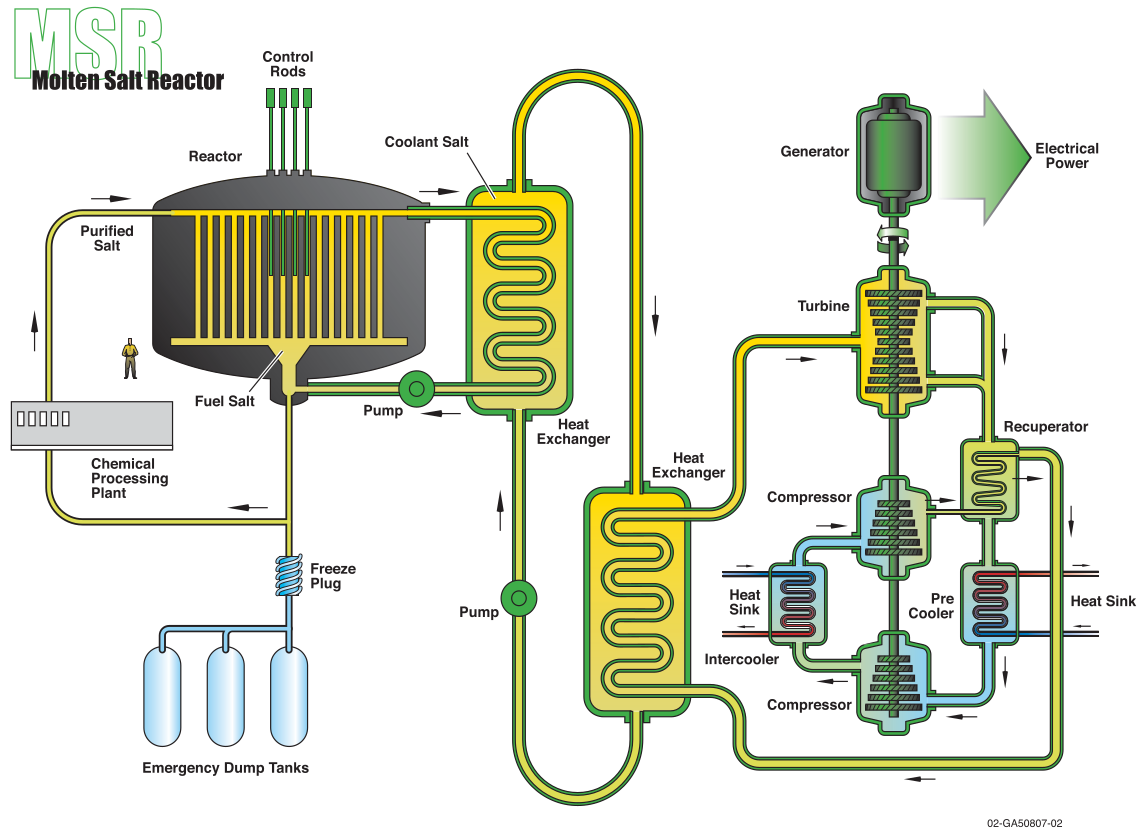
\includegraphics[width=.5\textwidth]{./images/msr}
      \caption{Schematic diagram of a general channel-type MSR concept
      \cite{u.s._doe_nuclear_energy_research_advisory_committee_technology_2002}.}
	  \label{fig:msr}
	\end{figure}
\end{frame}

\begin{frame}
  \frametitle{What is a Molten Salt Reactor (MSR)?}
  \textbf{Advantages of MSRs over other reactor types}
  \begin{itemize}
    \item Robust passive safety
      \begin{itemize}
        \item strong temperature feedback
        \item large thermal margin to boiling
      \end{itemize}
    \item Freeze plug drains fuel salt into containment tanks under emergency situations
    \item Online refueling and reprocessing can:
      \begin{itemize}
        \item reduce reactor downtime
        \item reduce required fissile inventory in reactor at any given time
        \item reduce transuranic waste produced
        \item allow for $^{233}$U breeding from $^{232}$Th
      \end{itemize}
    \item Viable as fast-spectrum breeder/burner reactor
    \item Can provide high-temperature heat for industrial heat applications
  \end{itemize}
\end{frame}

\begin{frame}
  \frametitle{Molten Salt Reactor Modeling \& Simulation}
  \textbf{While modeling MSRs is not necessarily more difficult than modeling solid-fueled
  reactors, we must adapt our software tools to accurately model phenomena unique to MSRs.}\\

  \textbf{Phenomena which pose challenges for MSR modeling}
  \begin{itemize}
	\item Strong multiphysics interactions involving neutron flux, temperature, and flow in the
      reactor core
	  \begin{itemize}
		\item Strong temperature feedback due to thermal expansion of liquid fuel salt
		\item Movement of \gls{DNP} along primary coolant loop
        \item Advection-dominated heat transfer
	  \end{itemize}
    \item Loss of delayed neutrons to out-of-core decay
    \item Complex turbulent flow effects in MSRs
  \end{itemize}
\end{frame}


\subsection{Moltres}
\section{Modeling Approach with Moltres} \label{sec:model}

This section describes the specific modeling approach for
simulating the CNRS Benchmark cases in Moltres.

For this work\footnote{The input files for
all benchmark
cases are available on the Moltres GitHub repository at 
\url{https://github.com/arfc/moltres/tree/devel/problems/2021-cnrs-benchmark}.
}, I ran the benchmark cases on a uniformly-spaced mesh
of 200$\times$200 elements. Thus, the dimensions of each mesh element are
0.01m$\times$0.01m. I adopted the group constant data
provided by Tiberga et al. \cite{tiberga_results_2020}. Next, I
discretized most variables, i.e., neutron fluxes, velocity
components, pressure, and temperature, using continuous, first-order, Lagrange
shape functions. The only exception is the precursor concentration variables,
which I discretized using zeroth-order monomial shape functions and solved
using a \gls{DFEM}. I interpolated the resulting discontinuous,
cell-centered precursor values to obtain the nodal values for results
analysis.

The
\texttt{Navier-Stokes} and \texttt{Heat} \texttt{Conduction} modules from
\gls{MOOSE} provide some of the capabilities for
modeling incompressible flow and heat transfer. In particular, I stabilized
the incompressible flow and temperature governing equations using the
\gls{SUPG} stabilization method implemented in \gls{MOOSE}
\cite{peterson_overview_2018}. Without \gls{SUPG} stabilization, I
observed spurious numerical oscillations in the velocity and temperature near
the top boundary due to the singularity on the top left corner where different
velocity boundary conditions meet. I also applied the \gls{PSPG} stabilization
scheme \cite{hughes_new_1986} from the Navier-Stokes module
\cite{peterson_overview_2018},
which enables equal-order discretizations in the velocity and pressure
variables. Equal-order discretizations with \gls{PSPG} are computationally
cheaper and more convenient than implementing higher-order
velocity discretizations for stability without \gls{PSPG}
\cite{chapelle_inf-sup_1993}.

Using the inverse power method solver in \gls{MOOSE}, I ran all eigenvalue calculations in
Steps 0.2, 1.1, 1.2, 1.3, and 1.4. I ran all other steps
using the Preconditioned Newton-Krylov solver
\cite{gaston_physics-based_2015}. The coupled steady-state problems in
Steps 1.2, 1.3, and 1.4 required segregated solvers for the neutronics
and the thermal-hydraulics due to the unique problem setups involving a
criticality search problem for the neutron multiplication factor
and a steady-state problem in thermal-hydraulics simultaneously.

\begin{table}[tb]
    \caption{Timestep sizes used for the time-dependent cases in
    Step 2.1, corresponding to 1/200th of the perturbation period.}
	\centering
	\setlength\tabcolsep{2.5pt}
	\begin{tabular}{l l l l l l l l}
	    \toprule
	    Frequency [Hz] & 0.0125 & 0.025 & 0.05 & 0.1 & 0.2 & 0.4 & 0.8 \\
	    \midrule
	    Timestep size [s] & 0.2 & 0.2 & 0.1 & 0.05 & 0.025 & 0.0125 & 0.00625
	    \\
	    \bottomrule
	\end{tabular}
	\label{table:timestep}
\end{table}

For the time-dependent cases in Step 2.1, I employed full coupling with
a second-order implicit Backward Differential Formula (BDF2) time-stepping
scheme. I set the timestep sizes for each driving frequency in the heat transfer
coefficient to 1/200th of the perturbation period. Table
\ref{table:timestep} shows the timestep sizes. I assumed the
systems reached asymptotic behavior when the magnitudes of neighboring power
peaks differed by less than 0.001\% for at least ten wavelengths. Under this
assumption, the phase shift measurements between adjacent waves always
converged before the magnitude measurements of the power peaks.

Table \ref{table:software} compares the numerical methods, meshing schemes, and
neutronics models of Moltres and the four participating software packages in
the CNRS benchmark paper \cite{tiberga_results_2020}. The $SP_N$ and
$S_N$ neutronics models refer to the simplified $P_N$ spherical harmonics and
$S_N$ discrete ordinates neutron transport models, respectively. Based on the
solvers and methods of solution, Moltres is most similar to the
PHANTOM-$S_N$ + DGFlows \cite{tiberga_discontinuous_2019} multiphysics package
from \gls{TUD} with the $S_2$ neutron transport model. Participants from
\gls{CNRS} and \gls{PSI}
employed non-uniform meshes which were refined near the boundaries. In contrast,
we and the \gls{PoliMi} and \gls{TUD} participants employed uniform meshes.

\FloatBarrier

\begin{landscape}
\begin{table*}[p]
    \caption{List of software packages and their corresponding model
    specifications for the CNRS Benchmark simulations
    \cite{tiberga_results_2020}.}
    \centering
    \begin{tabular}{p{4.2cm} p{7cm} p{3.3cm} p{2cm} p{2.7cm}}
        \toprule
        Software & Institute & Numerical method & Mesh & Neutronics model \\
        \midrule
        OpenFOAM & Centre national de la recherche scientifique (CNRS) & Finite volume & 200$\times$200 \newline Non-uniform & $SP_1$ \& $SP_3$ \\
        OpenFOAM & Politecnico di Milano (PoliMi) & Finite volume & 400$\times$400 \newline Uniform & Neutron diffusion \\
        GeN-Foam & Paul Scherrer Institute (PSI) & Finite volume & 200$\times$200 \newline Non-uniform & Neutron diffusion \\
        PHANTOM-$S_N$+DGFlows & Delft University of Technology (TUD) & Discontinuous finite \newline element & 50$\times$50 \newline Uniform & $S_2$ \& $S_6$ \\
        Moltres (This work) & University of Illinois at Urbana-Champaign (UIUC) & Continuous \& discontinuous finite element & 200$\times$200 \newline Uniform & Neutron diffusion \\
        \bottomrule
    \end{tabular}
    \label{table:software}
\end{table*}
\end{landscape}

\FloatBarrier

\subsection{Objectives}
\begin{frame}
  \frametitle{Objectives}
  \begin{block}{\textbf{Objectives}}
    \begin{enumerate}
      \item \textbf{Verify and Validate Existing Multiphysics Coupling Capabilities in Moltres}
      \item \textbf{Implement a RANS-based Turbulence Model in Moltres}
      \item \textbf{Develop a Hybrid Neutronics Method for Control Rod Modeling}
    \end{enumerate}
  \end{block}
\end{frame}


\section{Objective 1: Verification \& Validation}
\subsection{Motivation for MSR Multiphysics Modeling V\&V}
\begin{frame}
  \frametitle{MSR Multiphysics Modeling V\&V}
  \begin{columns}
    \column{5.5cm}
      \textbf{Three important multiphysics phenomena in MSRs}
      \begin{itemize}
        \item Salt flow-induced temperature and delayed neutron precursor (DNP) drift
        \item Temperature reactivity feedback due to Doppler broadening and thermal expansion
        \item Buoyancy-driven flow due to temperature gradients
      \end{itemize}
    \column{5.5cm}
      \begin{figure}
        \centering
        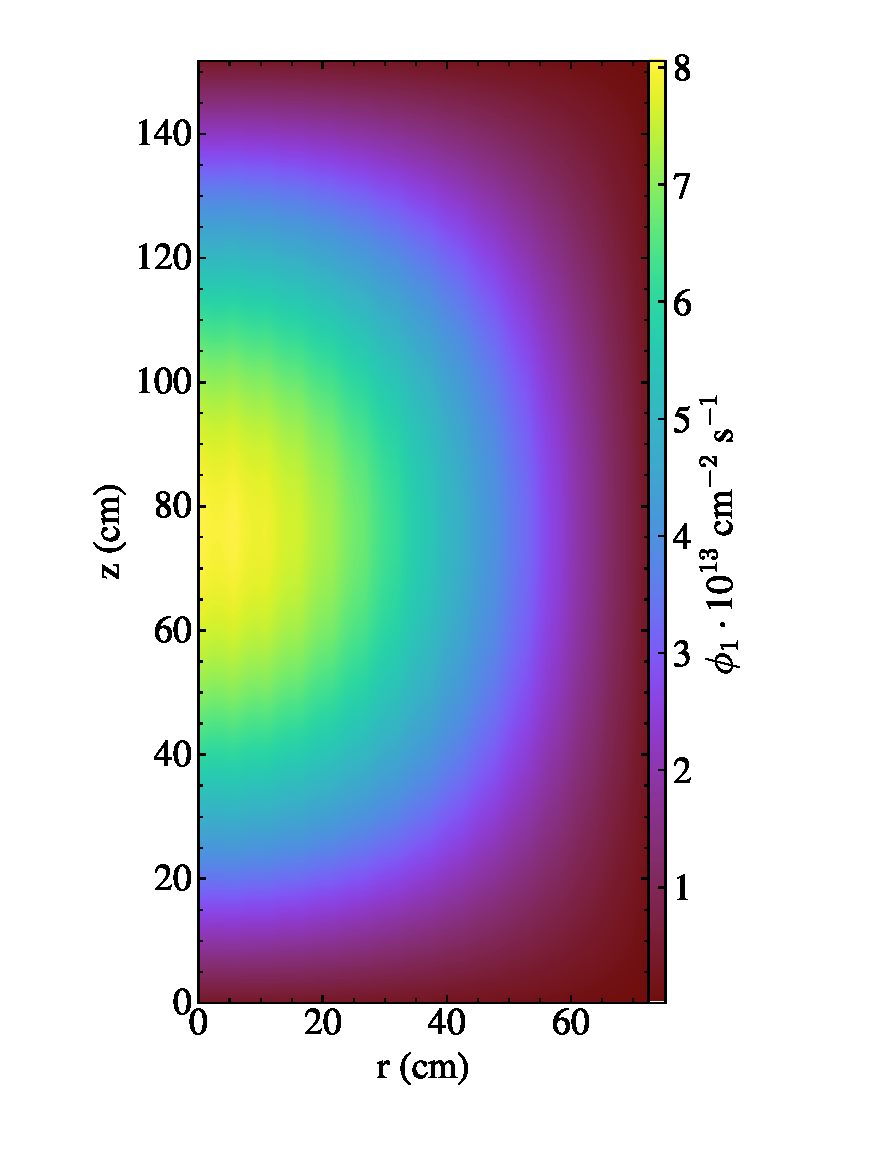
\includegraphics[width=.48\columnwidth]{../images/2d_gamma_heating_group1}
        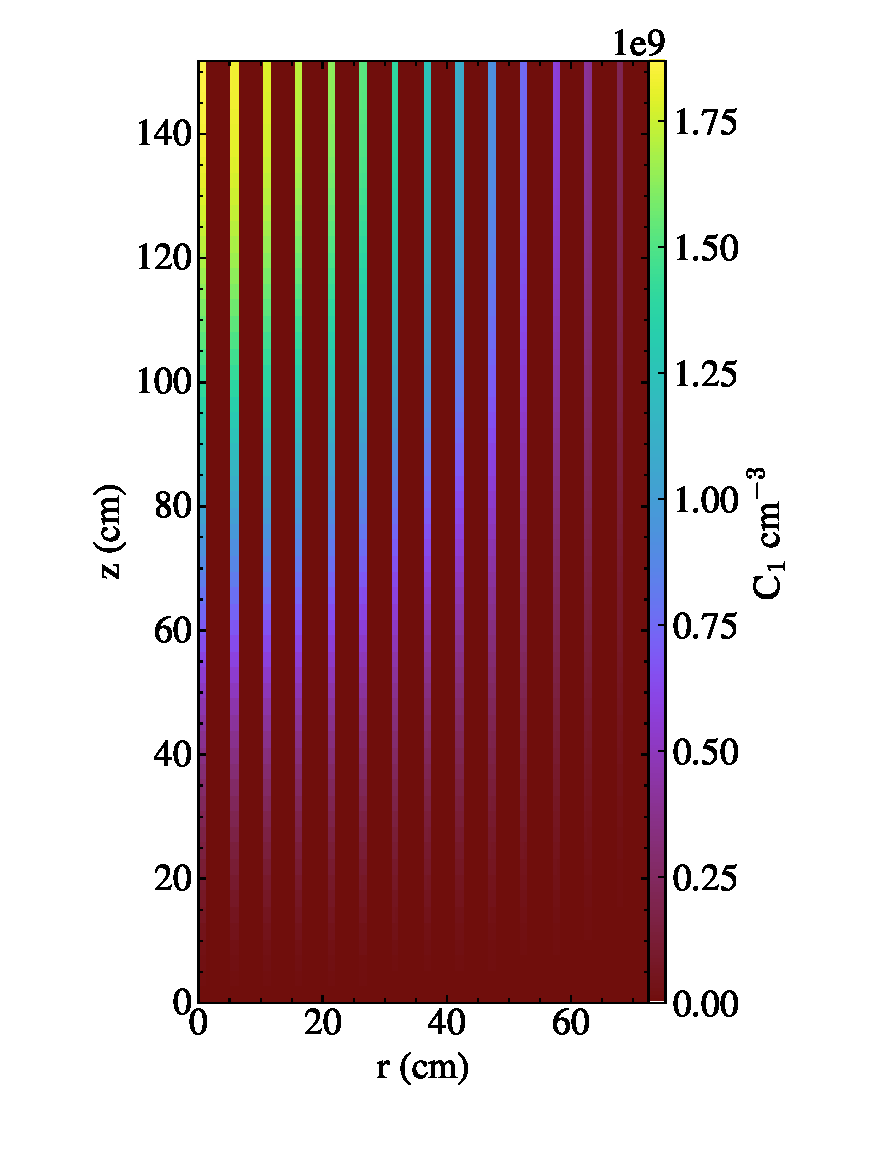
\includegraphics[width=.48\columnwidth]{images/2d_gamma_heating_pre1_scaled}
        \caption{Group 1 neutron flux (left) and the longest-lived precursor group (right) in a 2-D
        MSRE model with upward flow \cite{lindsay_introduction_2018}.}
      \end{figure}
  \end{columns}
\end{frame}

\subsection{Study 1: Verification of Moltres with the CNRS Benchmark}
\begin{frame}
  \frametitle{V\&V Study 1: Verification of Moltres with the CNRS Benchmark}

  Published in \textit{Verification of Moltres for Multiphysics Simulations of Fast-Spectrum Molten
    Salt Reactors, Annals of Nuclear Energy, Volume 173, 2022.}

  \begin{columns}
    \column[t]{6.5cm}
    \begin{block}{\textbf{CNRS Benchmark \cite{tiberga_results_2020}}}
      \begin{itemize}
        \item A numerical benchmark for multiphysics software dedicated to modeling ``pool-type''
          fast-spectrum MSRs
        \item Problem Setup
          \begin{itemize}
            \item 2-D, 2m-by-2m cavity
            \item LiF-BeF$_2$-UF$_4$ molten salt
            \item Six neutron energy groups
            \item Eight precursor groups
            \item Volumetric conjugate heat sink term
            \item Incompressible flow
          \end{itemize}
      \end{itemize}
    \end{block}
    \column[t]{3.5cm}
    \begin{figure}
      \centering
      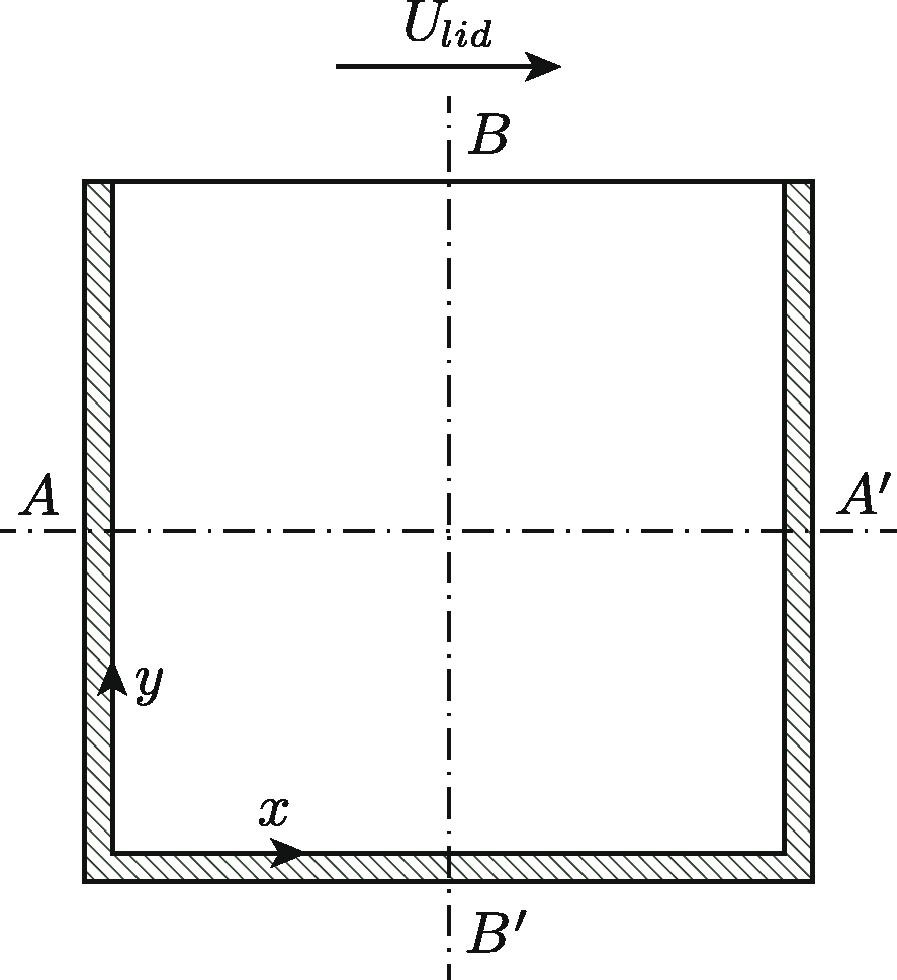
\includegraphics[width=\columnwidth]{../images/cnrs-geometry}
      \caption{CNRS benchmark problem domain \cite{tiberga_results_2020}}
    \end{figure}
  \end{columns}
\end{frame}

\begin{frame}
  \frametitle{V\&V Study 1: Verification of Moltres with the CNRS Benchmark}

  Published in \textit{Verification of Moltres for Multiphysics Simulations of Fast-Spectrum Molten
    Salt Reactors, Annals of Nuclear Energy, Volume 173, 2022.}

  \begin{columns}
    \column[t]{6.5cm}
    \begin{block}{\textbf{CNRS Benchmark \cite{tiberga_results_2020}}}
      \begin{itemize}
        \item Consists of three phases
          \begin{itemize}
            \item Phase 0: Single-physics verification
              \begin{itemize}
                \item Step 0.1: Velocity field
                \item Step 0.2: Neutronics
                \item Step 0.3: Temperature
              \end{itemize}
            \item Phase 1: Steady-state coupling
              \begin{itemize}
                \item Step 1.1: Circulating fuel
                \item Step 1.2: Power coupling
                \item Step 1.3: Buoyancy
                \item Step 1.4: Full coupling
              \end{itemize}
            \item Phase 2: Time-dependent coupling
              \begin{itemize}
                \item Step 2.1: Forced convection transient
              \end{itemize}
          \end{itemize}
      \end{itemize}
    \end{block}
    \column[t]{3.5cm}
    \begin{figure}
      \centering
      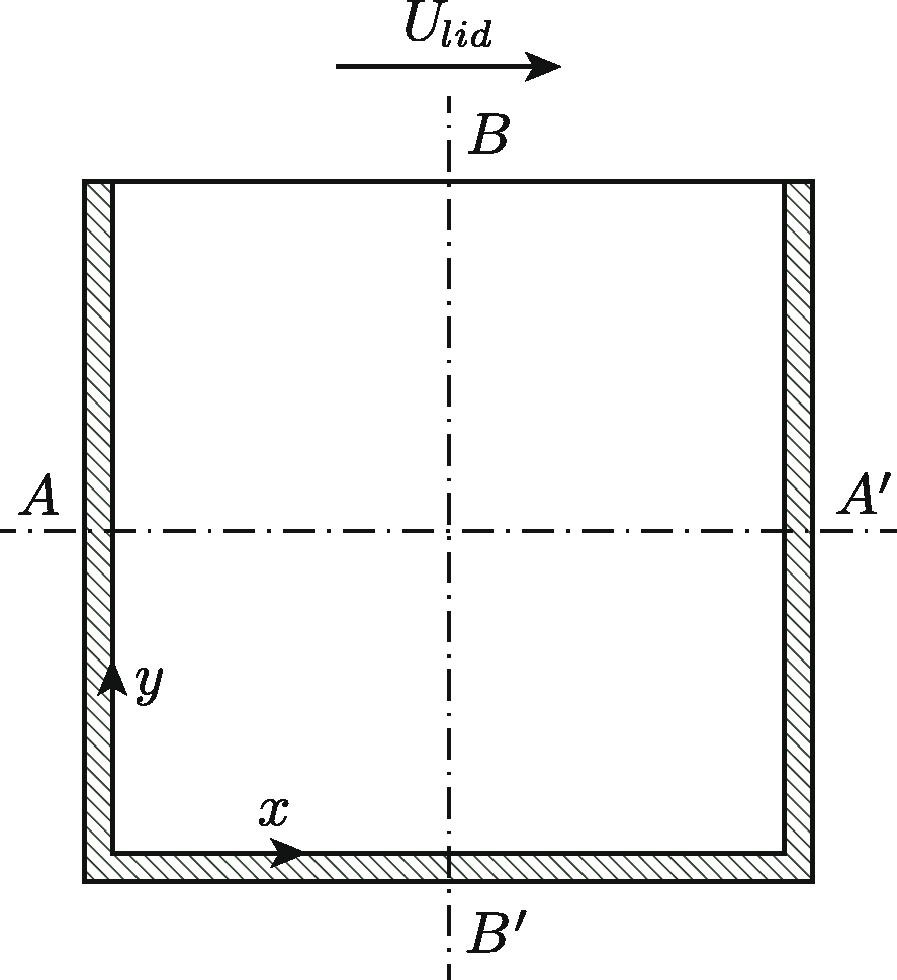
\includegraphics[width=\columnwidth]{../images/cnrs-geometry}
      \caption{CNRS benchmark problem domain \cite{tiberga_results_2020}}
    \end{figure}
  \end{columns}
\end{frame}

\begin{frame}
  \frametitle{V\&V Study 1: Verification of Moltres with the CNRS Benchmark}
  \textbf{Outcome: Moltres is consistent with the other multiphysics software in the benchmark
  problems.}
  \begin{columns}
    \hfill
    \column[t]{4cm}
    \vspace{.3cm}
    \begin{figure}
      \centering
      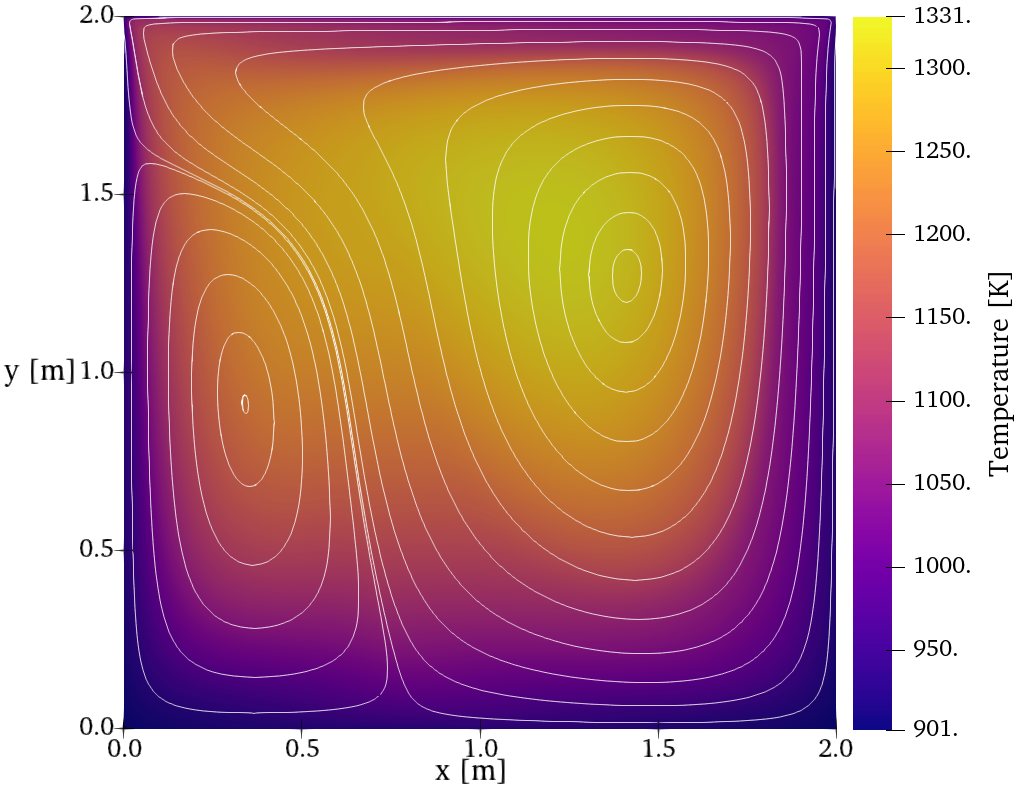
\includegraphics[width=\columnwidth]{../images/full-coupled}
      \caption{Step 1.4 - Temperature distribution and flow streamlines for the fully
        coupled system.}
    \end{figure}
    \column[t]{4cm}
    \begin{figure}
      \centering
      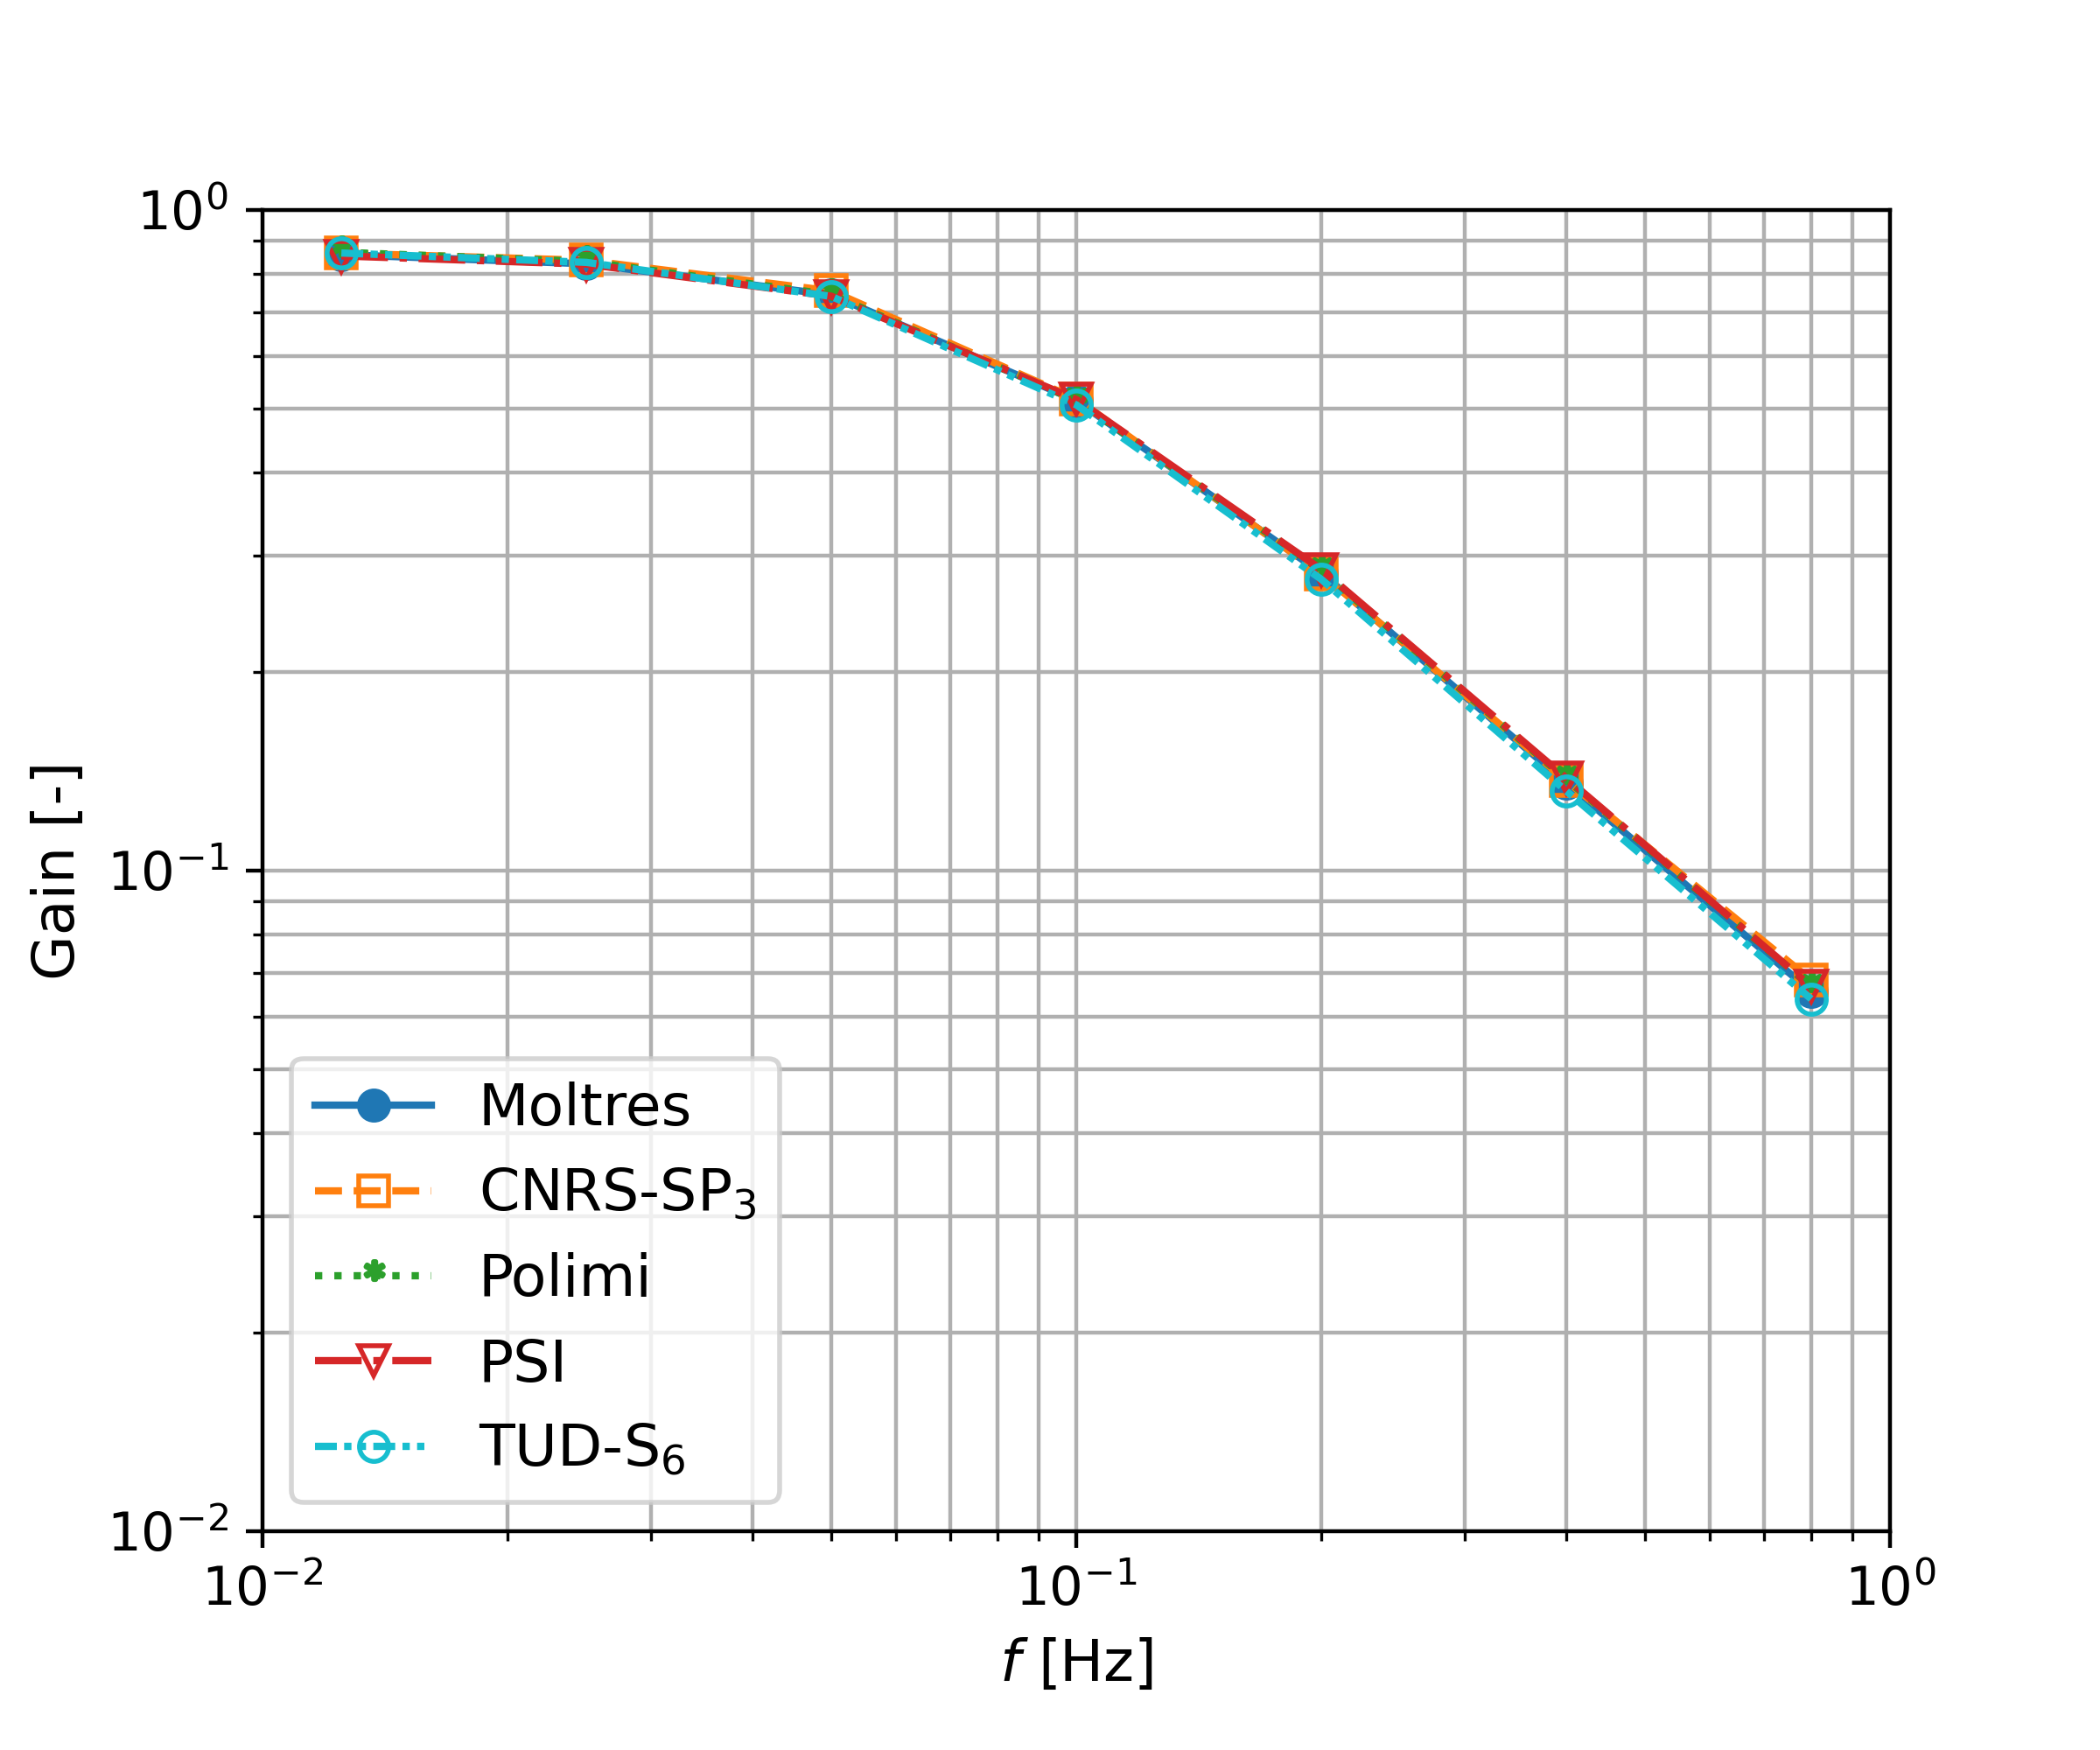
\includegraphics[width=\columnwidth]{../images/2-1-gain-plot}
      \caption{Step 2.1 - Bode gain plot of the frequency response of the fully
      coupled system.}
    \end{figure}
    \column[t]{4cm}
    \begin{figure}
      \centering
      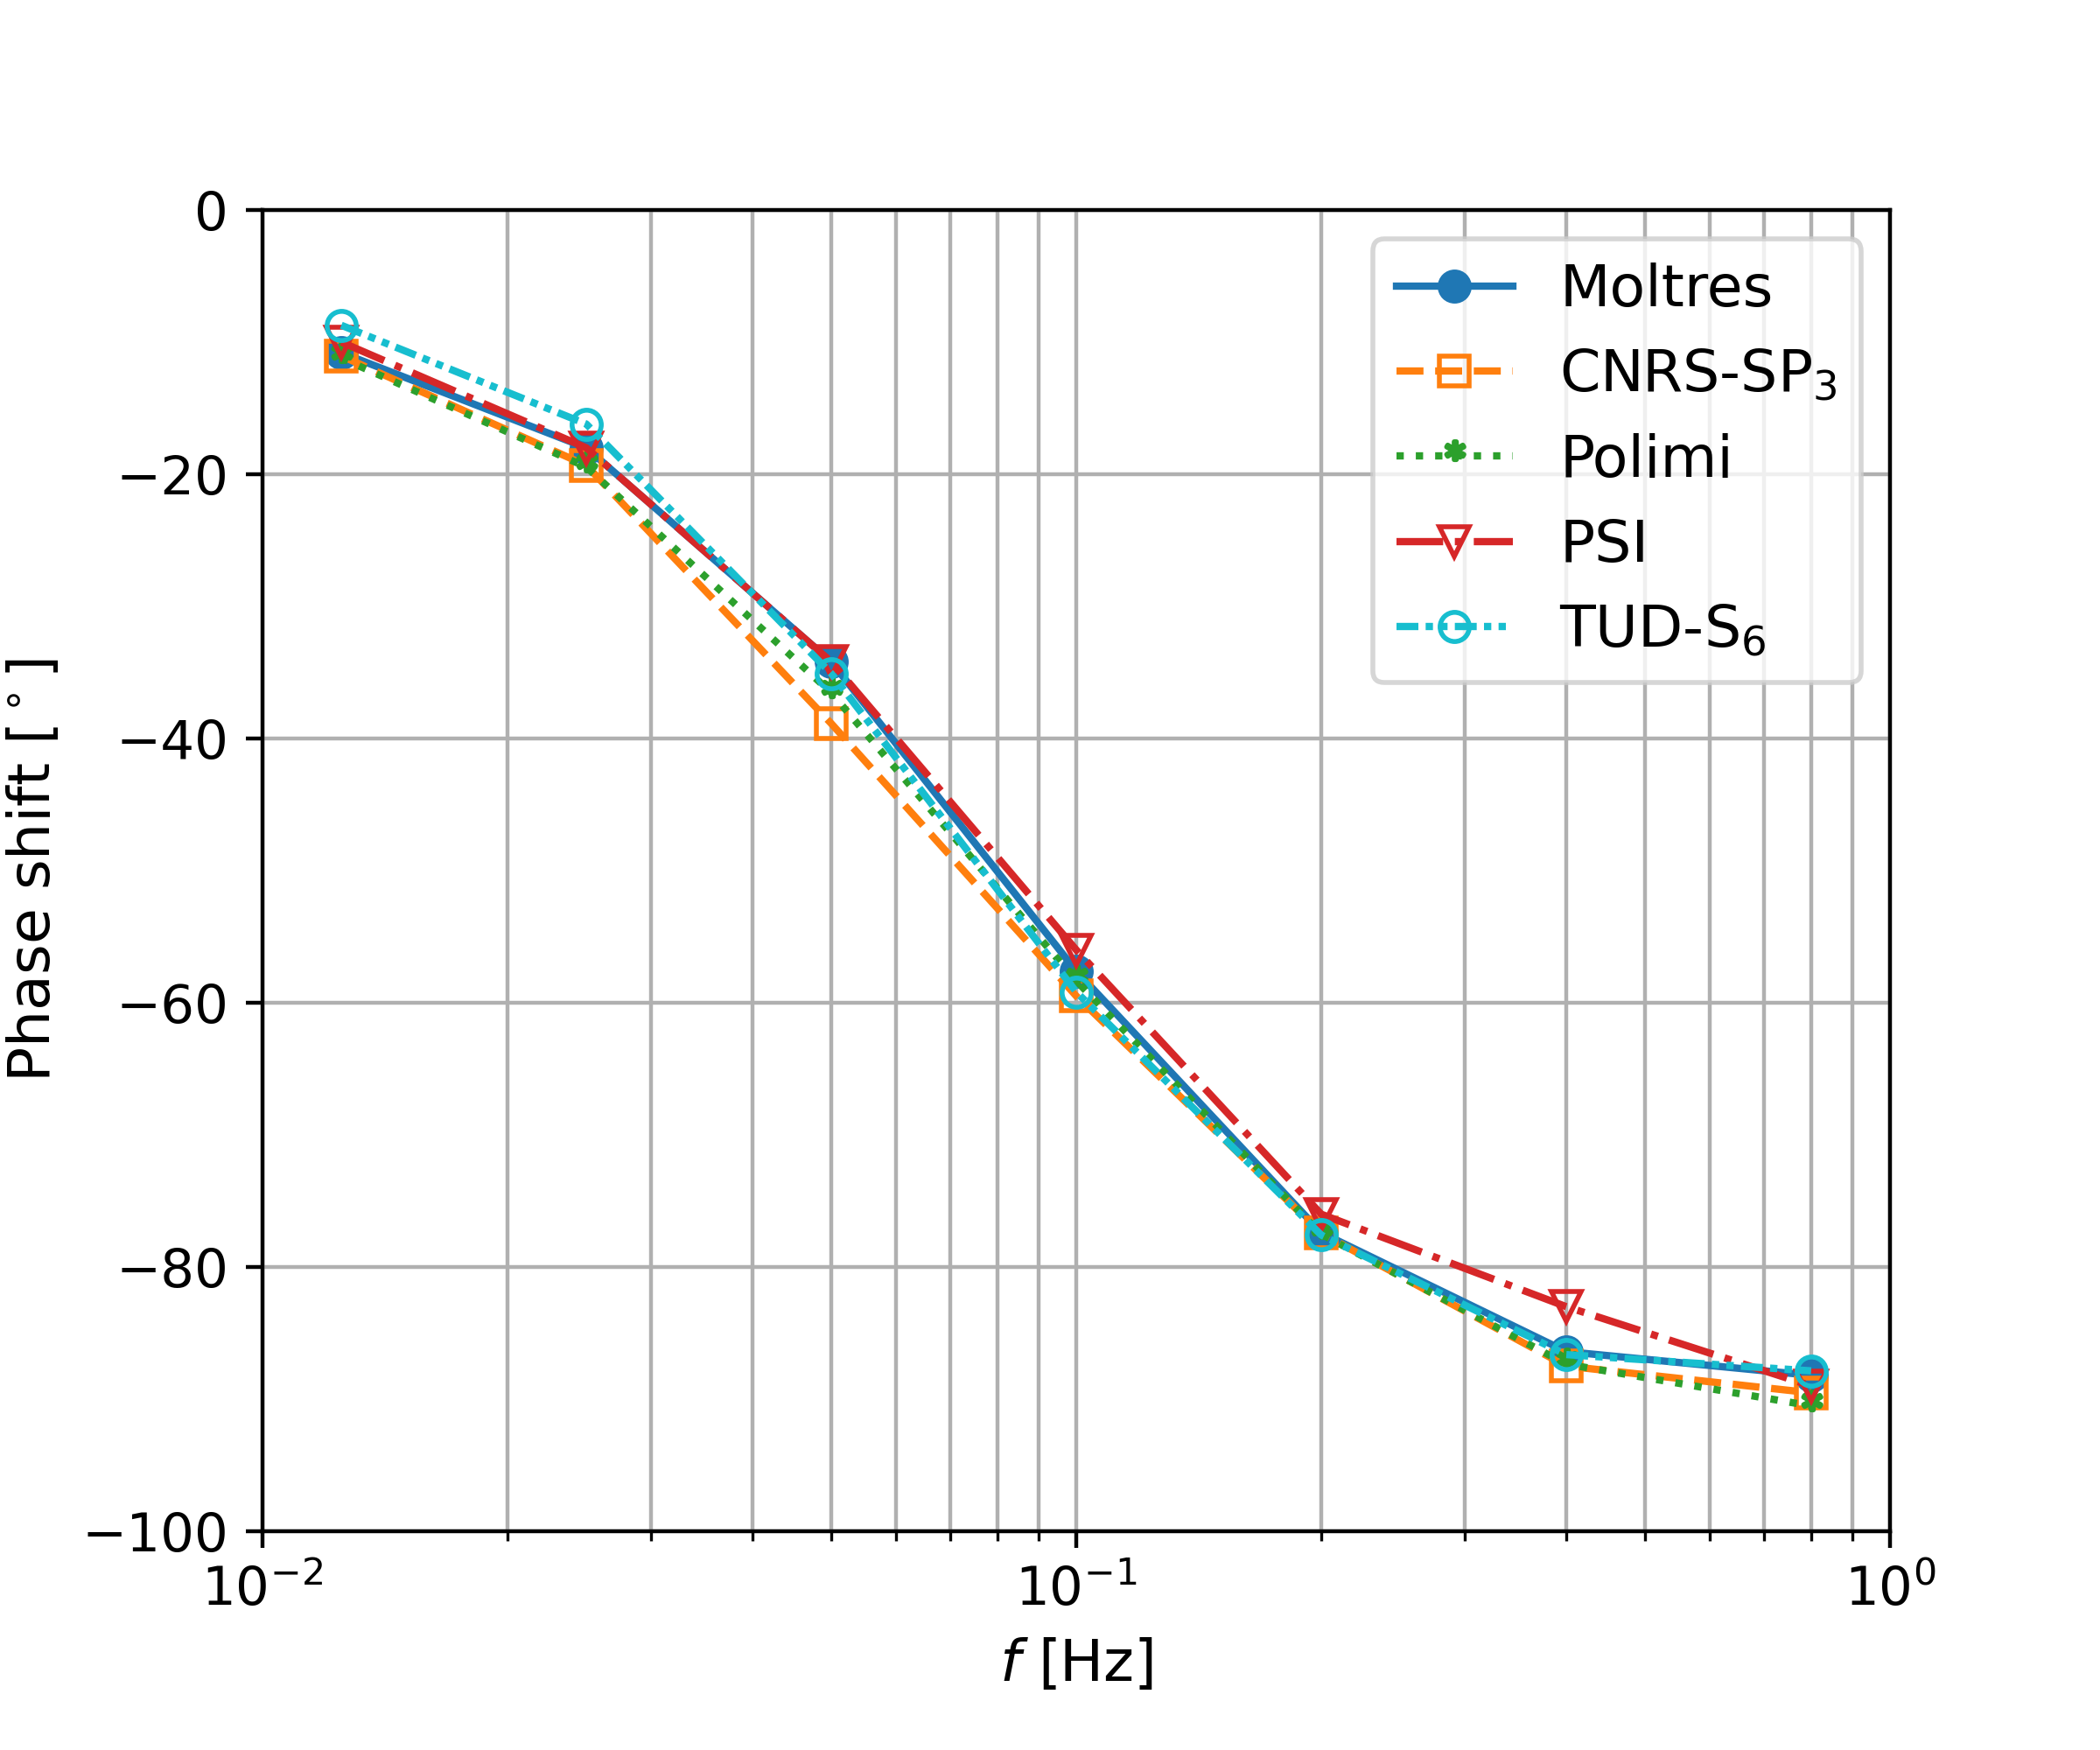
\includegraphics[width=\columnwidth]{../images/2-1-phase-plot}
      \caption{Step 2.1 - Bode phase plot of the frequency response of the fully
      coupled system.}
    \end{figure}
    \hfill
  \end{columns}
\end{frame}

\subsection{Study 2: MSRE Pump Start-up \& Coast-Down Transients}
\begin{frame}
  \frametitle{V\&V Study 2: MSRE Pump Start-up \& Coast-Down Transients}
  This study is based on two transient flow-rate tests on the MSRE under zero-power conditions.
  Starting from zero power critical states with/without forced flow, the fuel salt pump was coasted
  down/started up.
  \begin{columns}
    \column[t]{5.5cm}
    \begin{figure}
      \centering
      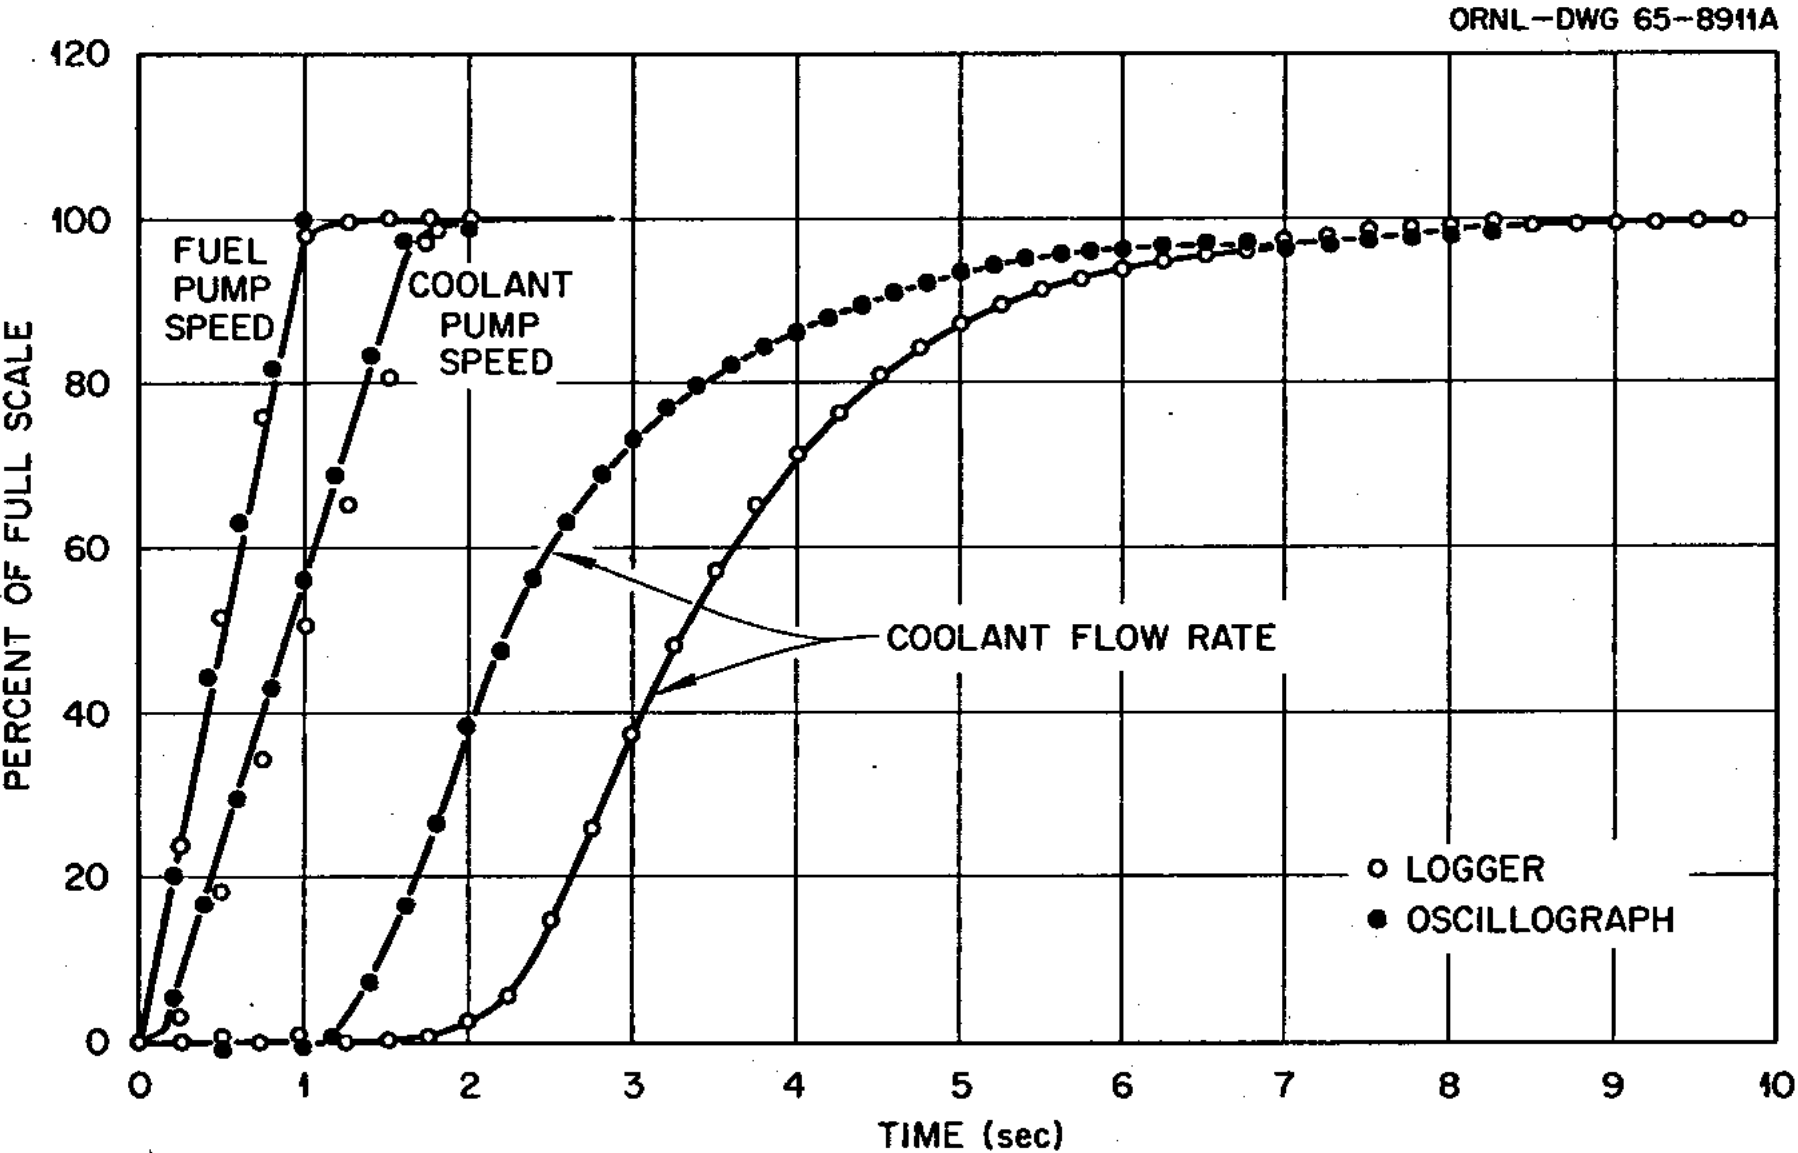
\includegraphics[width=.8\columnwidth]{images/msre-startup}
      \caption{Start-up pump speed and flow rate \cite{prince_zero-power_1968}.}
    \end{figure}
    \column[t]{5.5cm}
    \begin{figure}
      \centering
      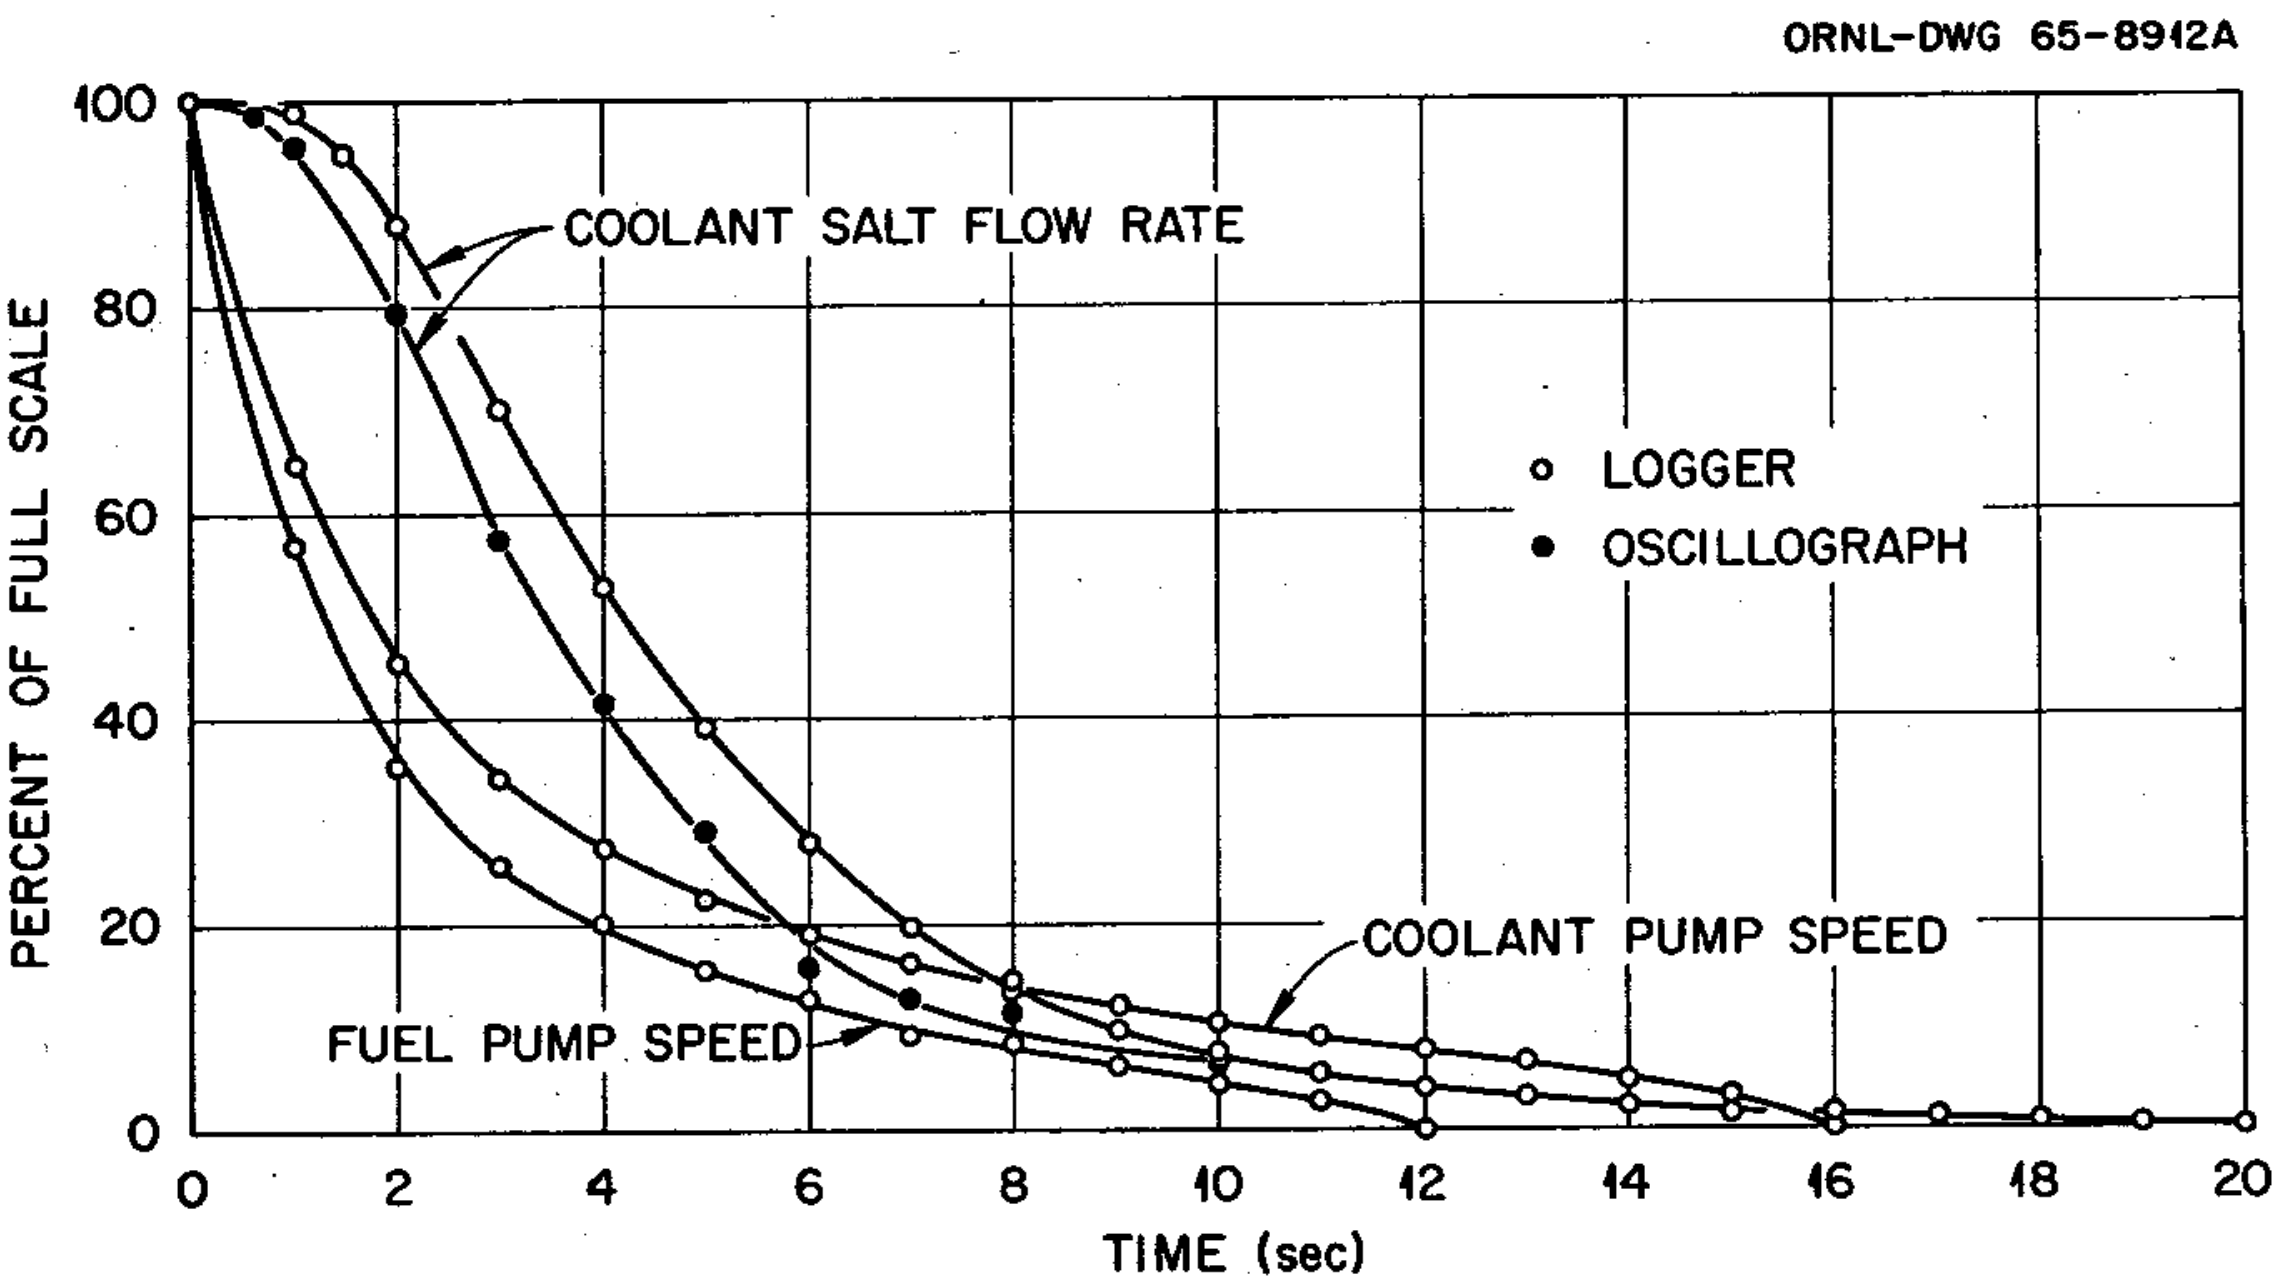
\includegraphics[width=.95\columnwidth]{images/msre-coastdown}
      \caption{Coast-down pump speed and flow rate \cite{prince_zero-power_1968}.}
    \end{figure}
  \end{columns}
\end{frame}

\begin{frame}
  \frametitle{V\&V Study 2: MSRE Pump Start-up \& Coast-Down Transients}
  \begin{columns}
    \column[t]{4cm}
    \begin{figure}
      \centering
      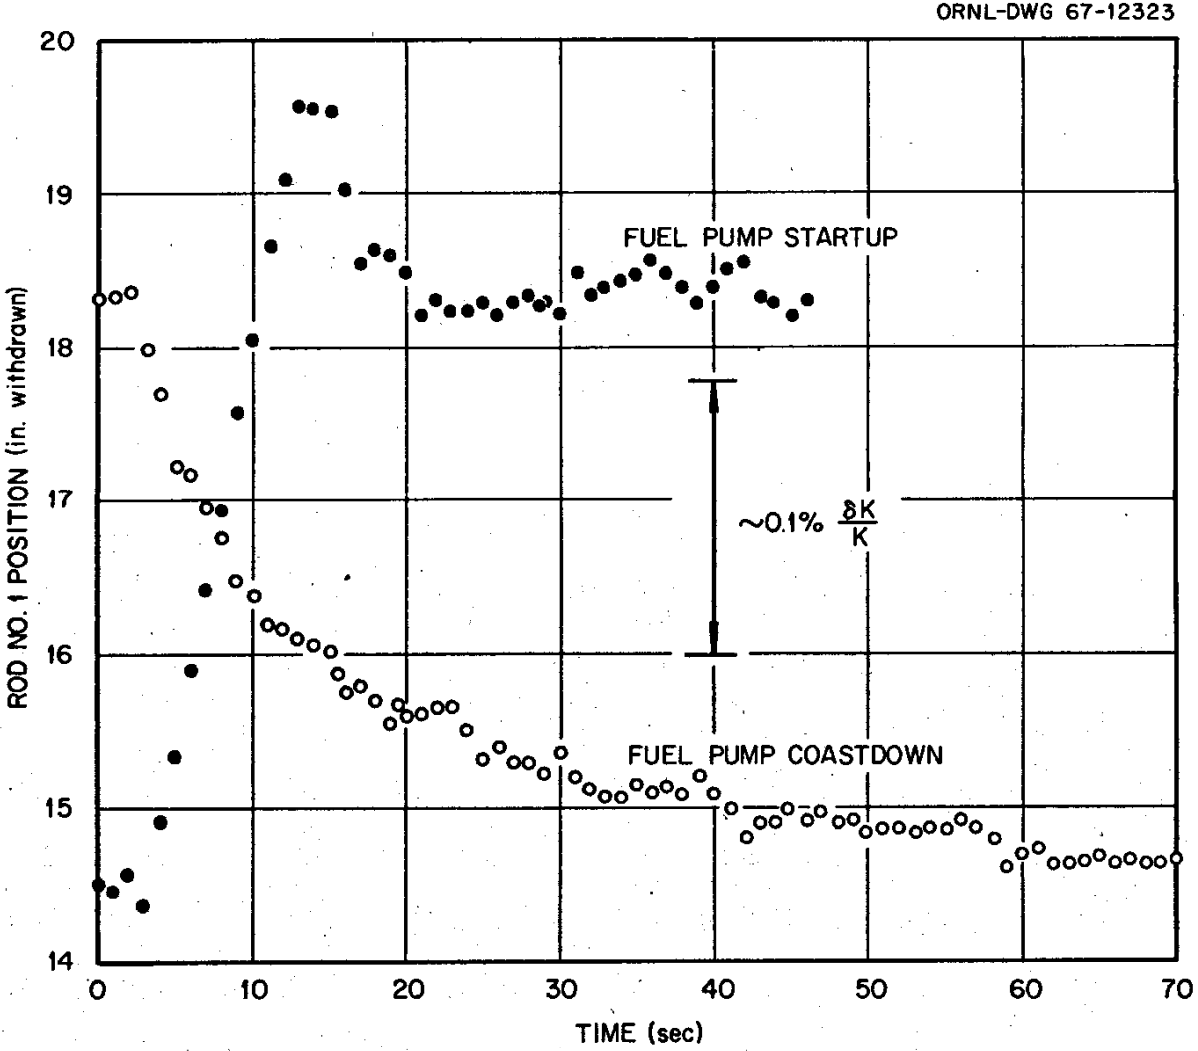
\includegraphics[width=.9\columnwidth]{../images/msre-transient}
      \caption{Control rod response to fuel pump start-up and coast-down
      \cite{prince_zero-power_1968}.}
    \end{figure}
    \hfill
    \column[t]{4cm}
    \begin{figure}
      \centering
      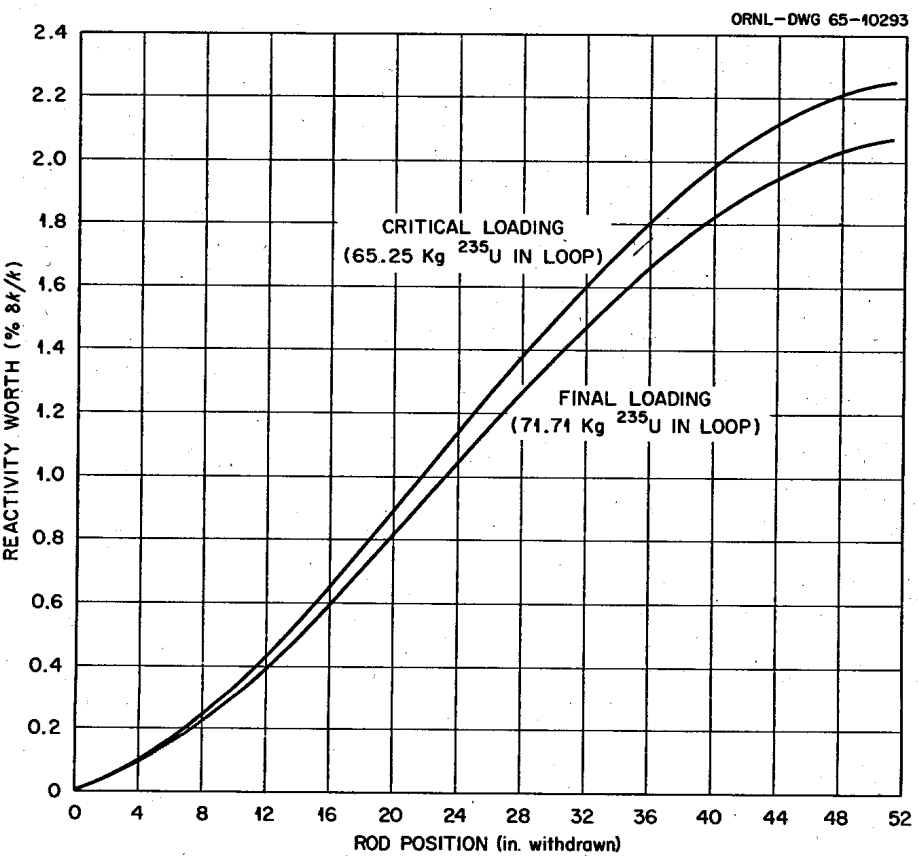
\includegraphics[width=.9\columnwidth]{../images/msre-rod-worth}
      \caption{Integral rod worth \cite{prince_zero-power_1968}.}
    \end{figure}
    \hfill
    \column[t]{4cm}
    \begin{figure}
      \centering
      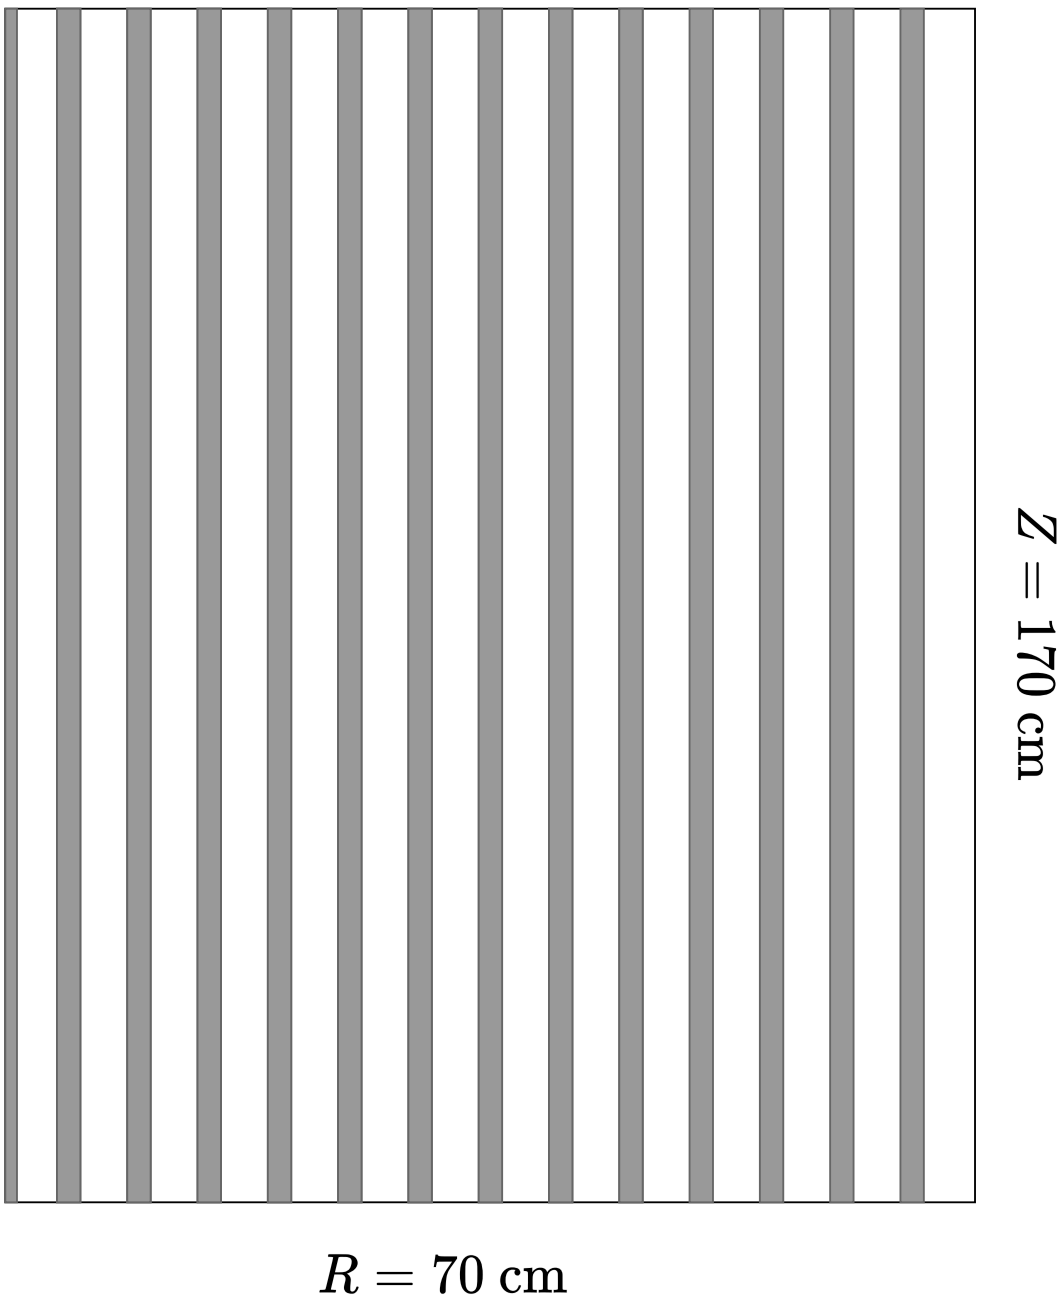
\includegraphics[width=.9\columnwidth]{images/msre-2d}
      \caption{2-D axisymmetric model of the MSRE.}
    \end{figure}
  \end{columns}
\end{frame}

\begin{frame}
  \frametitle{V\&V Study 2: MSRE Pump Start-up \& Coast-Down Transients}
  \begin{block}{\textbf{MSR Phenomena Involved}}
    \begin{itemize}
      \item DNP drift under time-varying flow
      \item Loss of delayed neutrons due to out-of-core DNP decay
    \end{itemize}
  \end{block}
  \begin{block}{\textbf{Aim of the study}}
    Reproduce the reactivity curve of the control rod response with a 2-D axisymmetric model of the
    MSRE in Moltres
  \end{block}
  \begin{block}{\textbf{Objectives}}
    \begin{itemize}
      \item Develop a verification benchmark based on the MSRE pump start-up \& coast-down
        transients that is easily reproducible
      \item Verify Moltres against QuasiMolto in collaboration with Aaron Reynolds
        (formerly at Oregon State University)
      \item Validate Moltres against MSRE experimental data for zero-power pump transients
    \end{itemize}
  \end{block}
\end{frame}

\begin{frame}
  \frametitle{V\&V Study 2: MSRE Pump Start-up \& Coast-Down Transients}
  \begin{columns}
    \column[t]{6.5cm}
    \begin{block}{\textbf{Current Status}}
      \begin{itemize}
        \item Moltres and QuasiMolto simulations (Complete)
        \item Data analysis is in progress (In progress)
        \item Submission for publication (In progress)
      \end{itemize}
    \end{block}
    \begin{block}{\textbf{Extension}}
      Add the upper and lower plena in the 2-D axisymmetric model for improved validation with
      the MSRE experimental data.

      Plena modeling options:
      \begin{enumerate}
        \item Rectangular block with perfect mixing and 1-D flow
        \item Dome-shaped domains with turbulent flow modeling
      \end{enumerate}
    \end{block}
    \column[t]{4.5cm}
    \begin{figure}
      \centering
      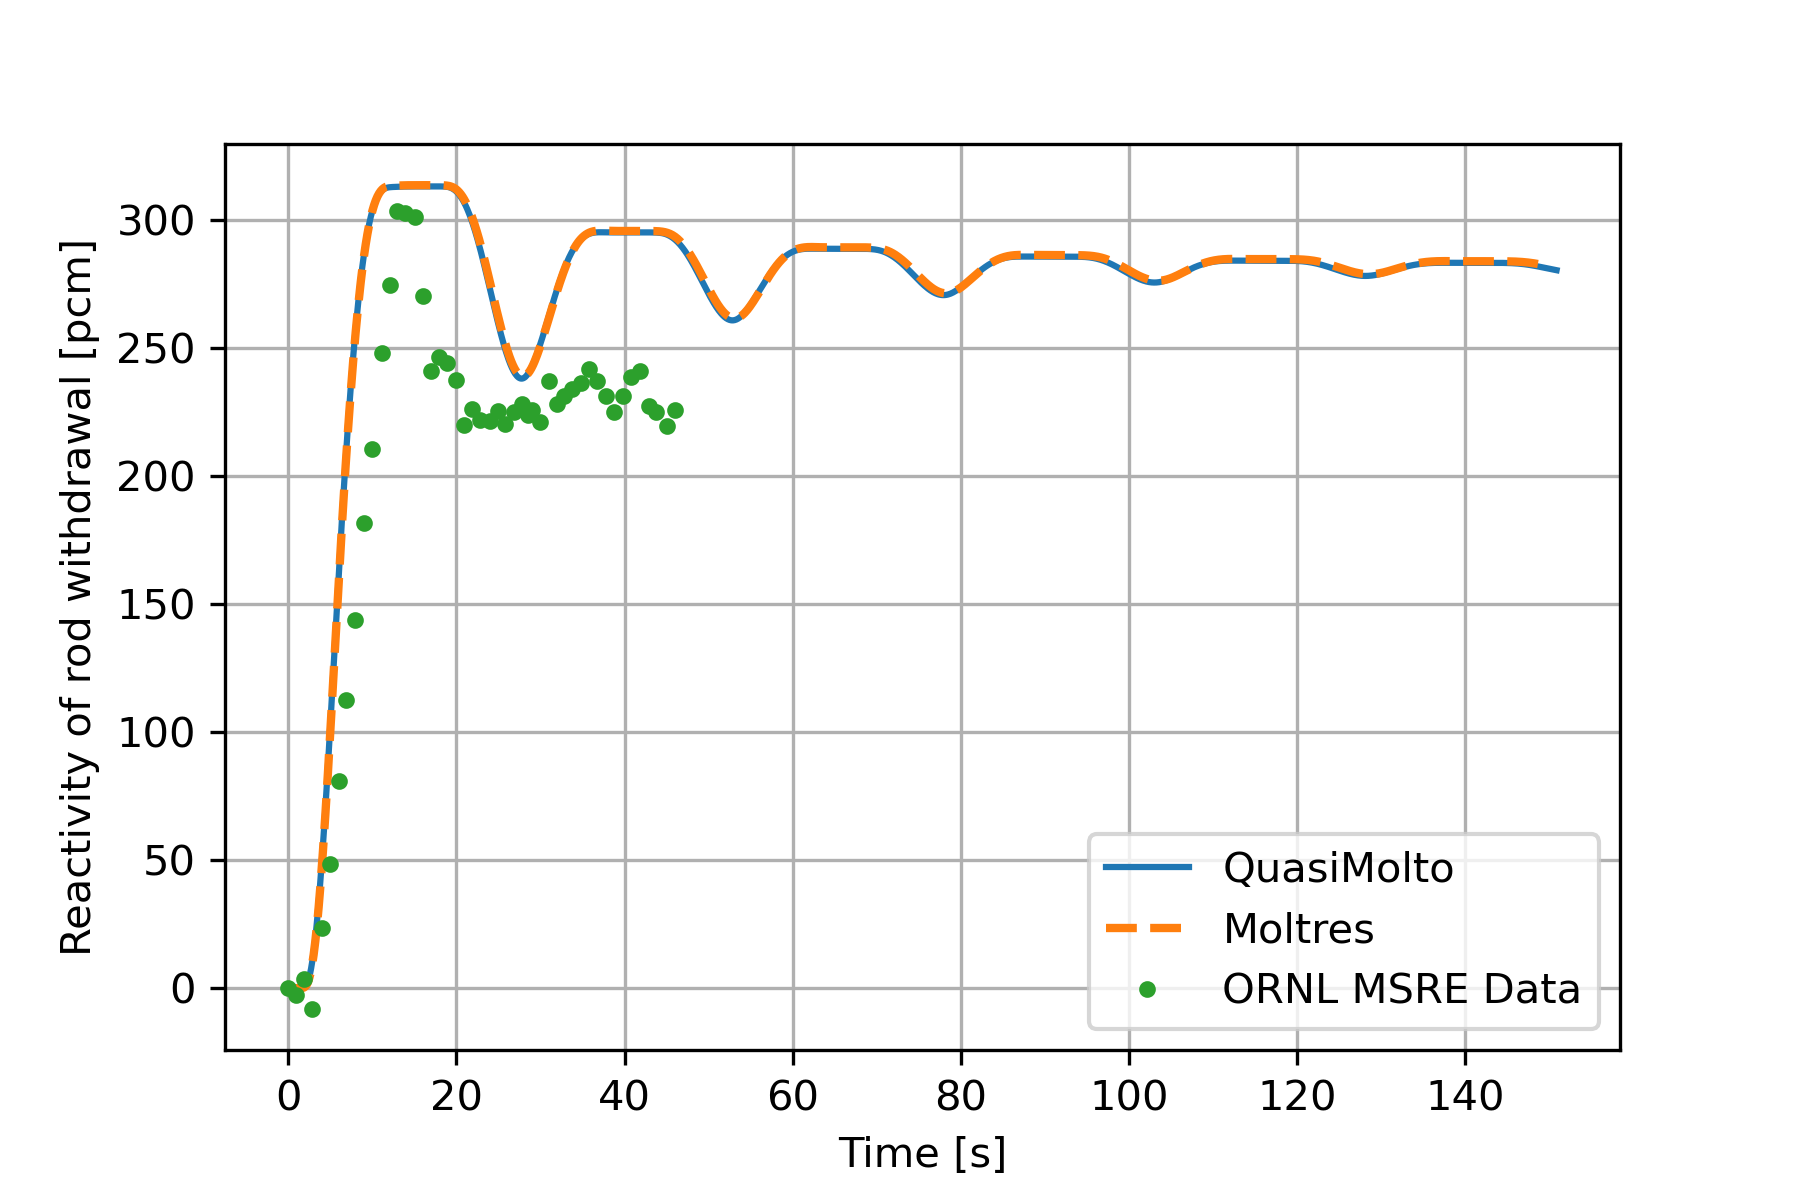
\includegraphics[width=.9\columnwidth]{images/start-up-v2-reactivity}
      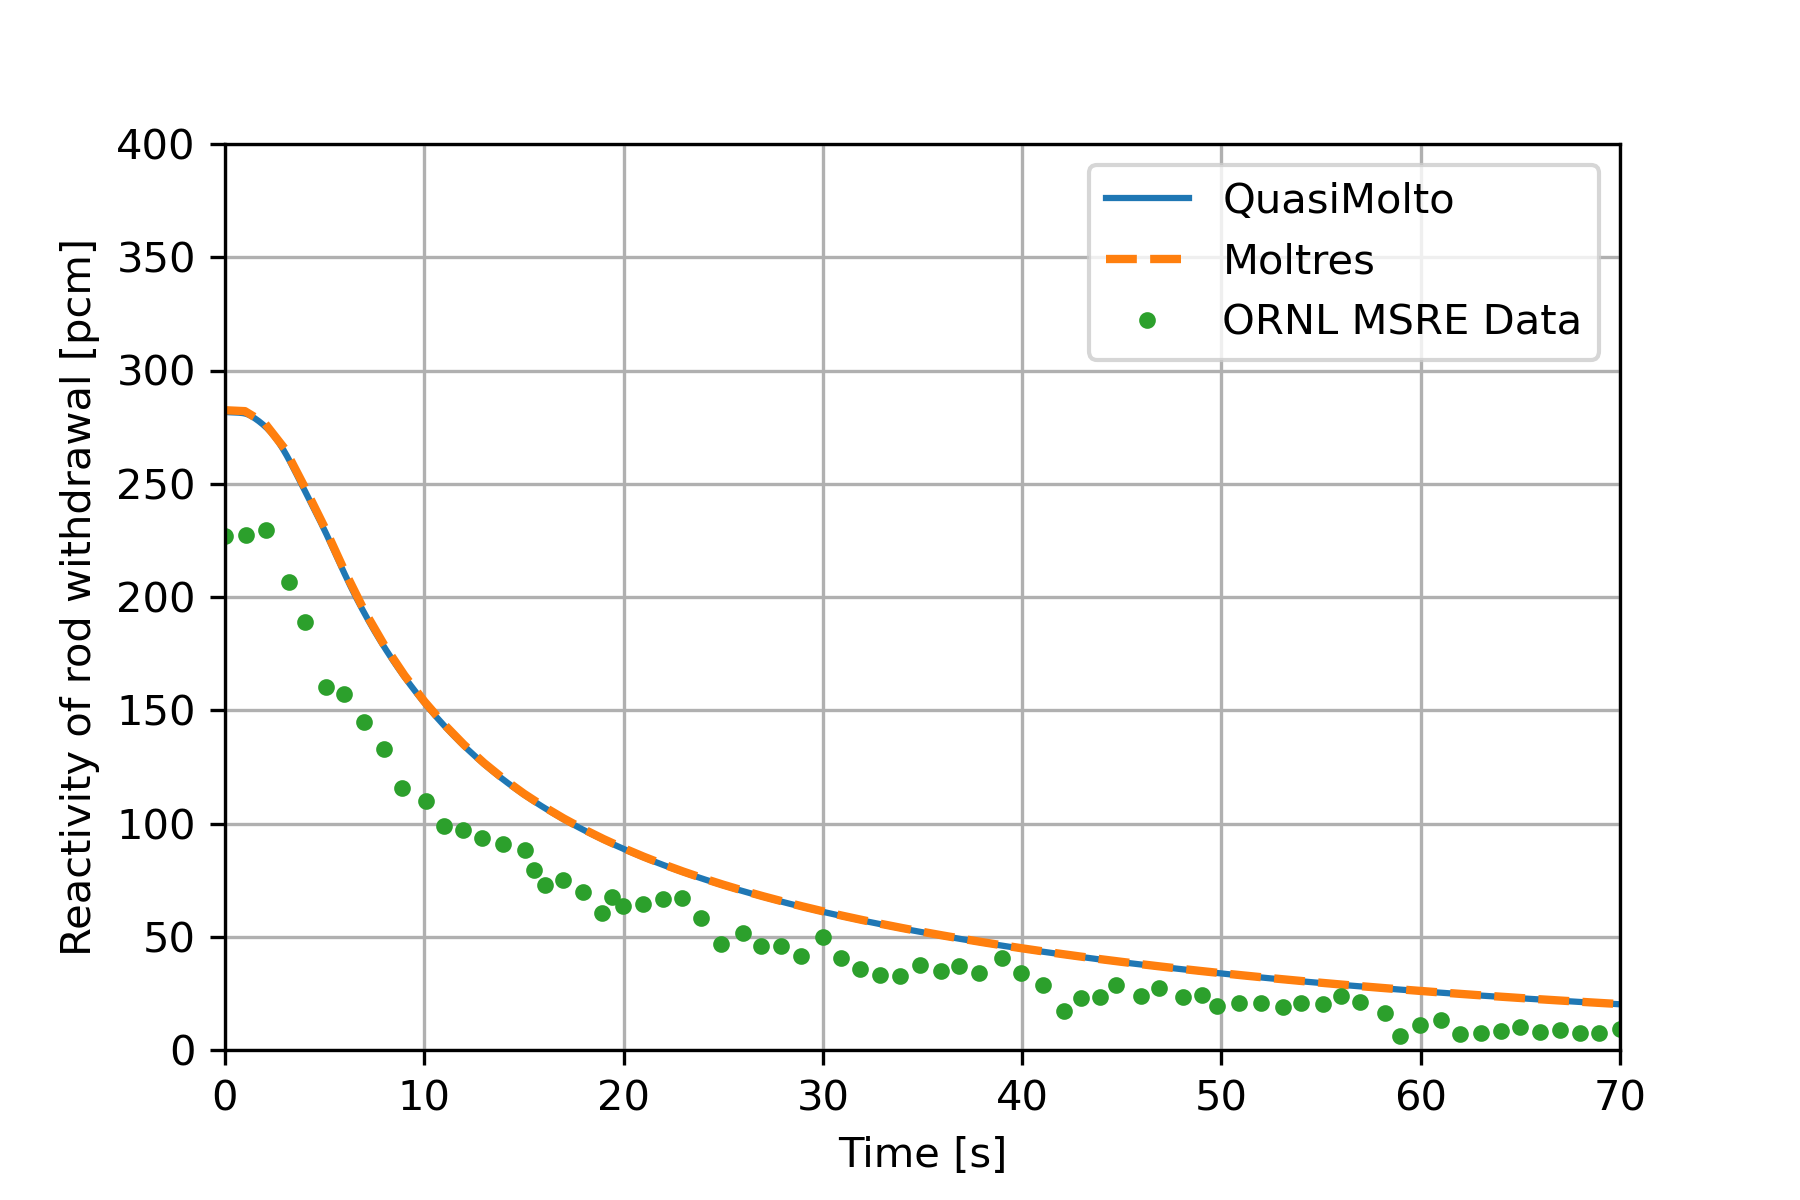
\includegraphics[width=.9\columnwidth]{images/coast-down-v2-reactivity}
      \caption{Reactivity change during the pump start-up (top) and coast-down (bottom)
      transients.}
    \end{figure}
  \end{columns}
\end{frame}



\section{Objective 2: Turbulence Modeling}
\subsection{Motivation for Turbulence Modeling Implementation}
\begin{frame}
  \frametitle{Motivation for Turbulence Modeling Implementation}
  \textbf{Turbulent Flows in MSRs}
  \begin{itemize}
    \item The Reynolds number of salt flow in MSRs can range from $10^3$ in MSRE fuel channels
      \cite{kedl_fluid_1970} to $10^6$ in the MSFR core \cite{fiorina_modelling_2014}
    \item Turbulent effects expected in MSRs
    \begin{itemize}
      \item Turbulent diffusion of heat and \gls{DNP}
      \item Flow separation and recirculation zones due to abrupt geometry changes
    \end{itemize}
    \item Temperature hotspots may induce thermal stress on structural
      components and temperature-induced reactivity effects
  \end{itemize}
  \pause
  \begin{block}{\textbf{Area of Improvement for Moltres for MSR Modeling}}
    \begin{itemize}
      \item Moltres does not currently have turbulence modeling capability for simulating
        turbulent flows in MSRs
    \end{itemize}
  \end{block}
\end{frame}

\subsection{Turbulence Models}
\begin{frame}
  \frametitle{Turbulence Models}
  Numerous types of turbulence models exist of various turbulent flow applications. By order of
  increasing computational complexity:
  \begin{itemize}
      \item RANS-based models
      \begin{itemize}
          \item Eddy viscosity models
          \begin{itemize}
              \item Algebraic models
              \item One- and two-equation models
          \end{itemize}
          \item \gls{RSM}
      \end{itemize}
      \item \gls{DES}
      \item \gls{LES}
      \item \gls{DNS}
  \end{itemize}
\end{frame}

\begin{frame}
  \frametitle{Turbulence Models}
  RANS-based models are based on the RANS equations obtained by applying time-averaging on the
  fluid flow equations:
  \begin{align}
      \frac{\partial U_i}{\partial t} + U_j \frac{\partial u_i}{\partial x_j} =&
      -\frac{1}{\rho} \frac{\partial P}{\partial x_i} + \nu \nabla^2 U_i -
      \frac{\partial \langle u_i u_j \rangle}{x_j}
  \end{align}
  Eddy viscosity models operate on the eddy viscosity hypothesis:
  \begin{align}
      \langle u_iu_j \rangle =& \frac{2}{3}k \delta_{ij} - \nu_T \left(
      \frac{\partial U_i}{\partial x_j} + \frac{\partial U_j}{\partial x_i}
      \right)
  \end{align}
  The various eddy viscosity models mainly differ in their approach to the closure problem of
  calculating the eddy viscosity.
\end{frame}

\begin{frame}
  \frametitle{Turbulence Models}
  Podila et al. \cite{podila_cfd_2019} found that while significant differences in turbulent
  intensities were observed near the wall, the temperature distribution did not vary significantly.
  \begin{columns}
    \column[t]{5.5cm}
  \begin{figure}
    \centering
    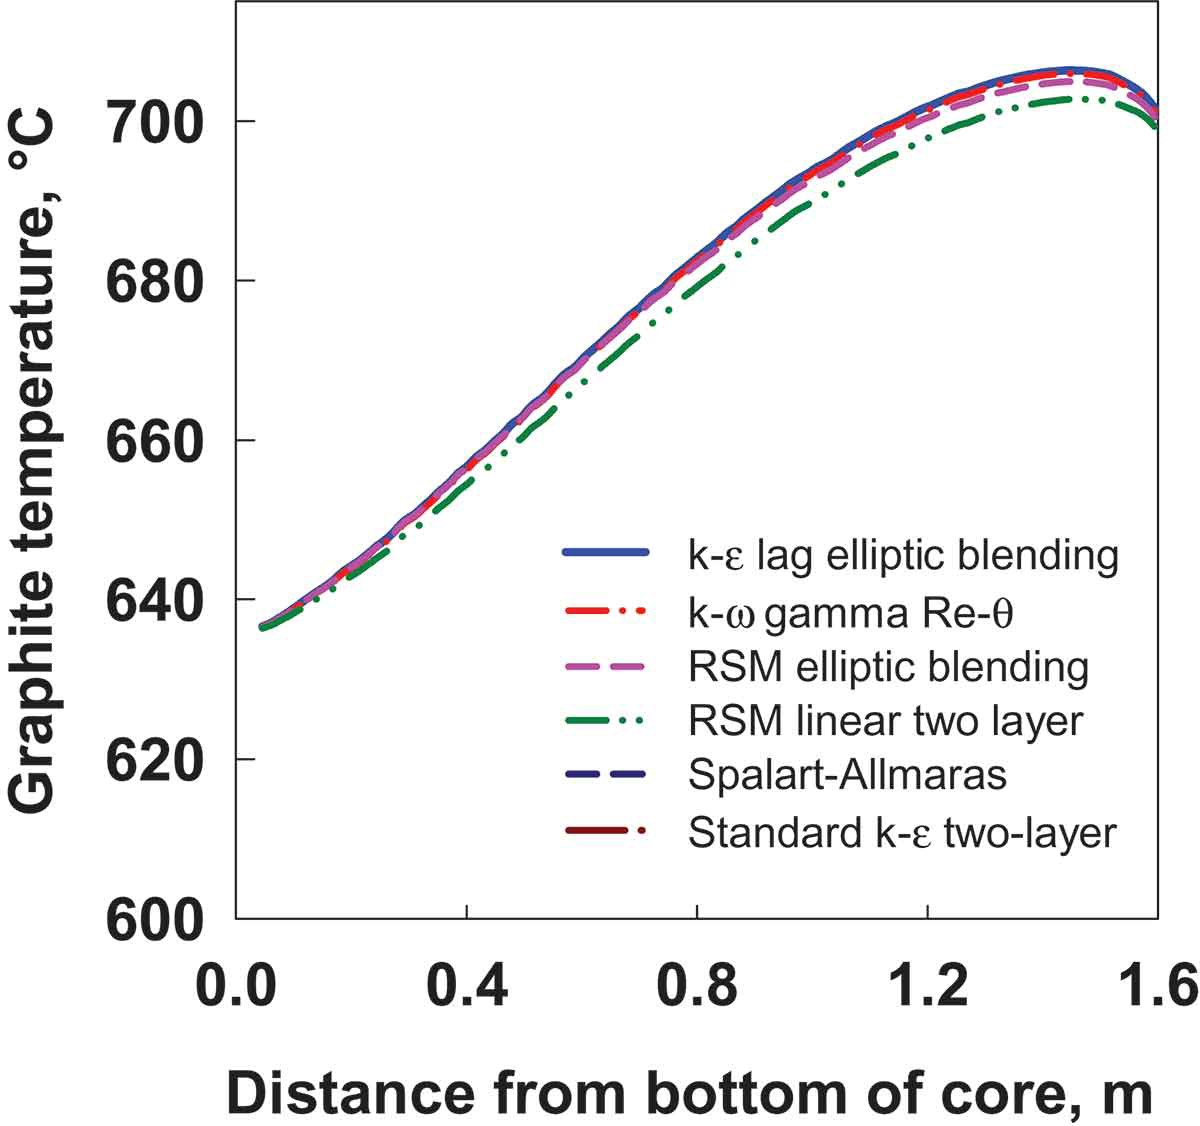
\includegraphics[width=.8\columnwidth]{images/podila-graphite}
    \caption{Graphite temperature adjacent to the hottest MSRE channel.}
  \end{figure}
  \column[t]{5.5cm}
  \begin{figure}
    \centering
    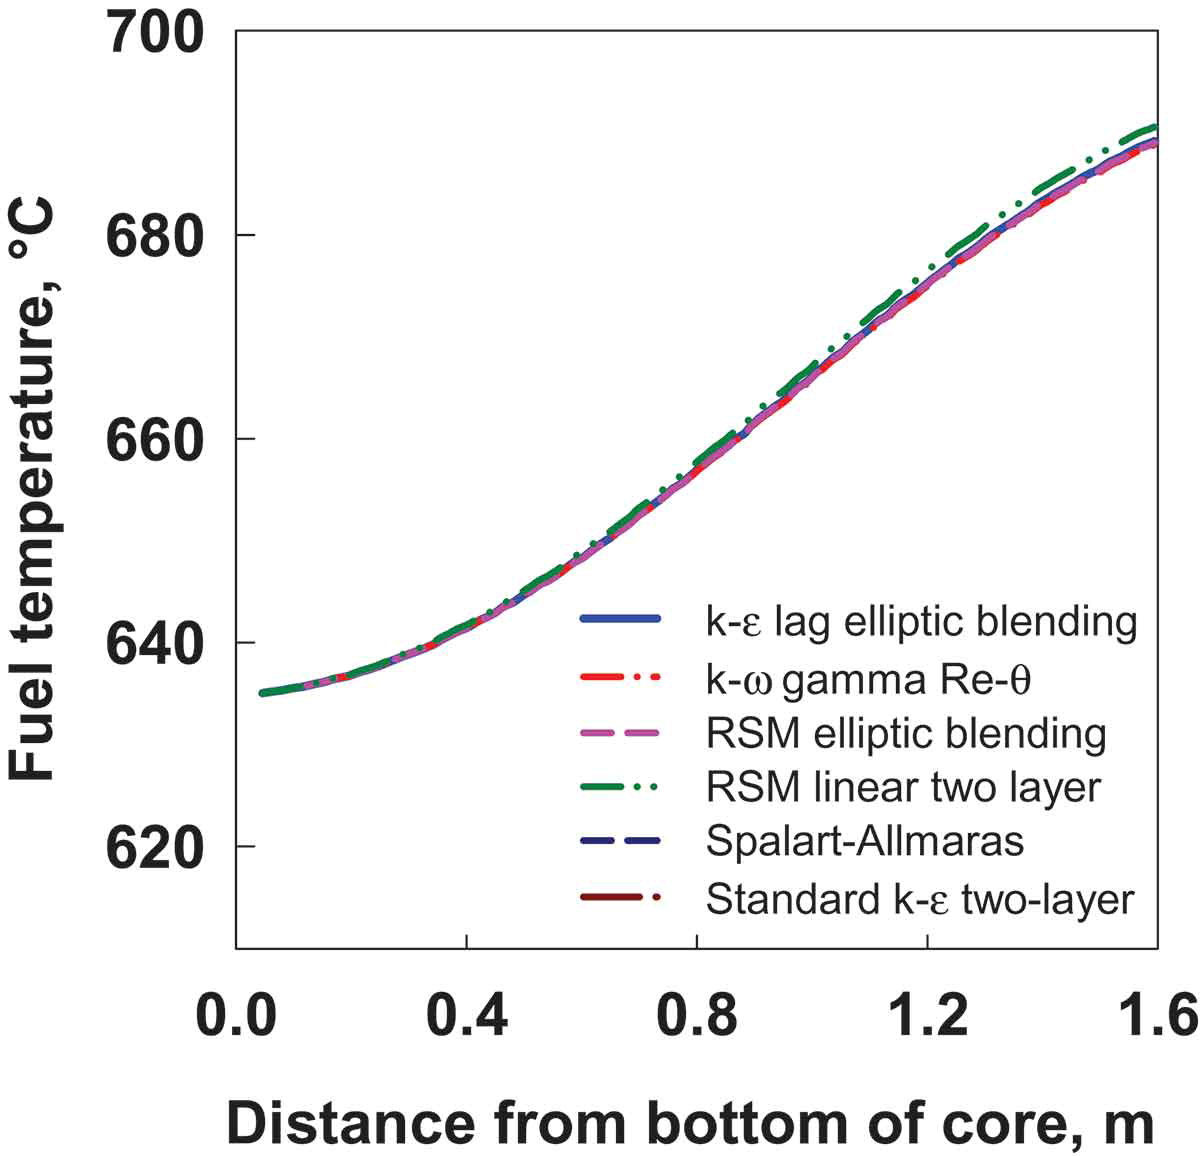
\includegraphics[width=.8\columnwidth]{images/podila-fuel}
    \caption{Fuel temperature in the hottest MSRE channel.}
  \end{figure}
\end{columns}
\end{frame}

\subsection{Proposed Work}
\begin{frame}
  \frametitle{Proposed Work}
  \begin{block}{Implementation of a Spalart-Allmaras turbulence model in Moltres}
    \begin{itemize}
      \item Implement a Spalart-Allmaras model in Moltres
      \item Verify and validate the model against published data for backward-facing step problem
      \item Verify the model against published data of turbulent salt flow in the Molten Salt Fast
        Reactor
    \end{itemize}
  \end{block}
\end{frame}


\section{Objective 3: Hybrid $S_N$-Diffusion Method}
\subsection{Motivation}
\begin{frame}
  \frametitle{Hybrid $S_N$-Diffusion Method: Motivation}
  \begin{columns}
    \hfill
    \column[t]{5cm}
    \textbf{Control Rods in MSRs}
    \vspace{.2cm}
    \begin{figure}
      \centering
      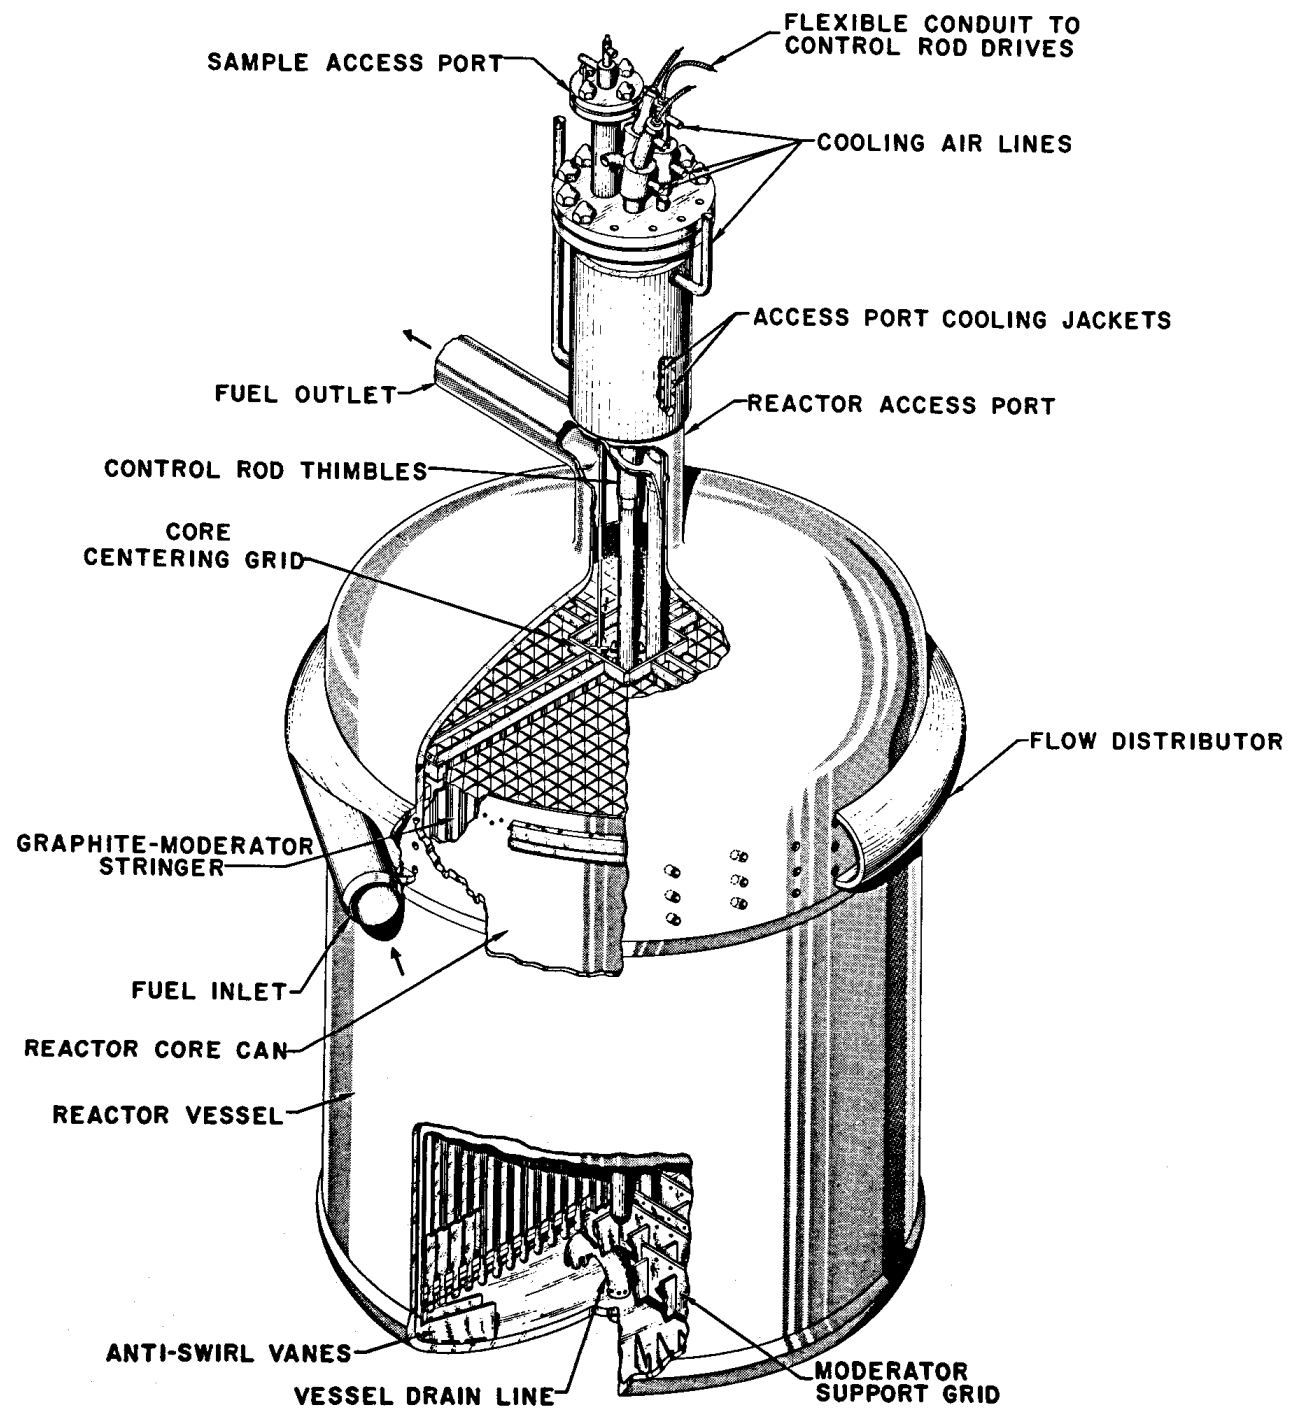
\includegraphics[width=\columnwidth]{images/msre-cutout}
      \caption{\footnotesize MSRE reactor vessel \cite{robertson_msre_1965}}
    \end{figure}
    \hfill
    \column[t]{6cm}
    \begin{figure}
      \centering
      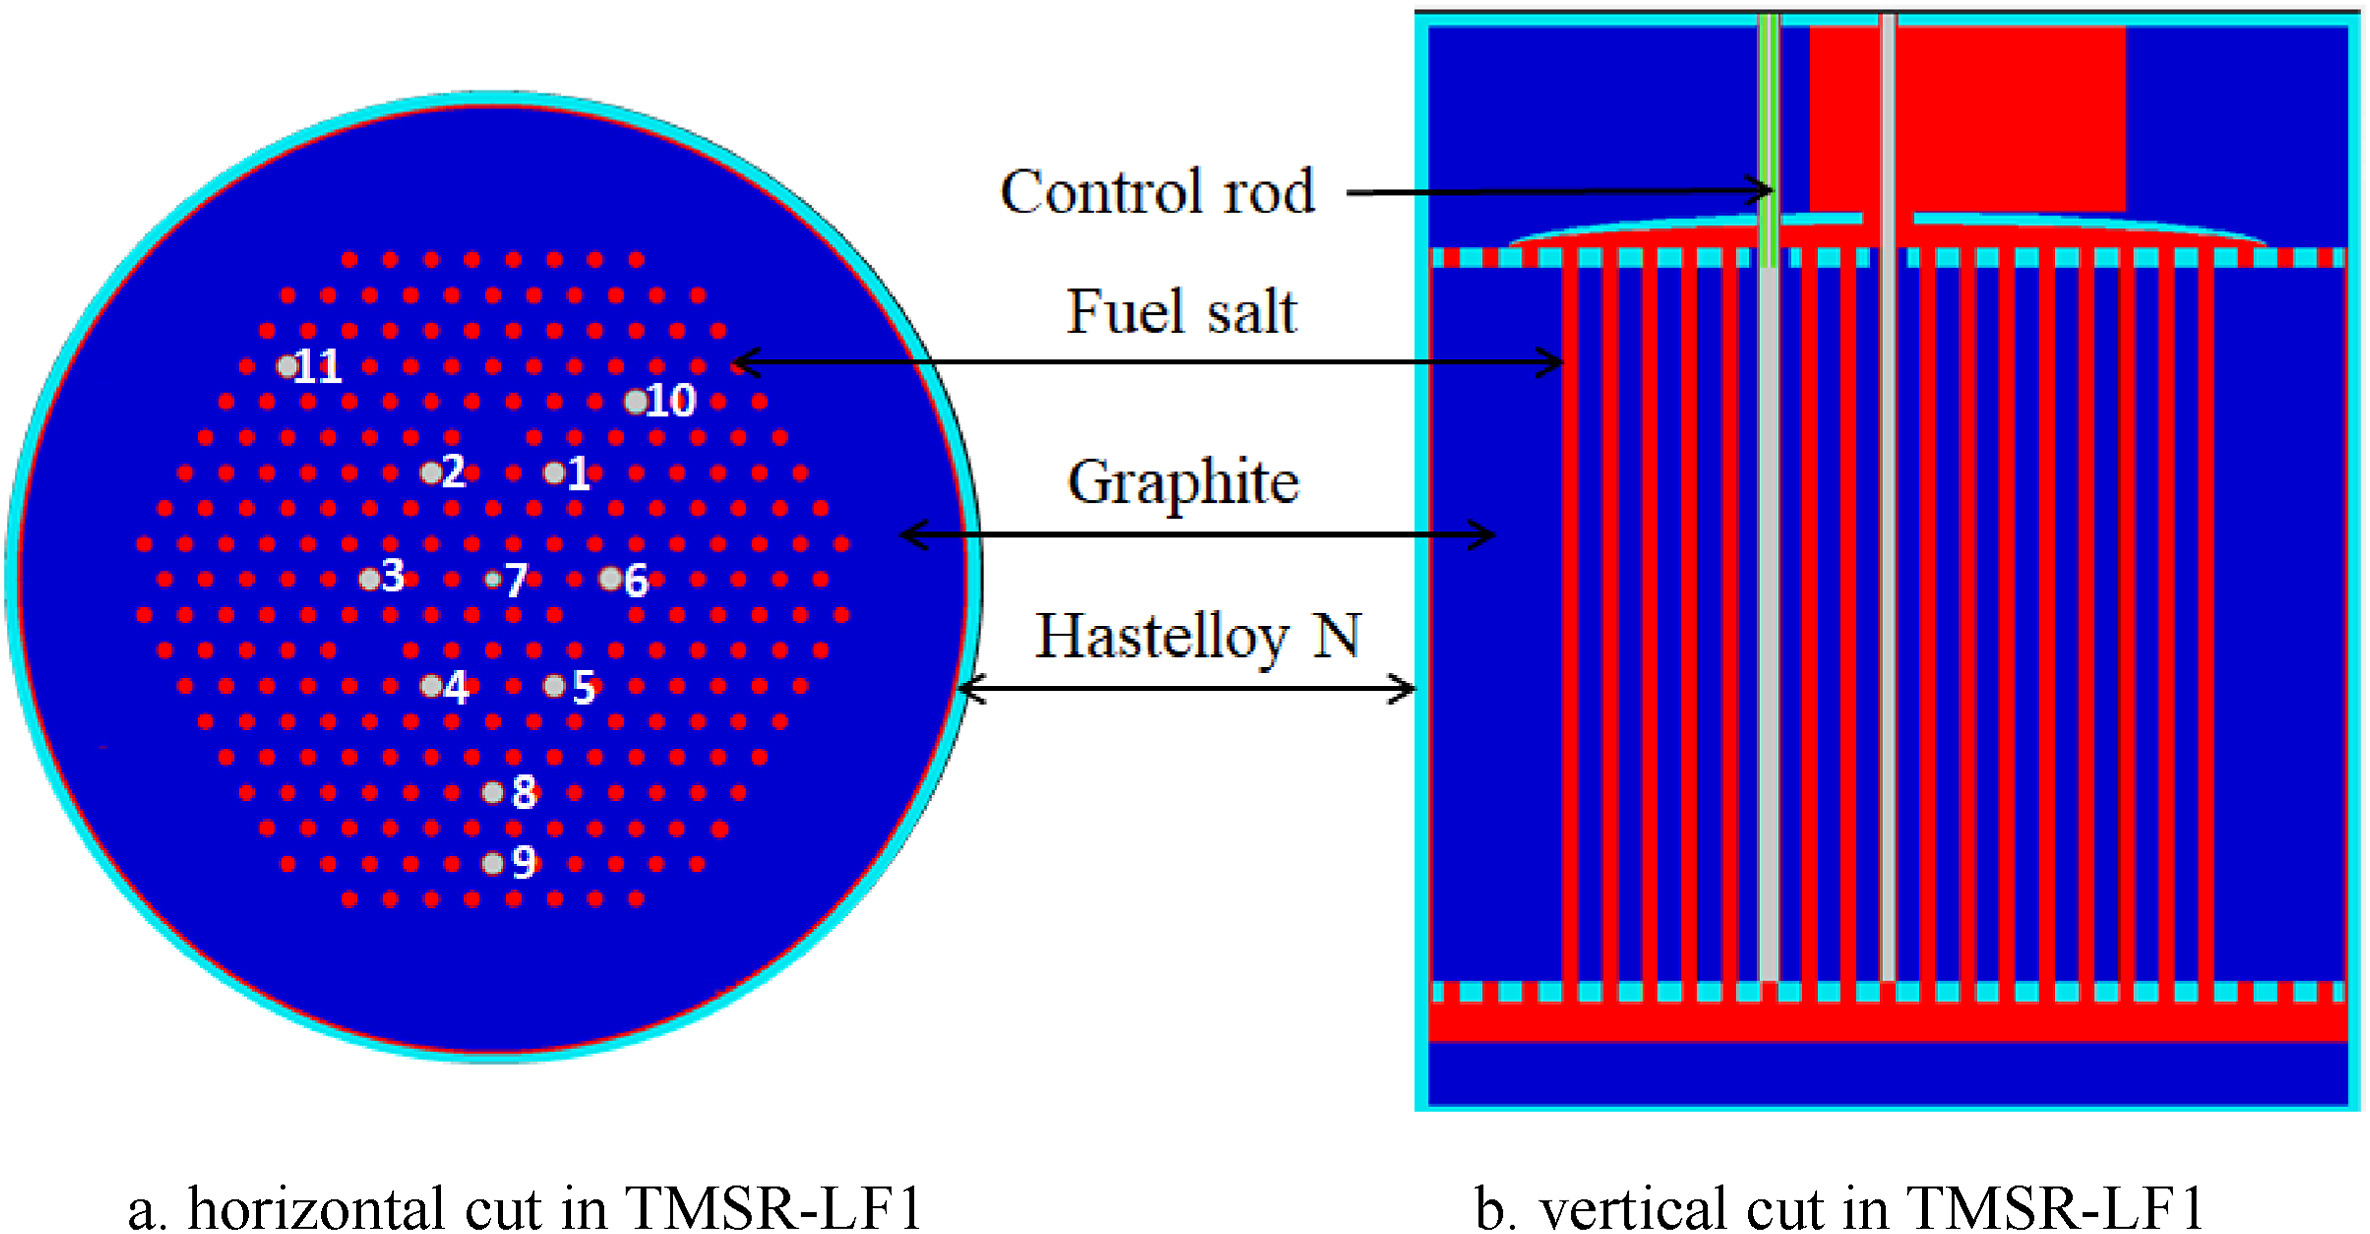
\includegraphics[width=.8\columnwidth]{images/tmsr}
      \caption{\footnotesize Cross-sectional views of the TMSR-LF1
      \cite{liu_sensitivityuncertainty_2020}}
    \end{figure}
    \begin{figure}
      \centering
      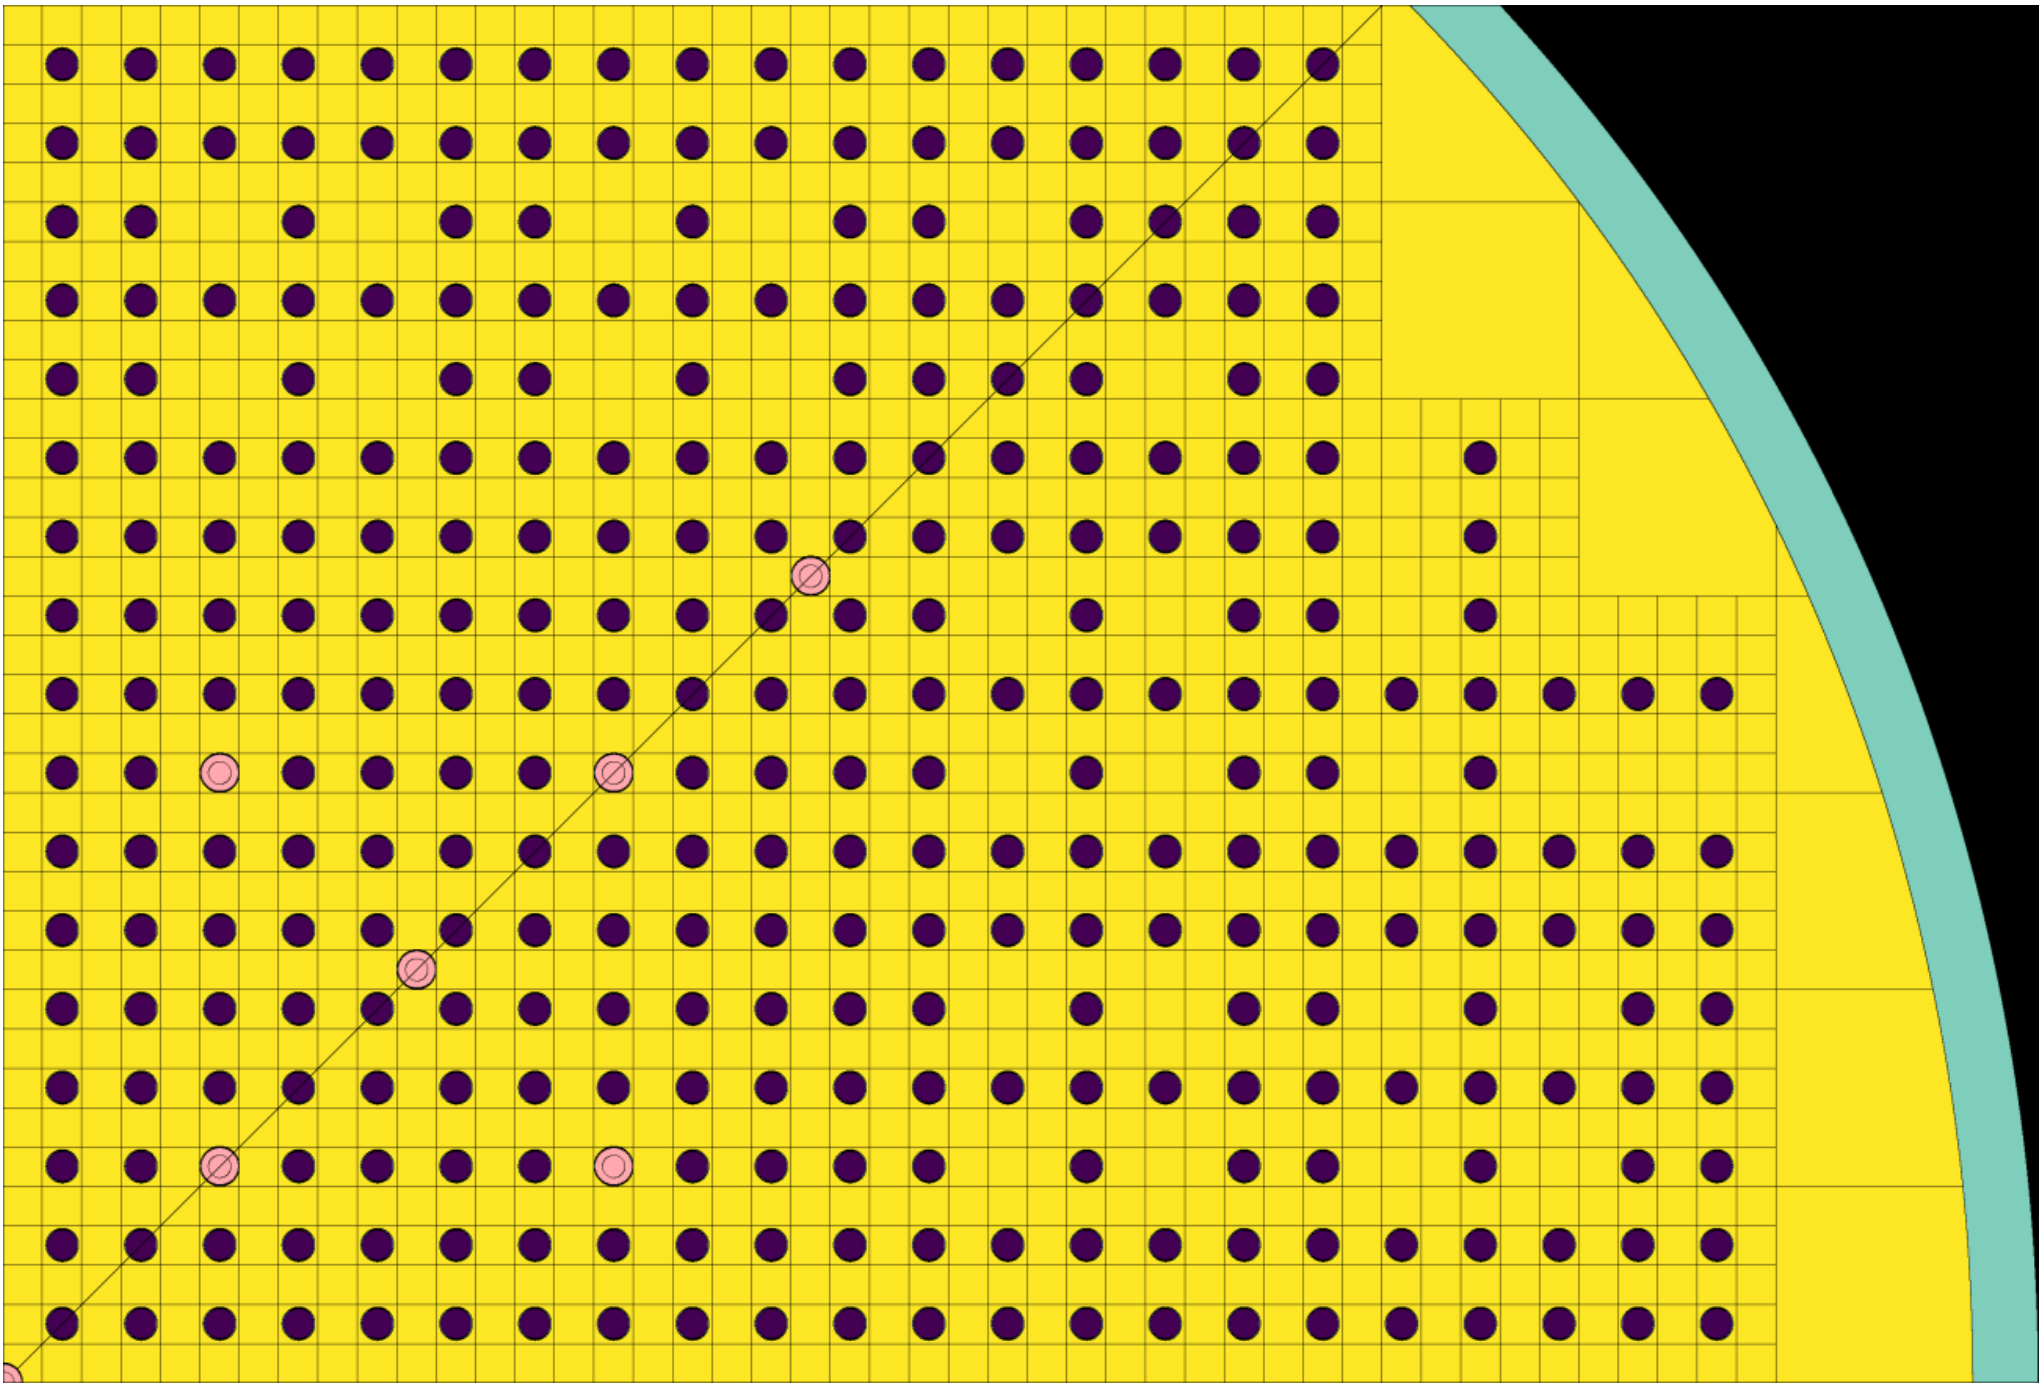
\includegraphics[width=.5\columnwidth]{images/tap-msr-rods}
      \caption{\footnotesize Cross-sectional view of the TAP MSR \cite{lee_neutronics_2020}}
    \end{figure}
    \hfill
  \end{columns}
\end{frame}

\begin{frame}
  \frametitle{Hybrid $S_N$-Diffusion Method: Motivation}
  \textbf{Control rods provide a means of controlling the fission rate in nuclear reactors.} 
  \begin{itemize}
    \item Facilitate reactor start-up, shut-down, or load-following operations
    \item Consist of highly neutron-absorbing materials such as boron or gadolinium
  \end{itemize}
  \textbf{MSRs contain comparatively fewer control rods than most other reactor types due to:}
  \begin{itemize}
    \item Uniform liquid fuel burnup
    \item Strong passive safety of the liquid fuel form
    \item Low excess reactivity of fuel inventory
    \item Availability of other control mechanisms
  \end{itemize}
  \pause
  \textbf{Nevertheless, it is important to characterize control rod effects in all relevant
  transient scenarios.}
\end{frame}

\begin{frame}
  \frametitle{Hybrid $S_N$-Diffusion Method: Motivation}
  \textbf{Control rods induce highly anisotropic neutron fluxes and steep flux gradients in their
  vicinity.}
  \begin{block}{\textbf{The Control Rod Modeling Dilemma}}
    \begin{itemize}
      \item Neutron diffusion, $P_1$, and $SP_N$ methods perform poorly near control rod regions
        due to the highly anisotropic neutron fluxes and steep flux gradients
      \item High-fidelity neutron transport methods remain too computationally expensive for
        routine time-dependent multiphysics simulations
    \end{itemize}
  \end{block}
\end{frame}

\begin{frame}
  \frametitle{Hybrid $S_N$-Diffusion Method: Motivation}
  \textbf{Control Rod Modeling in MSR Multiphysics Studies}
  \vspace{.2cm}

  Common simplifications applied to control rod modeling include:
  \begin{itemize}
    \item Homogenized, coarse-mesh geometries containing static control rods with albedo neutron
      flux boundary conditions \cite{kophazi_development_2009} or transport-corrected cross
      sections \cite{cui_development_2021, jaradat_development_2021, yang_development_2022}
      \begin{itemize}
        \item Neutronics mesh differs from thermal-hydraulics mesh
        \item 1-D thermal-hydraulics model with uniform or prescribed heat deposition
      \end{itemize}
    \item Scaling the neutron source term to simulate moving control rods
      \cite{delpech_benchmark_2003, krepel_dyn3d-msr_2007, jaradat_development_2021,
      yang_development_2022}
      \begin{itemize}
        \item Does not capture local or asymmetric flux changes
      \end{itemize}
  \end{itemize}

  \begin{block}{\textbf{Technical Gap}}
    \textbf{There are no existing MSR simulation tools or studies involving moving control rods
    which are explicitly modeled.}
  \end{block}
\end{frame}

\subsection{Literature Review}
\begin{frame}
  \frametitle{Hybrid $S_N$-Diffusion Method: Literature Review}
  \textbf{Transport-Correction Techniques For Neutron Diffusion-Based Solvers}
  \vspace{.3cm}

  Techniques for augmenting the neutron diffusion method with corrections derived from neutron
  transport
  \begin{itemize}
    \item Absorber Blackness
    \item Method of Equivalent Cross Sections (MECS)
    \item Response-Based Methods
    \item Ronen Method
    \item Transport-Corrected Diffusion Theory
    \item General Equivalence Theory (GET)
    \item Superhomogenization Method (SPH)
  \end{itemize}
  \pause
  \textbf{In this presentation, I will cover the Ronen method and the transport-corrected diffusion
  theory because they are the most similar to my approach.}
\end{frame}

\begin{frame}
  \frametitle{Hybrid $S_N$-Diffusion Method: Literature Review}
  \textbf{The Ronen Method \cite{ronen_accurate_2004}}
  \vspace{.2cm}

  Starting with an initial neutron diffusion flux solution, a transport
  expression is used to iteratively improve the flux solution by updating the
  diffusion coefficients:
  %
  \begin{align}
    D(\vec{r},E) =& -\frac{J_{tr}(\vec{r},E)}{\nabla \phi(\vec{r},E)}
    \label{eq:ronen}
    \shortintertext{where}
    J_{tr} =& \mbox{ transport-derived neutron current.} \nonumber
  \end{align}
  %
  In 1-D slab geometry, the integral expression for calculating the current is:
  %
  \begin{align}
    J(x,E) = \frac{1}{2}\int^a_0 dx'\ &E_2[\tau(x',x,E)sgn(x-x')q_0(x',E) \nonumber \\
    &+\frac{3}{2}\int^a_0dx' \ E_3[\tau(x',x,E)]q_1(x',E)
  \end{align}
  \textbf{Limitation: Demonstrated for 1-D geometries only.}
\end{frame}

\begin{frame}
  \frametitle{Hybrid $S_N$-Diffusion Method: Literature Review}
  \textbf{Transport-Corrected Diffusion Theory \cite{pounders_diffusion_2009}}
  \vspace{.2cm}
  
  Pounders \& Rahnema developed two separate methods which also
  generate space-dependent diffusion coefficients for transport corrections.
  \vspace{.1cm}
  \begin{columns}
    \column[t]{.5\textwidth}
    \textbf{1) Averaged Eddington Factor Diffusion Theory}
    %
    \begin{align}
      \small
      E_g(z) =& \frac{\int^1_{-1} \mu^2\psi(z,\mu)d\mu}{\int^1_{-1} \psi(z,\mu)d\mu}
    \end{align}
    %
    \begin{align}
      \small
      D^{AEF}_g(z) =& E^i_g\left[\hat{\Sigma}_{t,g}-\sum^G_{g'=1}\hat{\Sigma}^{g'\rightarrow g}_{s1}
      \frac{\hat{J}_{g'}}{\hat{J}_g}\right]^{-1}
    \end{align}
    \hfill
    \column[t]{.5\textwidth}
    \textbf{2) High-Order Empirical Diffusion Coefficients}
    \begin{align}
      D^i_g =& -\frac{\left(z_{i+1}-z_i\right) \bar{J}_g}{\left[\phi_g(z_{i+1})-\phi_g(z_i)\right]}
      \label{eq:emp}
    \end{align}
  \end{columns}
  \textbf{Limitation: Both methods require a priori knowledge of the neutron flux and current
  solution.}
\end{frame}

\begin{frame}
  \frametitle{Hybrid $S_N$-Diffusion Method: Literature Review}
  \begin{block}{\textbf{Summary}}
    \begin{itemize}
      \item Demonstrations of the Ronen method are limited to 1-D geometries due to the difficulty of
        deriving transport operators for complex 2-D and 3-D geometries
      \item The transport-corrected diffusion theories by Pounders \& Rahnema require a priori
        knowledge of the neutron flux and current solution
      \item However, their work showed that transport-derived space-dependent diffusion
        coefficients are effective tools applying transport corrections to the neutron diffusion
        equation
    \end{itemize}
  \end{block}
\end{frame}

\subsection{Theory}
\begin{frame}
  \frametitle{Hybrid $S_N$-Diffusion Method: Theory}
  \begin{block}{\textbf{New Method for Improved Control Rod Modeling with Neutron Diffusion}}
    \textbf{Hybrid $\bm{S_N}$-Diffusion Method}
    \begin{itemize}
      \item Applies the discrete ordinates ($S_N$) method to a smaller subregion around a
        control rod to generate corrections for the neutron diffusion equation
      \item Limits computationally expensive $S_N$ calculations to small subdomains
      \item Retains the computational efficiency of the neutron diffusion method
    \end{itemize}
  \end{block}
\end{frame}

\begin{frame}
  \frametitle{Hybrid $S_N$-Diffusion Method: Theory}
  \textbf{1-D Discrete Ordinates $\bm{S_N}$ Equation}
  \begin{align}
    \mu_n \frac{d}{dx}&\Psi_g(x, \mu_n) + \Sigma_{t,g}(x)\Psi_g(x, \mu_n) \nonumber \\
                      &=\sum^G_{g'=1} \sum^N_{n'=1} \sum^L_{l=0}
                        \frac{\left(2l+1\right)}{2} \Sigma^{g'\rightarrow g}_{s,l}(x)
                        P_l(\mu_{n'} - \mu_n) w_{n'}\Psi_{g'}(x,\mu_{n'}) \nonumber \\
                      &\qquad + \sum^G_{g'=1} \frac{\chi_g}{2}
                        \frac{\nu\Sigma_{f,g'}(x)}{k} \phi_{g'}(x) + S_g(x,\mu_n)
    \label{eq:1d-sn}
  \end{align}
  \textbf{1-D Neutron Diffusion Equation}
  \begin{align}
    -\frac{d}{dx} D_g(x) \frac{d}{dx} \phi_g(x) + \Sigma_{t,g}(x) \phi_g(x) = \sum^G_{g'=1}&\left[
      \Sigma_s^{g'\rightarrow g}(x)\phi_{g'}(x) + \chi_g\frac{\nu\Sigma_{f,g'}(x)}{k}
    \phi_{g'}(x)\right] \nonumber \\
                                   &+ S_g(x)
    \label{eq:1d-diff}
  \end{align}
\end{frame}

\begin{frame}
  \frametitle{Hybrid $S_N$-Diffusion Method: Theory}
  \textbf{Spatially Varying Diffusion Coefficients (SVDCs)}
  \vspace{.3cm}

  Transport corrections are in the form of \textit{Spatially Varying Diffusion Coefficients
  (SVDCs)}:
  %
  \begin{align}
    D^s_g(x) &= -J^{tr}_g(x)\bigg/\frac{d\phi^{tr}_g(x)}{dx}. \label{eq:svdc}
  \end{align}
  %
  where $D^s$ is the \glspl{SVDC}, and the $tr$ superscript denotes neutron
  current and scalar flux computed from the $S_N$ method. This formulation is similar to the
  space-dependent diffusion coefficients for the Ronen method.
\end{frame}

\begin{frame}
  \frametitle{Hybrid $S_N$-Diffusion Method: Theory}
  \begin{columns}
    \column{.35\textwidth}
    \textbf{Hybrid $S_N$-Diffusion Method Algorithm}
    \vspace{.5cm}

  {\small
  $V_0$: Full problem domain
  \vspace{.1cm}

  $V_1$: Problem subdomain containing control rod region
  \vspace{.1cm}

  $D^s_i$: SVDCs in the $i$-th iteration
\vspace{4cm}}
  \column{.65\textwidth}
  \begin{figure}
    \centering
    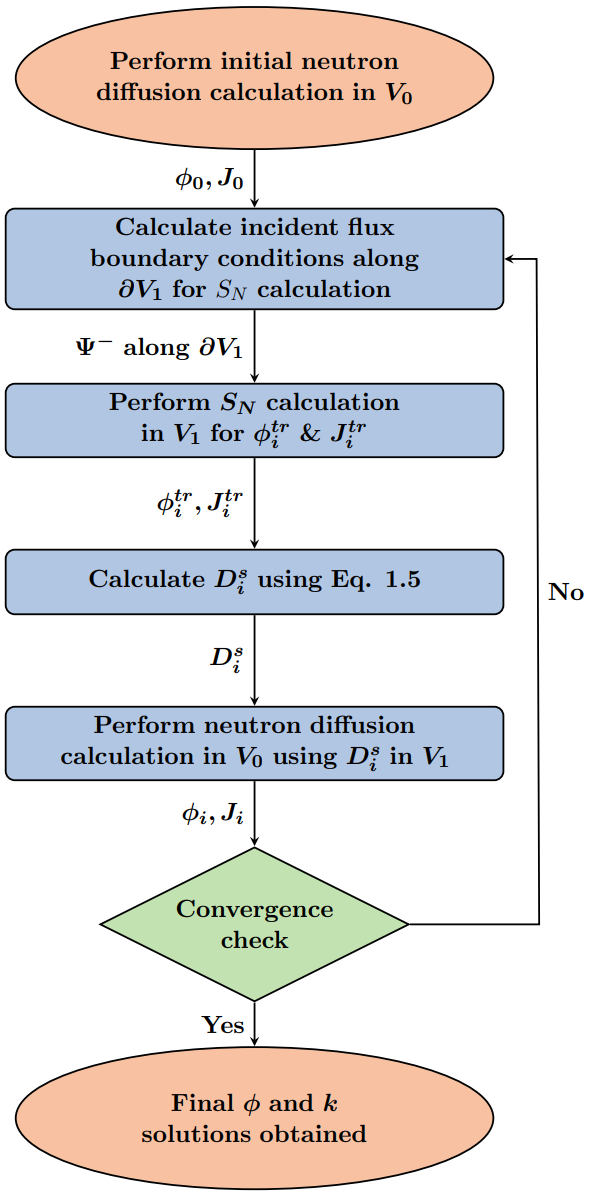
\includegraphics[width=.49\textwidth]{images/algorithm}
    \begin{minipage}[b]{.49\textwidth}
      \caption{Algorithm flowchart for the hybrid $S_N$-diffusion method.}
    \end{minipage}
  \end{figure}
\end{columns}
\end{frame}

\begin{frame}
  \frametitle{Hybrid $S_N$-Diffusion Method: Theory}
  \textbf{$S_N$ Subsolver Boundary Conditions}
  \vspace{.3cm}
  \begin{itemize}
    \item In 1-D, the $S_N$ method requires $N/2$ boundary flux parameters per mesh point.
    \item However, the neutron diffusion method can produce at most one independent parameter per
      mesh point.
    %
    \begin{align}
      J_{g,\pm} &= \frac{\phi_g}{4} \mp \frac{D_g}{2}\frac{d\phi_g}{dx} \label{eq:p1-j}
      \shortintertext{where}
      J_{g,\pm} &= \mbox{ neutron forward/backward current of group }g. \nonumber
    \end{align}
    %
  \end{itemize}
  \pause
  $\Rightarrow$ Assume uniformly isotropic transmission of angular flux:
  %
  \begin{align}
    \Psi_g(x,\mu_n) =& J_{g,+}(x)\Bigg/\sum^N_{n=N/2+1}w_n\mu_n && (\mu_n>0) \\
    \Psi_g(x,\mu_n) =& J_{g,-}(x)\Bigg/\sum^{N/2}_{n=1}w_n\mu_n && (\mu_n<0)
  \end{align}
\end{frame}

\begin{frame}
  \frametitle{Hybrid $S_N$-Diffusion Method: Theory}
  \textbf{Correction Region ($\bm{V_1}$) and Buffer Zone}
  \begin{itemize}
    \item Recall that the full problem domain and the correction region are defined as $V_0$
      and $V_1$, where $V_1 \subseteq V_0$
    \item The approximate $S_N$ boundary conditions will generally yield some deviations in the
      flux distribution since neutron fluxes in realistic reactor systems are at least slightly
      anisotropic in most of the system
    \item However, the influence of boundary conditions on the ratio of $J$ and $\frac{d\phi}{dx}$
      does not extend far from the boundary $\partial V_1$ in optically thick media; SVDCs are
      accurate everywhere except near $\partial V_1$
  \end{itemize}
  \pause
  $\Rightarrow$ Approach for preliminary results: Define $V_1$ such that it is large enough to
  provide sufficient transport
  corrections and accommodate inaccurate SVDCs near $\partial V_1$. Discard inaccurate SVDCs
  in favor of the default $P_1$-based diffusion coefficients.
\end{frame}


\subsection{Preliminary Results}
\begin{frame}
  \frametitle{Hybrid $S_N$-Diffusion Method: Preliminary Results}
  \textbf{Illustration of the Hybrid Method With Case 0} \\
  \begin{columns}
    \column[t]{5.5cm}
    \textbf{Problem Description}
    \begin{itemize}
      \item 1-D, two-region system consisting of:
      \begin{itemize}
        \item 0.5-cm thick control rod region
        \item 19.5-cm thick homogenized mixture of molten fuel salt and graphite moderator
      \end{itemize}
      \item Material compositions from the Molten Salt Reactor Experiment (MSRE)
      \item Two-group constants are sampled at 900 K and generated using OpenMC
    \end{itemize}
    \column[t]{5.5cm}
    \begin{figure}[htb!]
      \centering
      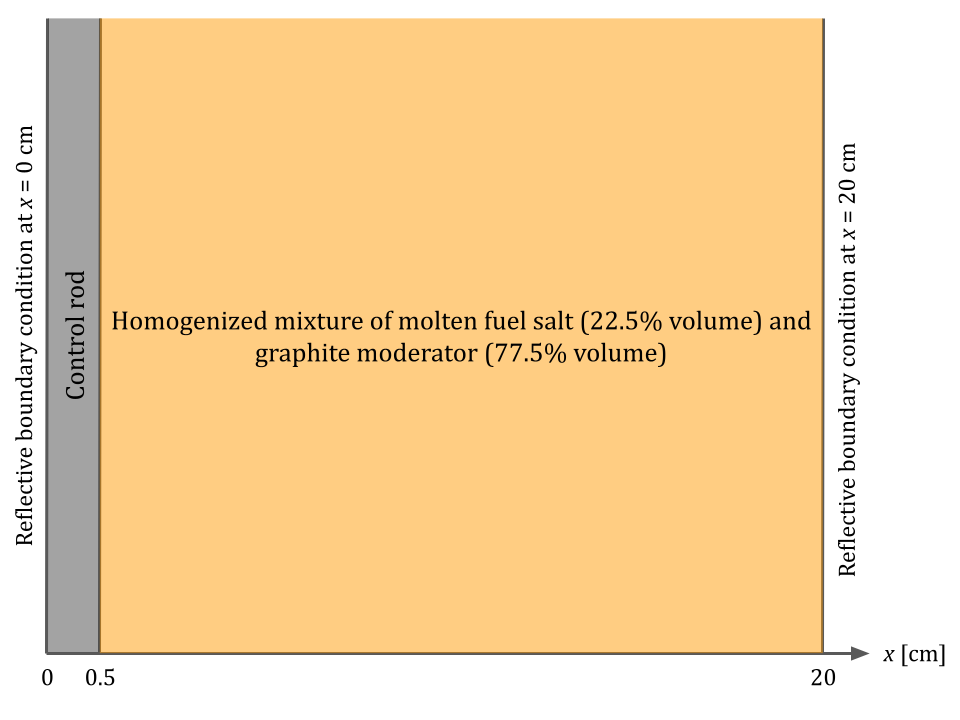
\includegraphics[width=\columnwidth]{../images/case-0-geometry}
      \caption{Case 0 problem geometry.}
      \label{fig:case-0-geom}
    \end{figure}
  \end{columns}
\end{frame}

\begin{frame}
  \frametitle{Hybrid $S_N$-Diffusion Method: Preliminary Results}
  \textbf{Illustration of the Hybrid Method With Case 0}
  \vspace{.3cm}

  I solved for the neutron flux in Case 0 using the following set of numerical solvers:
  \begin{enumerate}
    \item Neutron diffusion solver with $P_1$-based diffusion coefficients generated directly from
      the group constants generation step with OpenMC
    \item $S_N$ neutron transport solver with $N=8$ and up to 2nd-order anisotropic scattering
      cross sections
    \item Neutron diffusion solver with SVDCs generated from the prior $S_8$ flux solution
    \item Hybrid $S_N$-Diffusion solver with $\Omega^d_1$ spanning from $x=0$ cm to $x=17.5$ cm
  \end{enumerate}

  The neutron diffusion and $S_N$ solvers are implemented in Python using the finite difference
  method and diamond difference method, respectively.
\end{frame}

\begin{frame}
  \frametitle{Hybrid $S_N$-Diffusion Method: Preliminary Results}
  \textbf{Case 0 Results}
  \begin{figure}
    \centering
    \begin{subfigure}[b]{.49\textwidth}
      \centering
      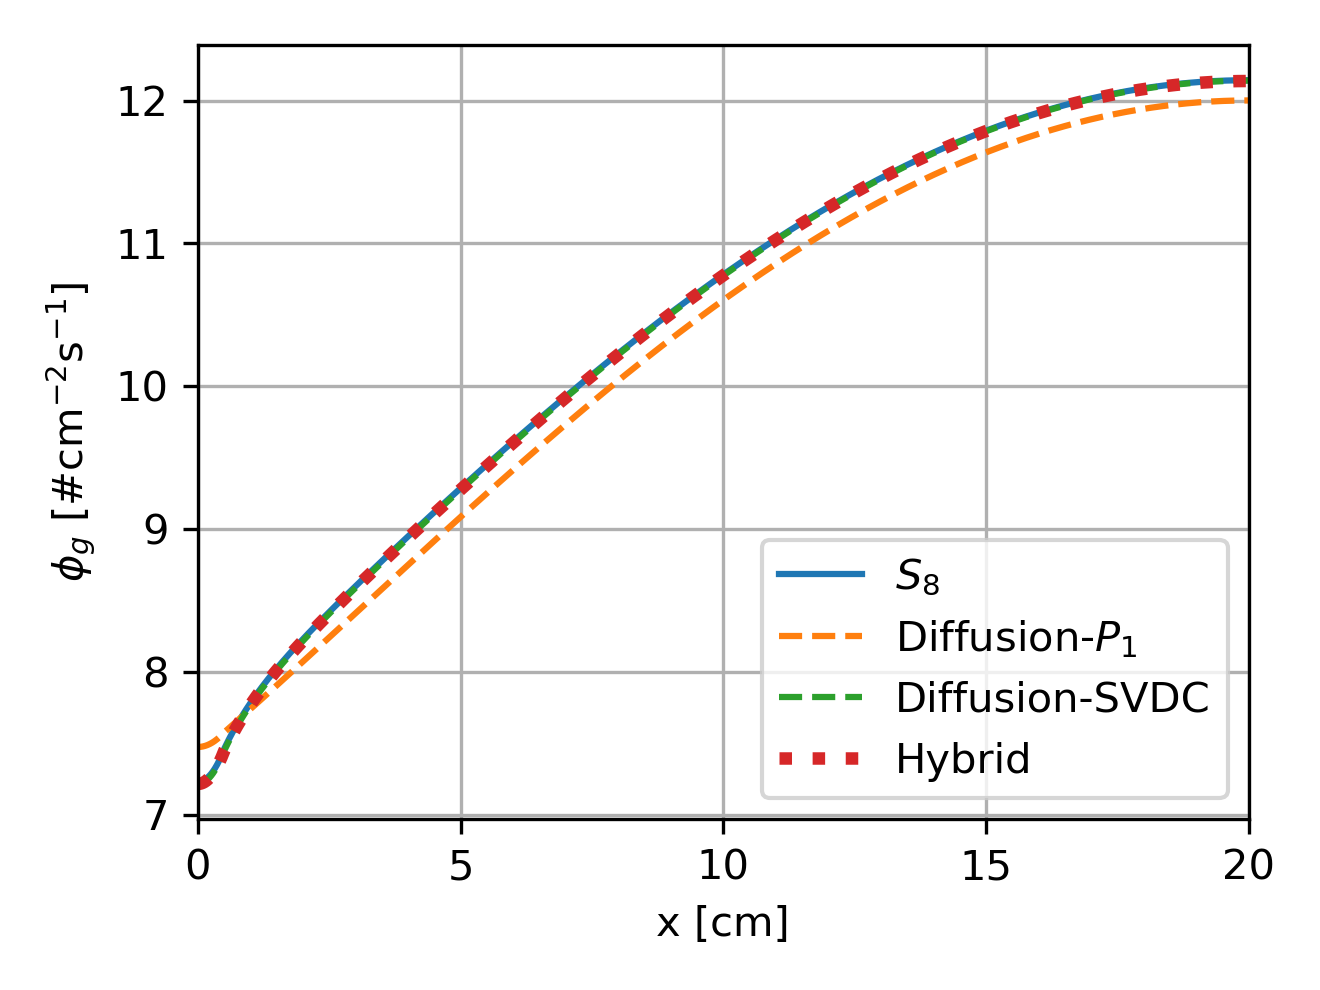
\includegraphics[width=\textwidth]{../images/case-0-group-1-hybrid-flux}
      \caption{Group 1}
      \label{fig:c0g1hf}
    \end{subfigure}
    \hfill
    \begin{subfigure}[b]{.49\textwidth}
      \centering
      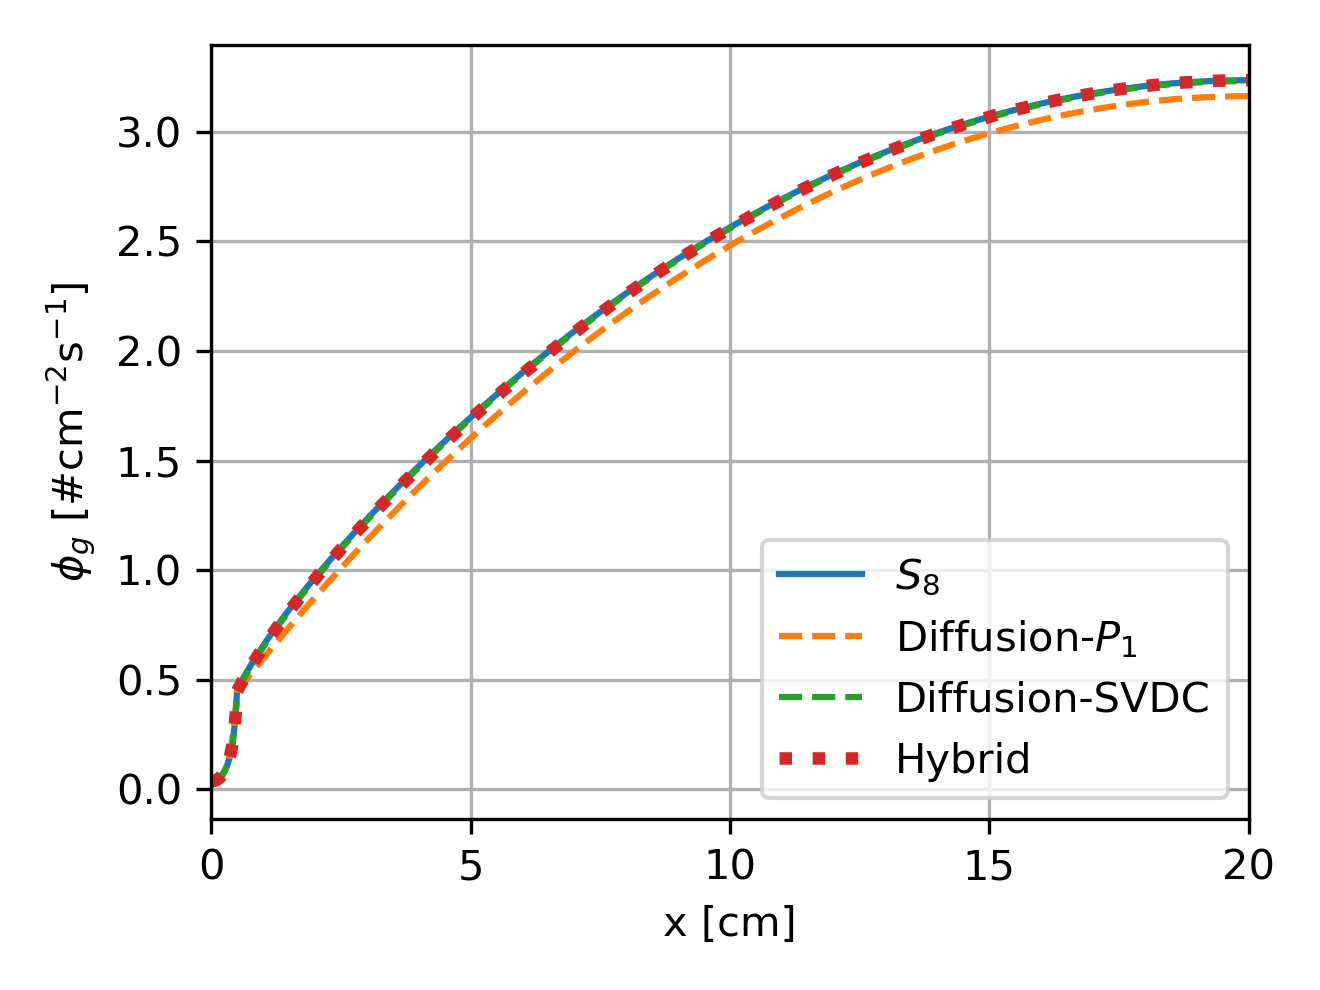
\includegraphics[width=\textwidth]{../images/case-0-group-2-hybrid-flux}
      \caption{Group 2}
      \label{fig:c0g2hf}
    \end{subfigure}
    \caption{Neutron group 1 and 2 flux distributions from the diffusion, $S_8$, reference
    \gls{SVDC}, and hybrid methods for Case 0.}
  \end{figure}
\end{frame}

\begin{frame}
  \frametitle{Hybrid $S_N$-Diffusion Method: Preliminary Results}
  \textbf{Case 0 Results}
  \begin{figure}
    \centering
    \begin{subfigure}[b]{.49\textwidth}
      \centering
      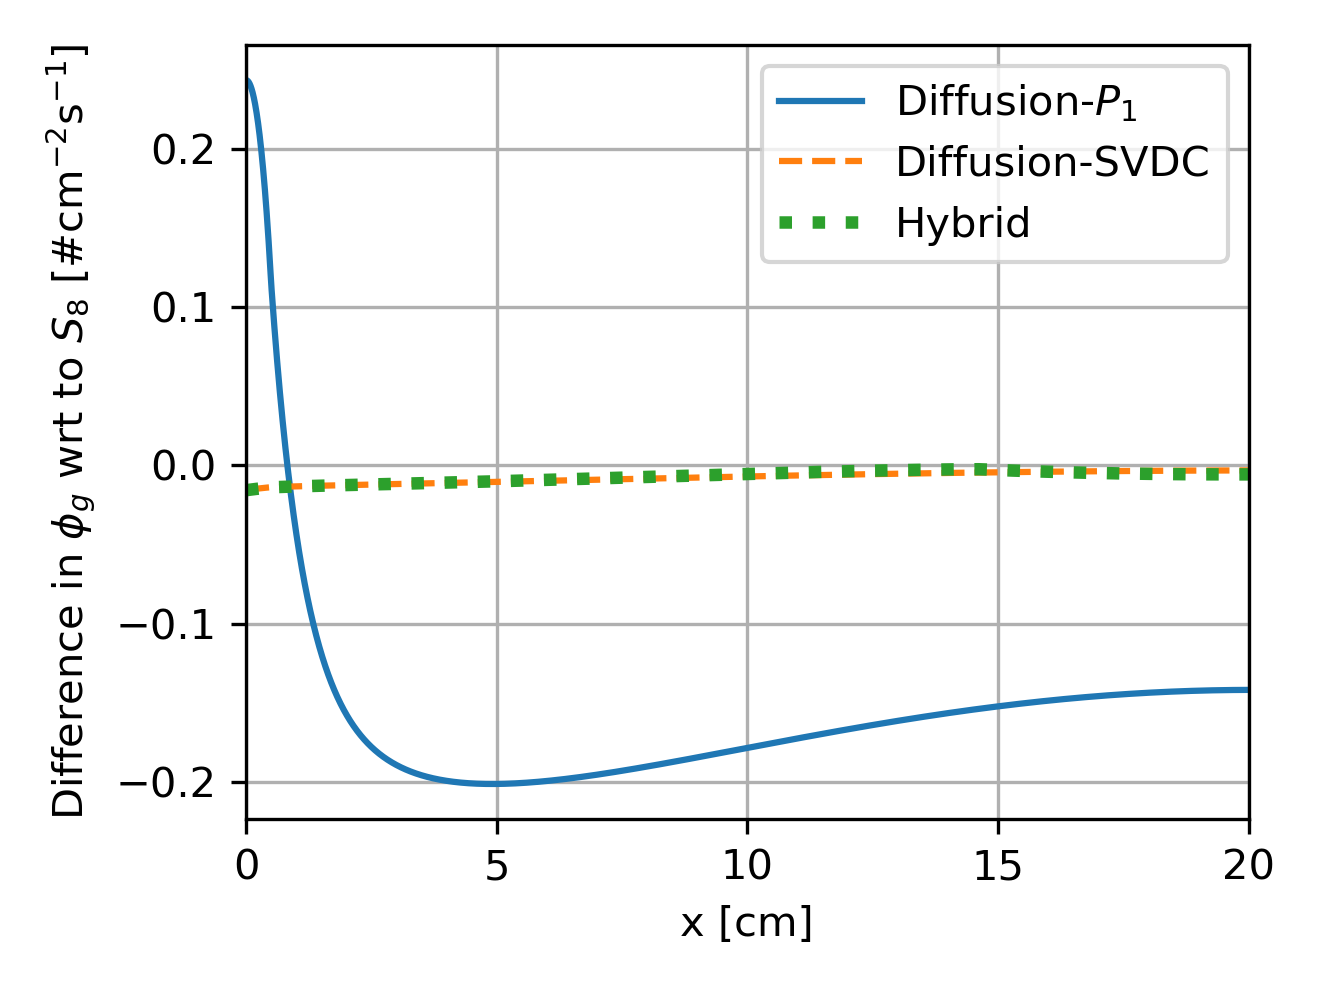
\includegraphics[width=\textwidth]{../images/case-0-group-1-hybrid-flux-diff}
      \caption{Group 1}
      \label{fig:c0g1hfdiff}
    \end{subfigure}
    \hfill
    \begin{subfigure}[b]{.49\textwidth}
      \centering
      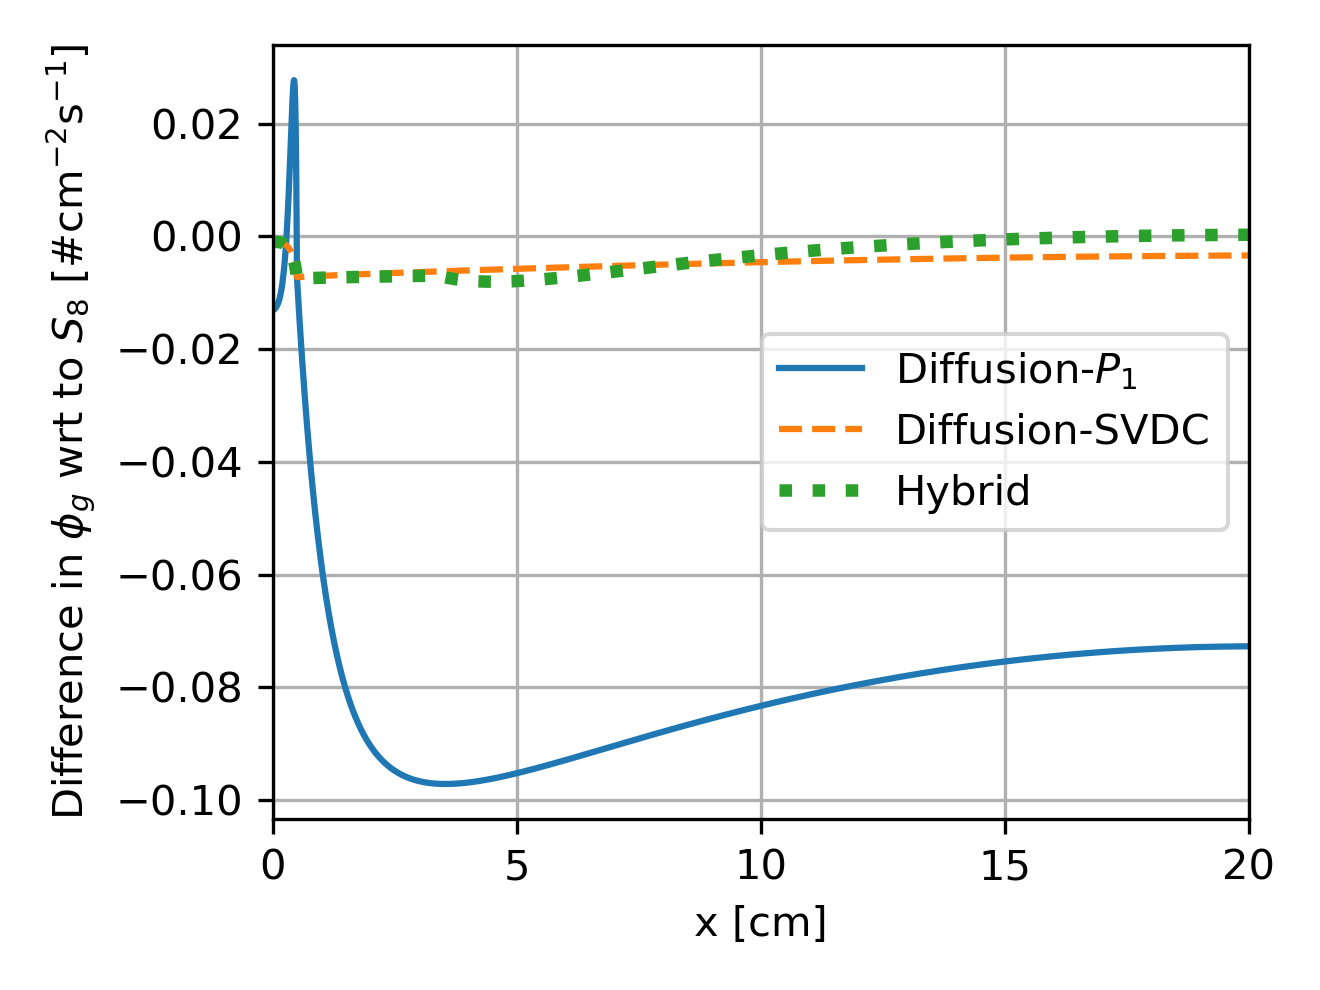
\includegraphics[width=\textwidth]{../images/case-0-group-2-hybrid-flux-diff}
      \caption{Group 2}
      \label{fig:c0g2hfdiff}
    \end{subfigure}
    \caption{Difference in neutron group 1 and 2 flux distributions from the diffusion,
    diffusion-\gls{SVDC}, and hybrid methods with respect to the $S_8$ flux distribution for Case 0.}
    \label{fig:c0hfdiff}
  \end{figure}
\end{frame}

\begin{frame}
  \frametitle{Hybrid $S_N$-Diffusion Method: Preliminary Results}
  \textbf{Case 0 Results}
  \begin{table}
    \centering
    \caption{Multiplication factor $k$ estimates from the diffusion-$P_1$, $S_8$, and
    diffusion-\gls{SVDC} solvers and the absolute difference relative to the $S_8$ estimate.}
    \begin{tabular}{l S S}
      \toprule
      Solver type & {$k$} & {$k-k_{S8}$} \\
      \midrule
      $S_8$ & 0.62736 & {-} \\
      Diffusion-$P_1$ & 0.60890 & -0.01846 \\
      Diffusion-\gls{SVDC} & 0.62750 & +0.00013 \\
      Hybrid & 0.62774 & +0.00038 \\
      \bottomrule
    \end{tabular}
    \label{table:c0k}
  \end{table}
\end{frame}

\begin{frame}
  \frametitle{Hybrid $S_N$-Diffusion Method: Preliminary Results}
  \textbf{Case 0 Results}
  \begin{figure}[htb!]
    \centering
    \begin{subfigure}[b]{.49\textwidth}
      \centering
      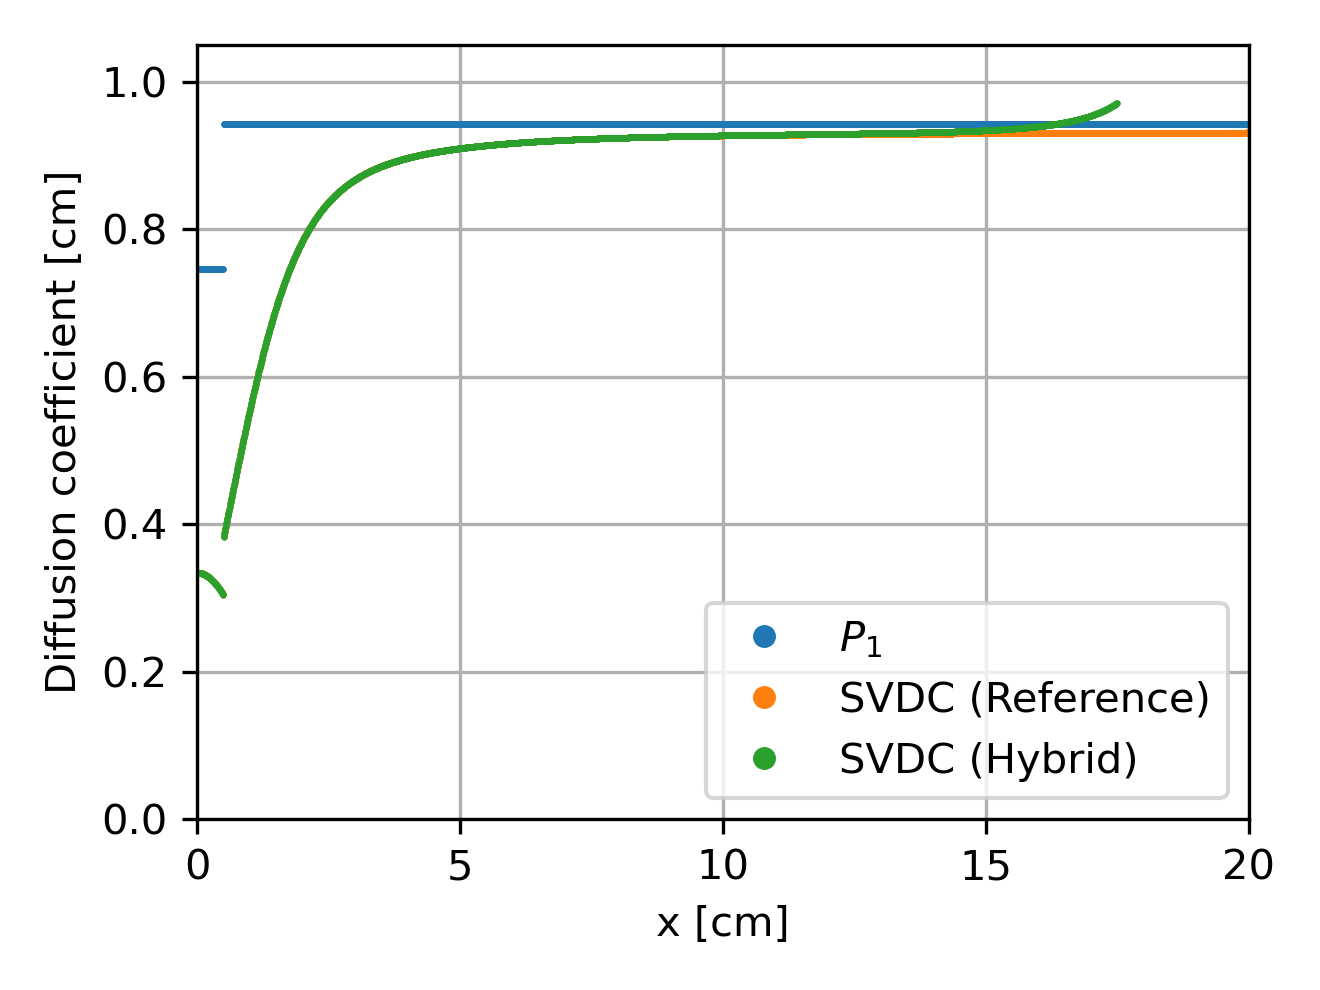
\includegraphics[width=\textwidth]{../images/case-0-group-1-hybrid-diffcoef}
      \caption{Group 1}
      \label{fig:c0g1hd}
    \end{subfigure}
    \hfill
    \begin{subfigure}[b]{.49\textwidth}
      \centering
      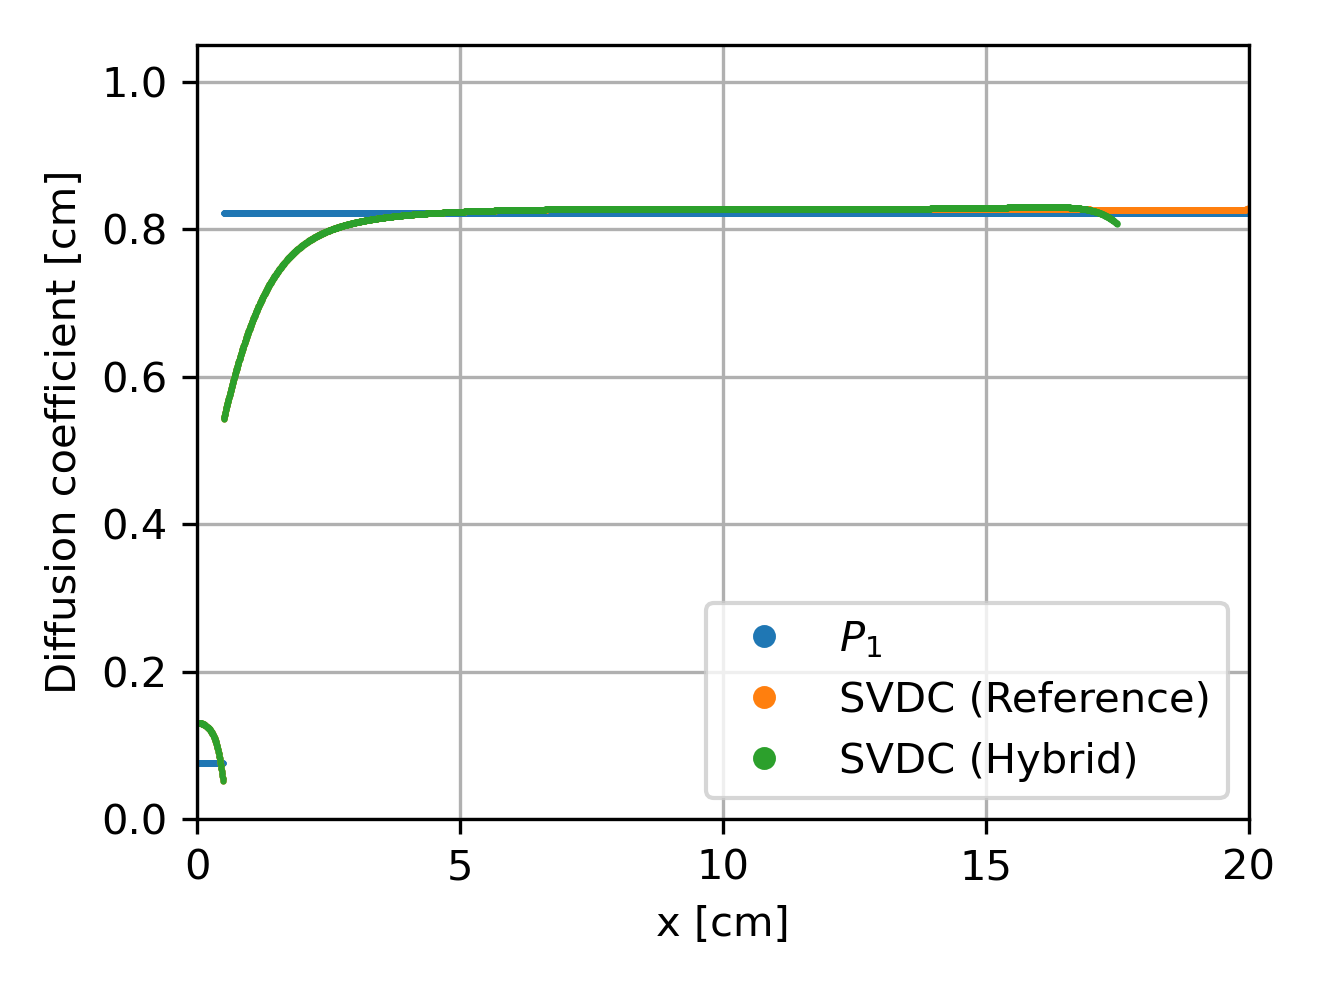
\includegraphics[width=\textwidth]{../images/case-0-group-2-hybrid-diffcoef}
      \caption{Group 2}
      \label{fig:c0g2hd}
    \end{subfigure}
    \caption{$P_1$-based flux-limited diffusion coefficient and \gls{SVDC} spatial distribution for
    Case 0. The \gls{SVDC} distributions were generated from the reference $S_8$ (``SVDC'') and the
    hybrid (``Hybrid'') calculations.}
    \label{fig:c0hd}
  \end{figure}
\end{frame}

\begin{frame}
  \frametitle{Hybrid $S_N$-Diffusion Method: Preliminary Results}
  \textbf{Case 0 Discussion}
  \begin{itemize}
    \item The hybrid method automatically determines the buffer zone size by comparing the SVDCs
      to the $P_1$ diffusion coefficient values.
    \item The hybrid method converges rapidly within two outer iterations.
    \item The required size of $\Omega^d_1$ for Case 0 is large because the control rod region is
      the only significant source of influence on the neutron flux.
    \item $\Omega^d_1$ is smaller for more realistic reactor systems which are more heterogeneous
      and have vacuum boundary conditions.
  \end{itemize}
\end{frame}

\begin{frame}
  \frametitle{Hybrid $S_N$-Diffusion Method: Preliminary Results}
  \textbf{Further 1-D Test Cases}
  \begin{figure}[htb!]
    \centering
    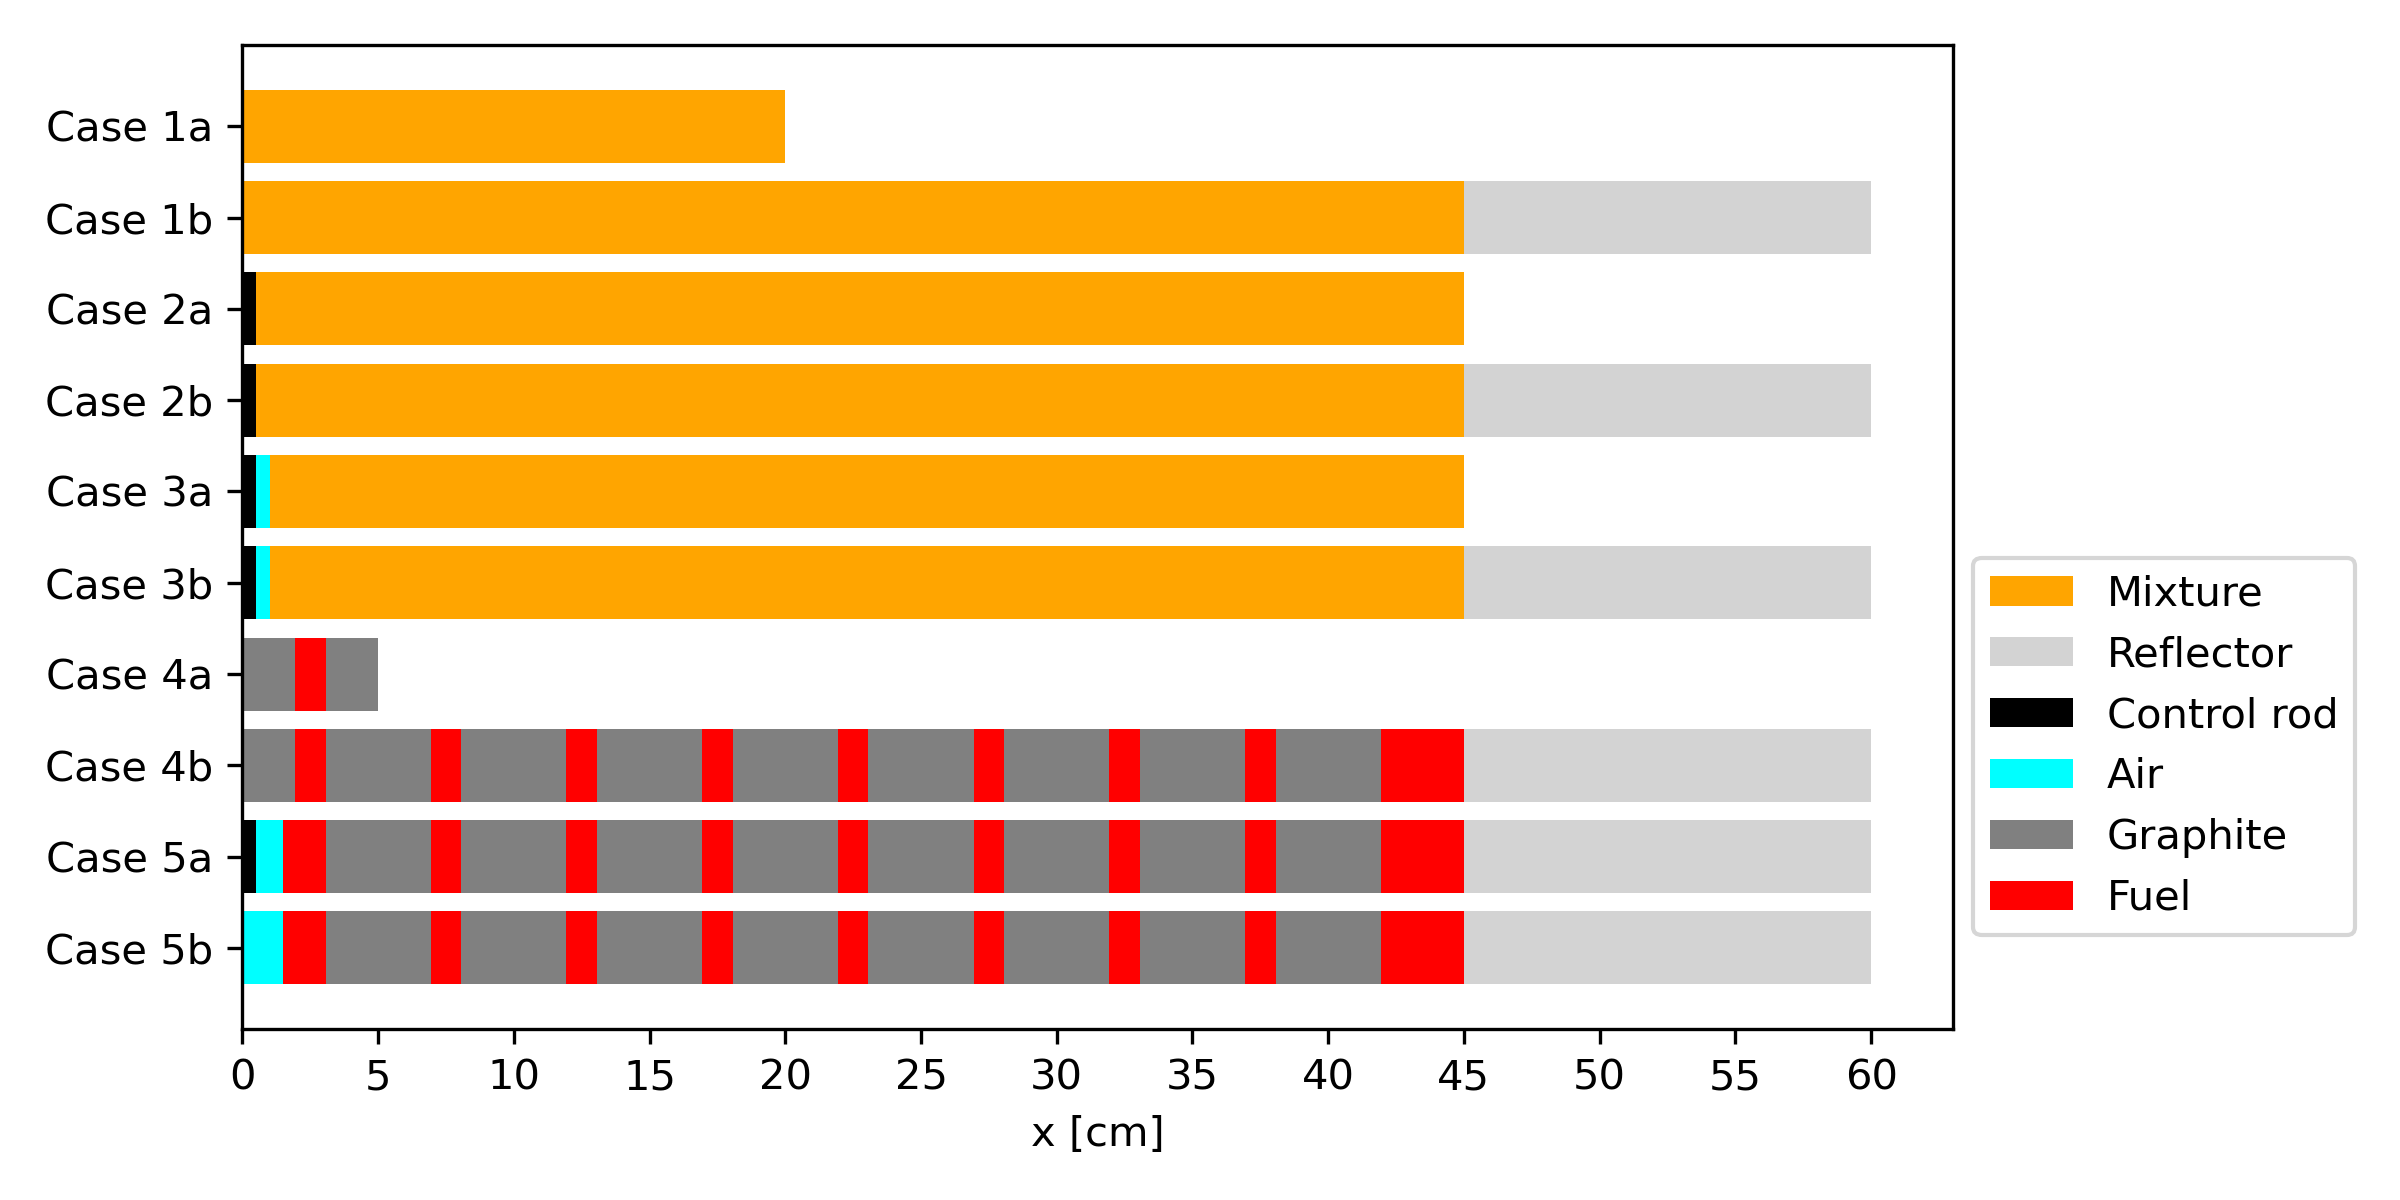
\includegraphics[width=\columnwidth]{../images/case-geometry}
    \caption{Geometries of the 1-D test cases. All geometries
      have reflective boundary conditions on the boundary at $x=0$ cm. The right-side boundaries are
      reflective for Cases 1a, 2a, 3a, and 4a, and vacuum for Cases 1b, 2b, 3b, 4b, 5a, and 5b.}
    \label{fig:case-geom}
  \end{figure}
\end{frame}

\begin{frame}
  \frametitle{Hybrid $S_N$-Diffusion Method: Preliminary Results}
  \textbf{1-D Test Case Problem Setup}
  \begin{itemize}
    \item Material compositions derived from the MSRE design
    \item Four neutron energy groups
      \begin{itemize}
        \item Bounded at $E=10^{-5}, 10^0, 10^2, 10^5, 10^8$ eV
      \end{itemize}
    \item Group constants generated using OpenMC with up to 2nd-order anisotropic scattering
      matrices
  \end{itemize}
  \begin{columns}
    \column{12cm}
  \begin{table}
    \centering
    \scriptsize
    \caption{Variable handling in OpenMC under continuous-energy (OpenMC-CE) and multigroup
    (OpenMC-MG) modes, and in the $S_N$ neutron transport, neutron diffusion, and Hybrid
    $S_N$-Diffusion methods. }
    \begin{tabular}{c c c c c c}
      \toprule
      Variable & OpenMC-CE & OpenMC-MG & $S_N$ Transport & Diffusion & Hybrid \\
      \midrule
      Position, $\bm{r}$ & Continuous & Continuous & Discrete & Discrete & Discrete \\
      Direction of travel, $\bm{\hat{\Omega}}$ & Continuous & Continuous & Discrete & N/A & N/A \\
      Energy, $E$ & Continuous & Discrete & Discrete & Discrete & Discrete \\
      Angle-dependence in $\Sigma_s$ & Continuous & 2nd Legendre moment & 2nd Legendre moment
      & N/A & N/A \\
      \bottomrule
    \end{tabular}
    \label{table:var}
  \end{table}
  \end{columns}
\end{frame}

\begin{frame}
  \frametitle{Hybrid $S_N$-Diffusion Method: Preliminary Results}
  \textbf{Simulation Parameters}
  \begin{table}
    \centering
    \footnotesize
    \caption{Simulation parameters applied to the neutron diffusion, $S_N$, and Hybrid
    $S_N$-Diffusion methods.}
    \begin{tabular}{c c c c}
      \toprule
      Parameter & $S_N$ Transport & Neutron Diffusion & Hybrid $S_N$-Diffusion \\
      \midrule
      Mesh size, $\Delta x$ [cm]        & 0.0125    & 0.0125    & 0.0125 \\[.2cm]
      \multirow{3}{*}{Convergence tolerance, $tol$}
                                        &           &           & Diffusion: $10^{-6}$ \\
                                        & $10^{-7}$ & $10^{-6}$ & $S_N$: $10^{-5}$ \\
                                        &           &           & Outer: $10^{-3}$ \\[.2cm]
      Discrete ordinates, $N$           & 8         & N/A       & 8 \\
      Highest moment of $\Sigma^{g'\rightarrow g}_s$, $L$
                                        & 2         & N/A       & 2 \\
      \bottomrule
    \end{tabular}
    \label{table:param}
  \end{table}
\end{frame}

\begin{frame}
  \frametitle{Hybrid $S_N$-Diffusion Method: Preliminary Results}
  \textbf{Test Case Results}
  \begin{table}
    \centering
    \scriptsize
    \caption{Multiplication factor $k$ estimates for Cases 1a, 1b, 2a, 2b, 3a, and 3b.}
    \begin{tabular}{c S[table-format=1.5(2)] S[table-format=1.5(2)] S[table-format=1.5(2)]
    S[table-format=1.5(2)] S[table-format=1.5(2)] S[table-format=1.5(2)]}
      \toprule
      \multirow{2}{*}{\textbf{Method}} &
      \multicolumn{6}{c}{\textbf{Multiplication factor,} $\bm{k}$} \\
      \cmidrule{2-7}
      & {\textbf{Case 1a}} & {\textbf{Case 1b}} & {\textbf{Case 2a}} &
      {\textbf{Case 2b}} & {\textbf{Case 3a}} & {\textbf{Case 3b}} \\
      \midrule
      OpenMC-CE & 1.60033(56) & 1.16749(60) & 1.20666(66) & 0.69499(47) & 1.19908(63) & 0.68565(53)\\
      OpenMC-MG & 1.60015(33) & 1.18104(54) & 1.20570(66) & 0.70539(50) & 1.19976(48) & 0.69730(50)\\
      $S_8$     & 1.60035     & 1.18068     & 1.20596     & 0.70470     & 1.19968     & 0.69652    \\
      Diffusion & 1.60036     & 1.17932     & 1.19709     & 0.69274     & 1.19064     & 0.68450    \\
      Hybrid    & {N/A}       & {N/A}       & 1.20630     & 0.70387     & 1.20004     & 0.69568    \\
      \bottomrule
    \end{tabular}
    \label{table:ck1}
  \end{table}
  %
  \begin{table}
    \centering
    \scriptsize
    \caption{Multiplication factor $k$ estimates for Cases 4a, 4b, 5a, and 5b.}
    \begin{tabular}{c S[table-format=1.5(2)] S[table-format=1.5(2)] S[table-format=1.5(2)]
      S[table-format=1.5(2)]}
      \toprule
      \multirow{2}{*}{\textbf{Method}} &
      \multicolumn{4}{c}{\textbf{Multiplication factor,} $\bm{k}$} \\
      \cmidrule{2-5}
      & {\textbf{Case 4a}} & {\textbf{Case 4b}} & {\textbf{Case 5a}} &
      {\textbf{Case 5b}} \\
      \midrule
      OpenMC-CE & 1.64506(53) & 1.19116(63) & 0.70352(64) & 1.16832(58) \\
      OpenMC-MG & 1.64355(37) & 1.20738(63) & 0.71396(50) & 1.18204(53) \\
      $S_8$     & 1.64376     & 1.20744     & 0.71379     & 1.18218     \\
      Diffusion & 1.64355     & 1.20811     & 0.70524     & 1.18274     \\
      Hybrid    & {N/A}       & {N/A}       & 0.71673     & {N/A}       \\
      \bottomrule
    \end{tabular}
    \label{table:ck2}
  \end{table}
\end{frame}

\begin{frame}
  \frametitle{Hybrid $S_N$-Diffusion Method: Preliminary Results}
  \textbf{Test Case Results}
  \begin{columns}
    \column{12cm}
  \begin{table}[htb!]
    \centering
    \scriptsize
    \caption{Differences in $k$ estimates for Cases 1a, 1b, 2a, 2b, 3a, and 3b for the $S_8$ neutron
      transport, neutron diffusion, and Hybrid $S_N$-Diffusion methods relative to OpenMC-MG.}
    \begin{tabular}{c S[table-format=+1.5(2)] S[table-format=+1.5(2)] S[table-format=+1.5(2)]
        S[table-format=+1.5(2)] S[table-format=+1.5(2)] S[table-format=+1.5(2)]}
      \toprule
      \multirow{2}{*}{\textbf{Method}} & \multicolumn{6}{c}{$\bm{k-k_{MG}}$} \\
      \cmidrule{2-7}
      & {\textbf{Case 1a}} & {\textbf{Case 1b}} & {\textbf{Case 2a}} &
      {\textbf{Case 2b}} & {\textbf{Case 3a}} & {\textbf{Case 3b}} \\
      \midrule
      $S_8$     & +0.00020(33) & -0.00036(54) & +0.00026(66) & -0.00069(50) & -0.00008(48) & -0.00078(50) \\
      Diffusion & +0.00021(33) & -0.00172(54) & -0.00861(66) & -0.01265(50) & -0.00912(48) & -0.01280(50) \\
      Hybrid    & {N/A}        & {N/A}        & +0.00060(66) & -0.00152(50) & +0.00028(48) & -0.00162(50) \\
      \bottomrule
    \end{tabular}
    \label{table:ckdiff1}
  \end{table}
  %
  \begin{table}[htb!]
    \centering
    \scriptsize
    \caption{Differences in $k$ estimates for Cases 4a, 4b, 5a, and 5b for the $S_8$ neutron
      transport, neutron diffusion, and Hybrid $S_N$-Diffusion methods relative to OpenMC-MG.}
    \begin{tabular}{c S[table-format=+1.5(2)] S[table-format=+1.5(2)] S[table-format=+1.5(2)]
      S[table-format=+1.5(2)]}
      \toprule
      \multirow{2}{*}{\textbf{Method}} & \multicolumn{4}{c}{$\bm{k-k_{MG}}$} \\
      \cmidrule{2-5}
      & {\textbf{Case 4a}} & {\textbf{Case 4b}} & {\textbf{Case 5a}} &
      {\textbf{Case 5b}} \\
      \midrule
      $S_8$     & +0.00021(37) & +0.00006(63) & -0.00017(50) & -0.00027(53) \\
      Diffusion & +0.00000(37) & +0.00073(63) & -0.00872(50) & +0.00277(53) \\
      Hybrid    & {N/A}        & {N/A}        & +0.00070(50) & {N/A}    \\
      \bottomrule
    \end{tabular}
    \label{table:ckdiff2}
  \end{table}
  %
\end{columns}
\end{frame}

\begin{frame}
  \frametitle{Hybrid $S_N$-Diffusion Method: Preliminary Results}
  \textbf{Test Case Results}
  \begin{table}
    \centering
    \footnotesize
    \caption{Control rod worths calculated as changes in the reactivity between Case 5a and 5b for
      the OpenMC continuous-energy and multigroup mode calculations, and the $S_8$ neutron transport,
    neutron diffusion, and Hybrid $S_N$-Diffusion methods.}
    \begin{tabular}{c S}
      \toprule
      \multirow{2}{*}{\textbf{Method}} & {\textbf{Control rod worth}} \\
                                       & {$\bm{\rho_{(5b)}-\rho_{(5a)}}$} \\
      \midrule
      OpenMC-CE & 0.56549(213) \\
      OpenMC-MG & 0.55464(176) \\
      $S_8$     & 0.55507 \\
      Diffusion & 0.57246 \\
      Hybrid    & 0.54974 \\
      \bottomrule
    \end{tabular}
    \label{table:rod-worth}
  \end{table}
  The hybrid method generates improved control rod worth estimates over the standard neutron
  diffusion method.
\end{frame}

\begin{frame}
  \frametitle{Hybrid $S_N$-Diffusion Method: Preliminary Results}
  \begin{columns}
    \column{8cm}
    \begin{figure}
      \centering
      \begin{subfigure}[t]{.45\textwidth}
        \centering
        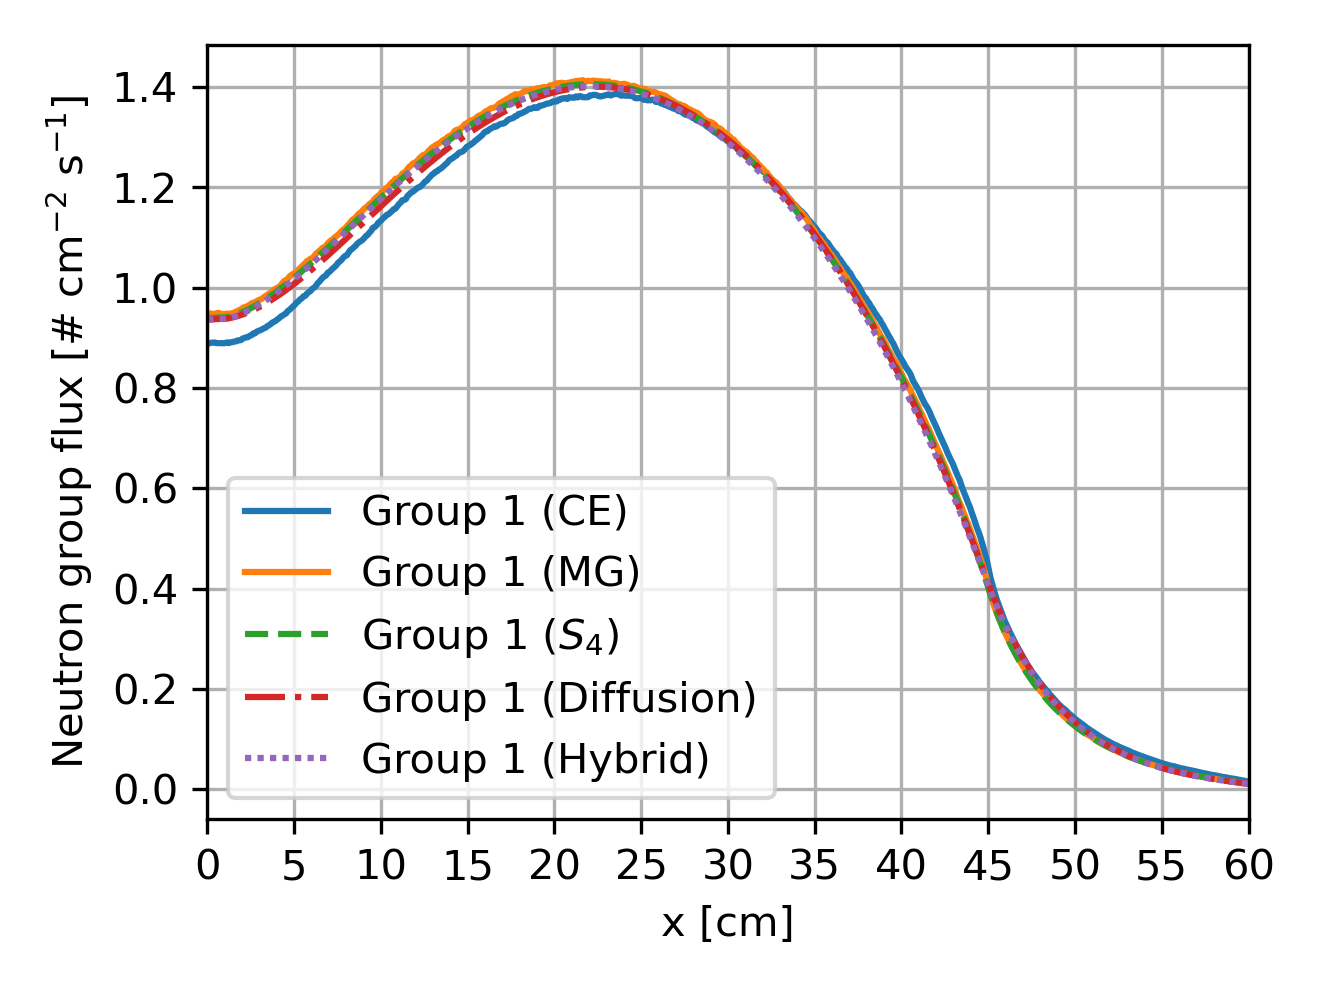
\includegraphics[width=\textwidth]{../images/case-3b-group-1-flux}
        \label{fig:c3bg1}
      \end{subfigure}
      \begin{subfigure}[t]{.45\textwidth}
        \centering
        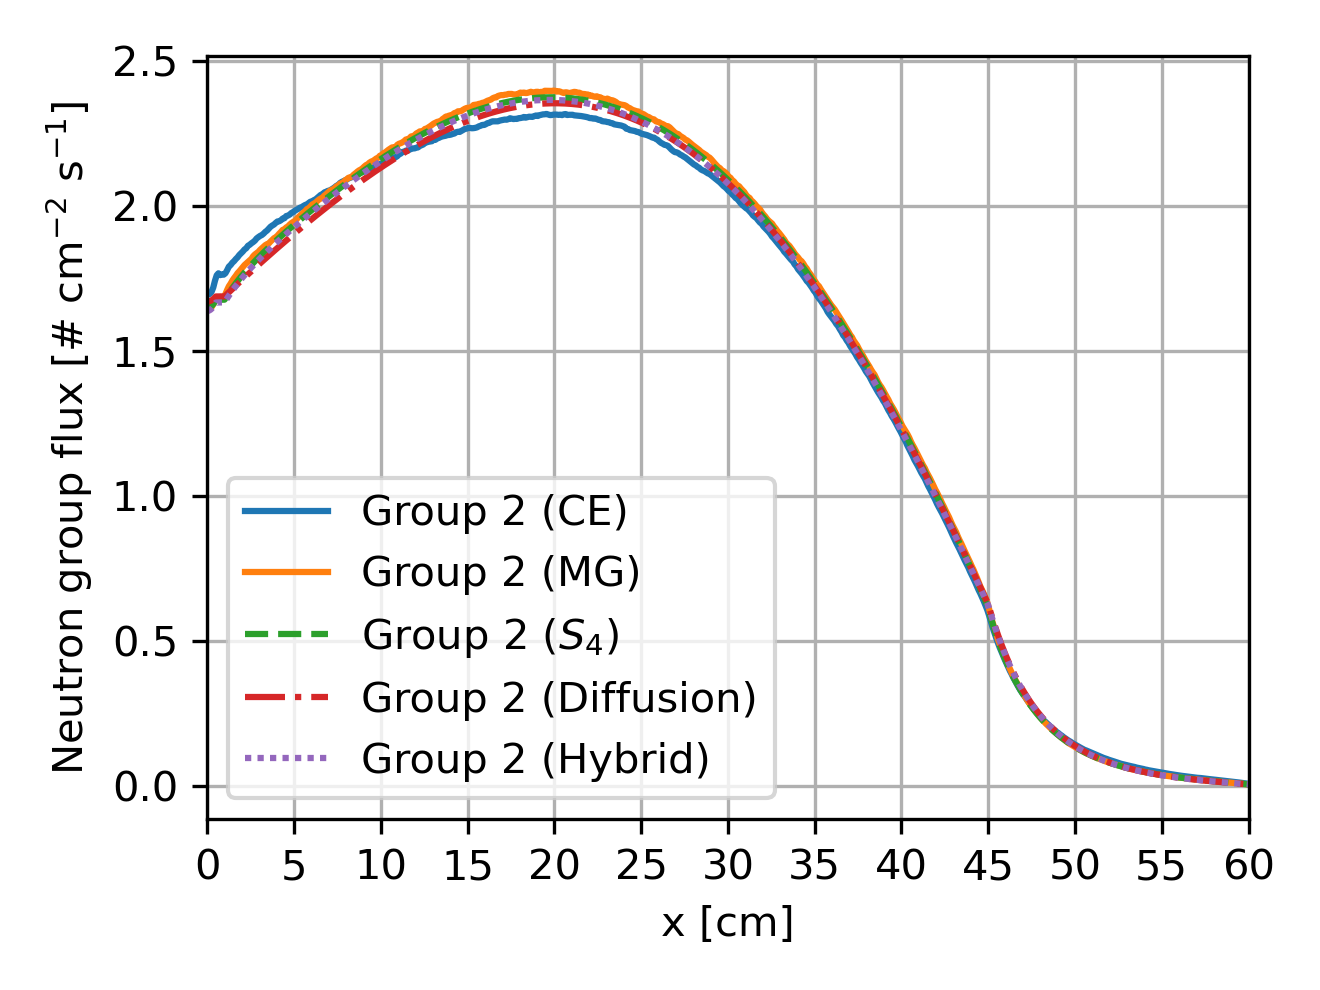
\includegraphics[width=\textwidth]{../images/case-3b-group-2-flux}
        \label{fig:c3bg2}
      \end{subfigure}
      \begin{subfigure}[t]{.45\textwidth}
        \centering
        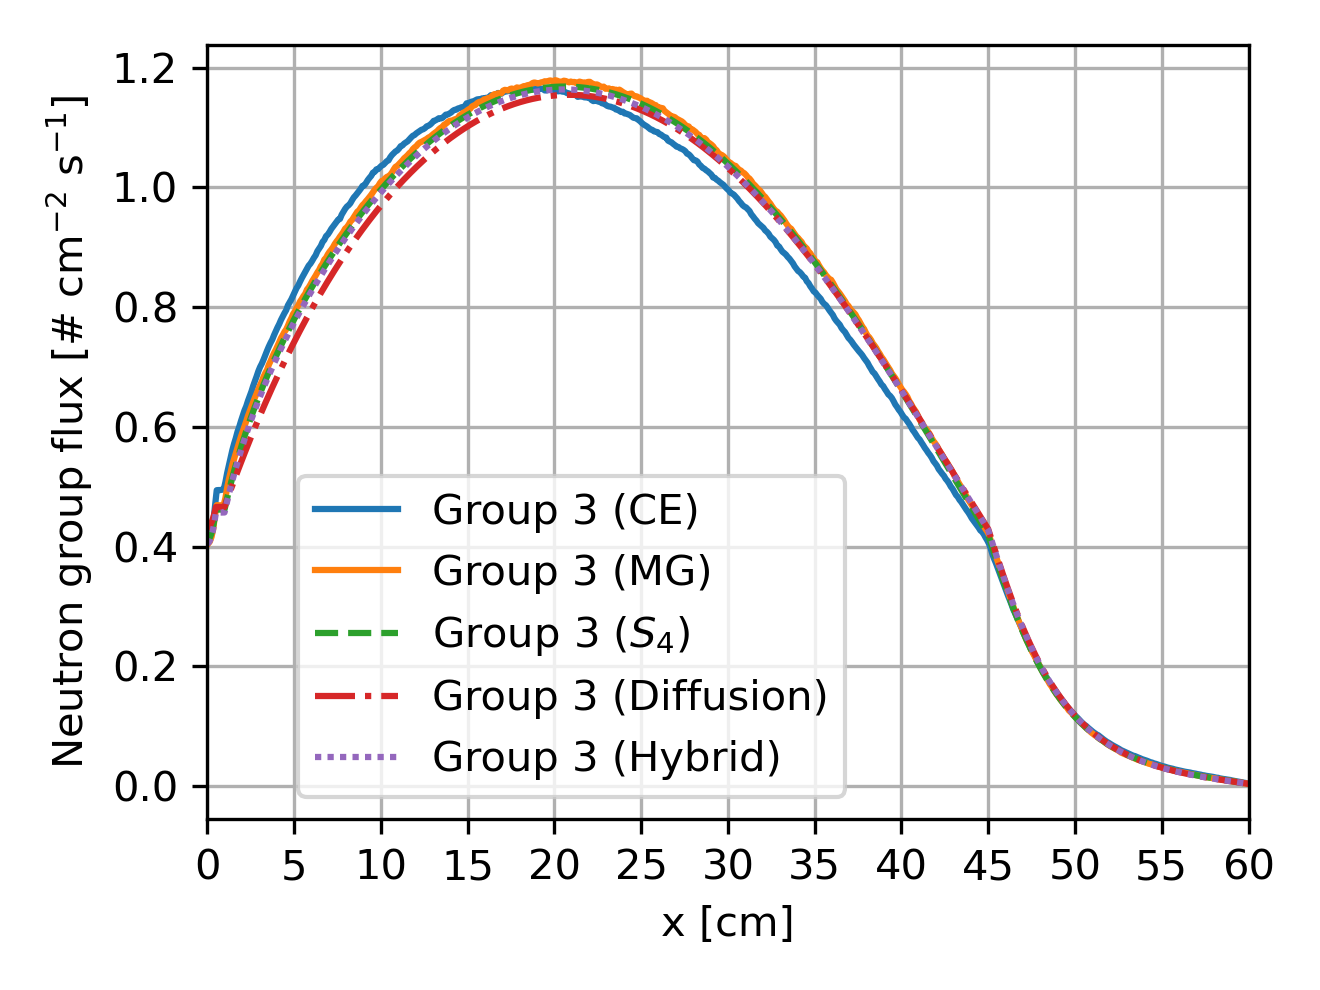
\includegraphics[width=\textwidth]{../images/case-3b-group-3-flux}
        \label{fig:c3bg3}
      \end{subfigure}
      \begin{subfigure}[t]{.45\textwidth}
        \centering
        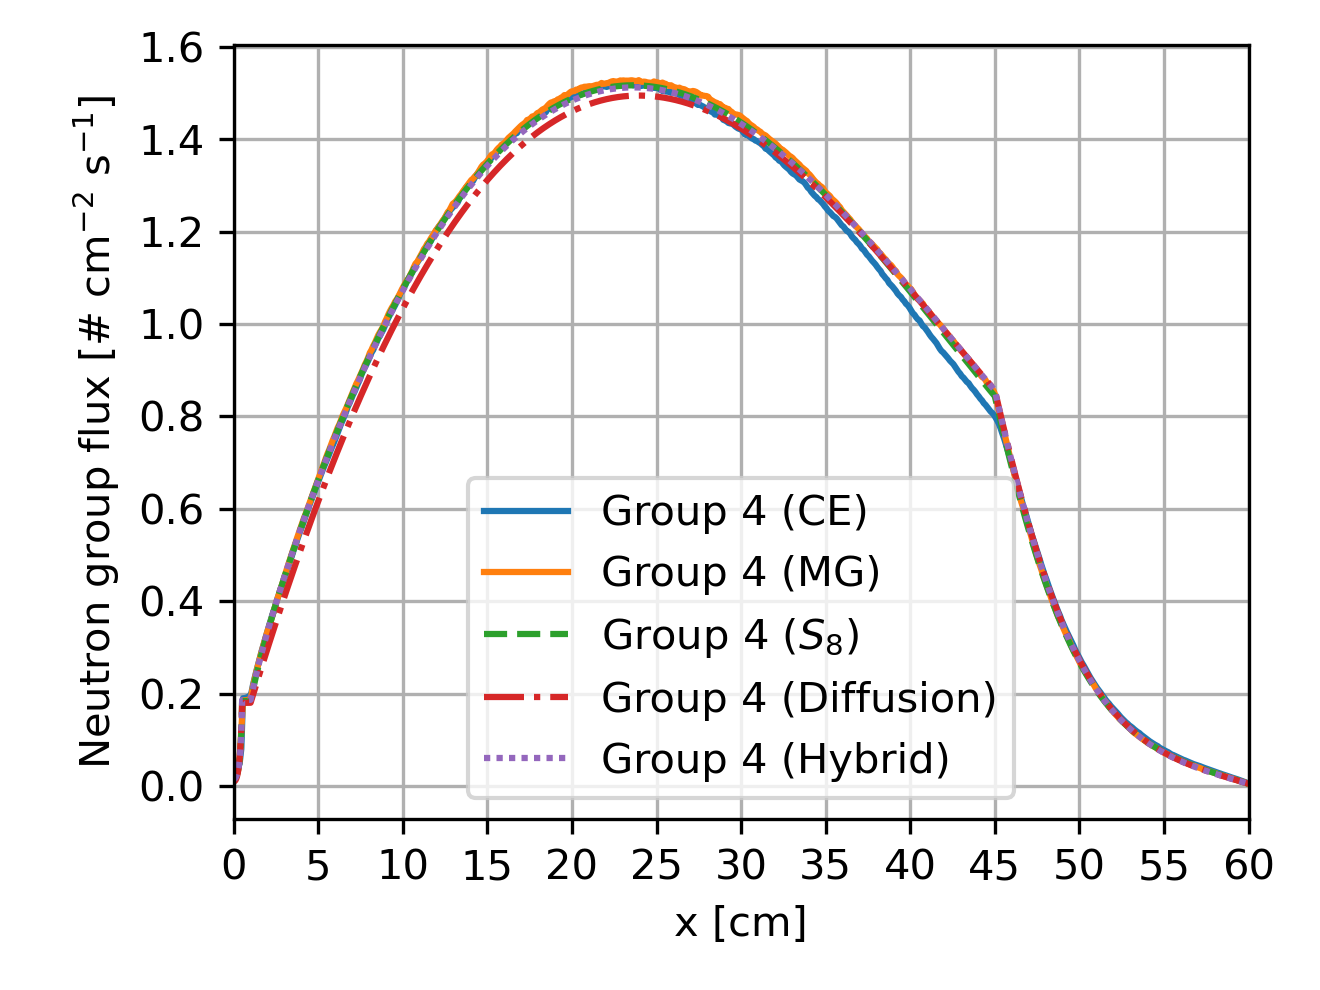
\includegraphics[width=\textwidth]{../images/case-3b-group-4-flux}
        \label{fig:c3bg4}
      \end{subfigure}
      \caption{Neutron group flux distributions for Case 3b.}
      \label{fig:c3bflux}
    \end{figure}
    \column{4cm}
    \begin{itemize}
      \item The OpenMC-CE (blue) and neutron diffusion (red) flux solutions deviate from the rest.
      \item Discrepancy with the OpenMC-CE solution is likely due to neutron energy group
        discretization
    \end{itemize}
  \end{columns}
\end{frame}

\begin{frame}
  \frametitle{Hybrid $S_N$-Diffusion Method: Preliminary Results}
  \begin{figure}
    \centering
    \begin{subfigure}[t]{.34\textwidth}
      \centering
      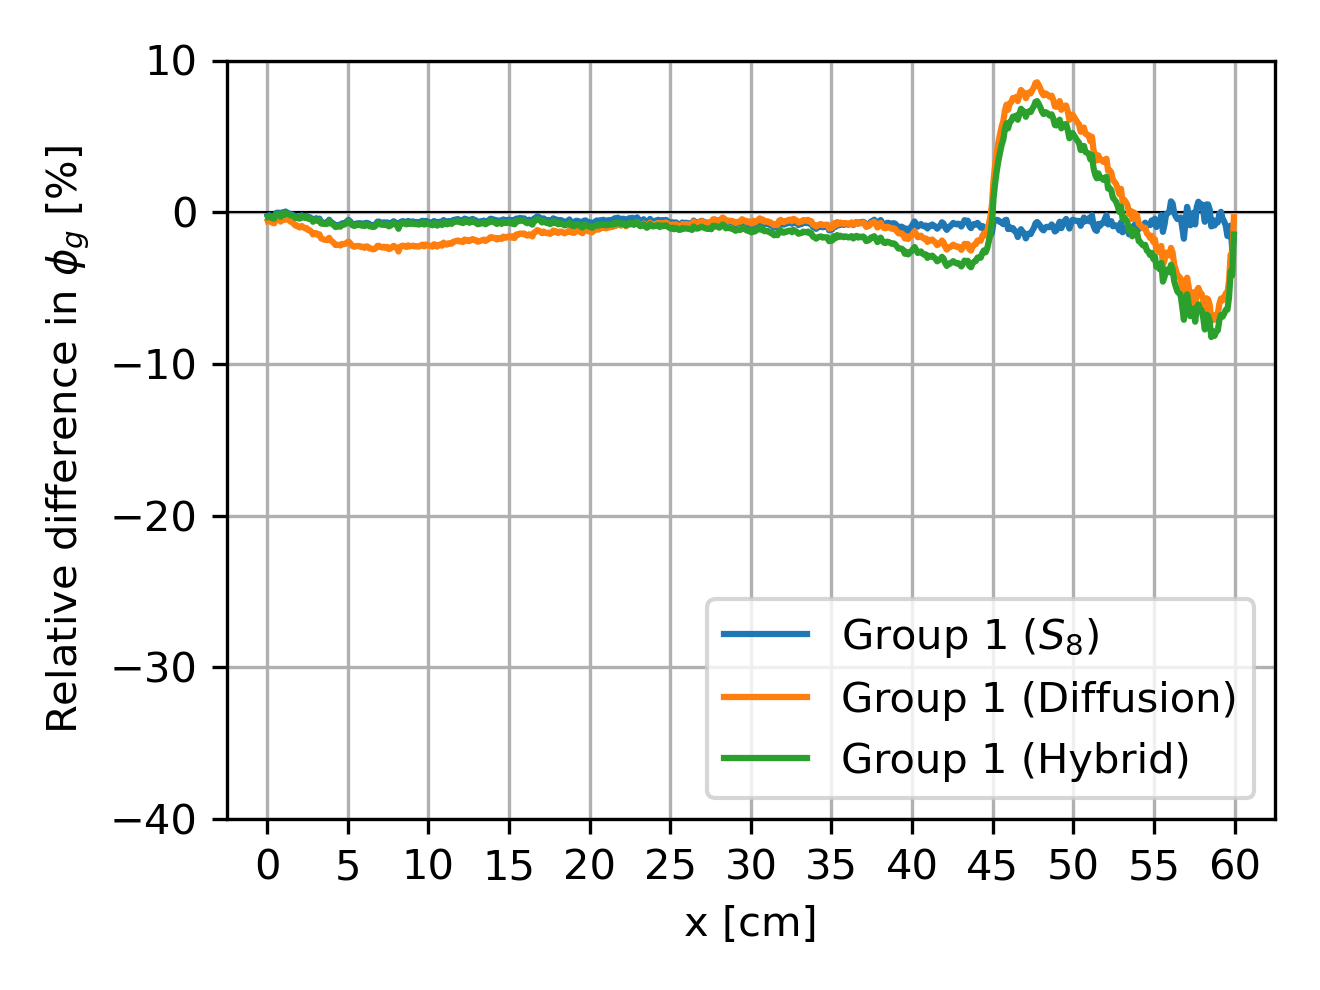
\includegraphics[width=\textwidth]{../images/case-3b-group-1-flux-error}
      \label{fig:c3bg1e}
    \end{subfigure}
    \begin{subfigure}[t]{.34\textwidth}
      \centering
      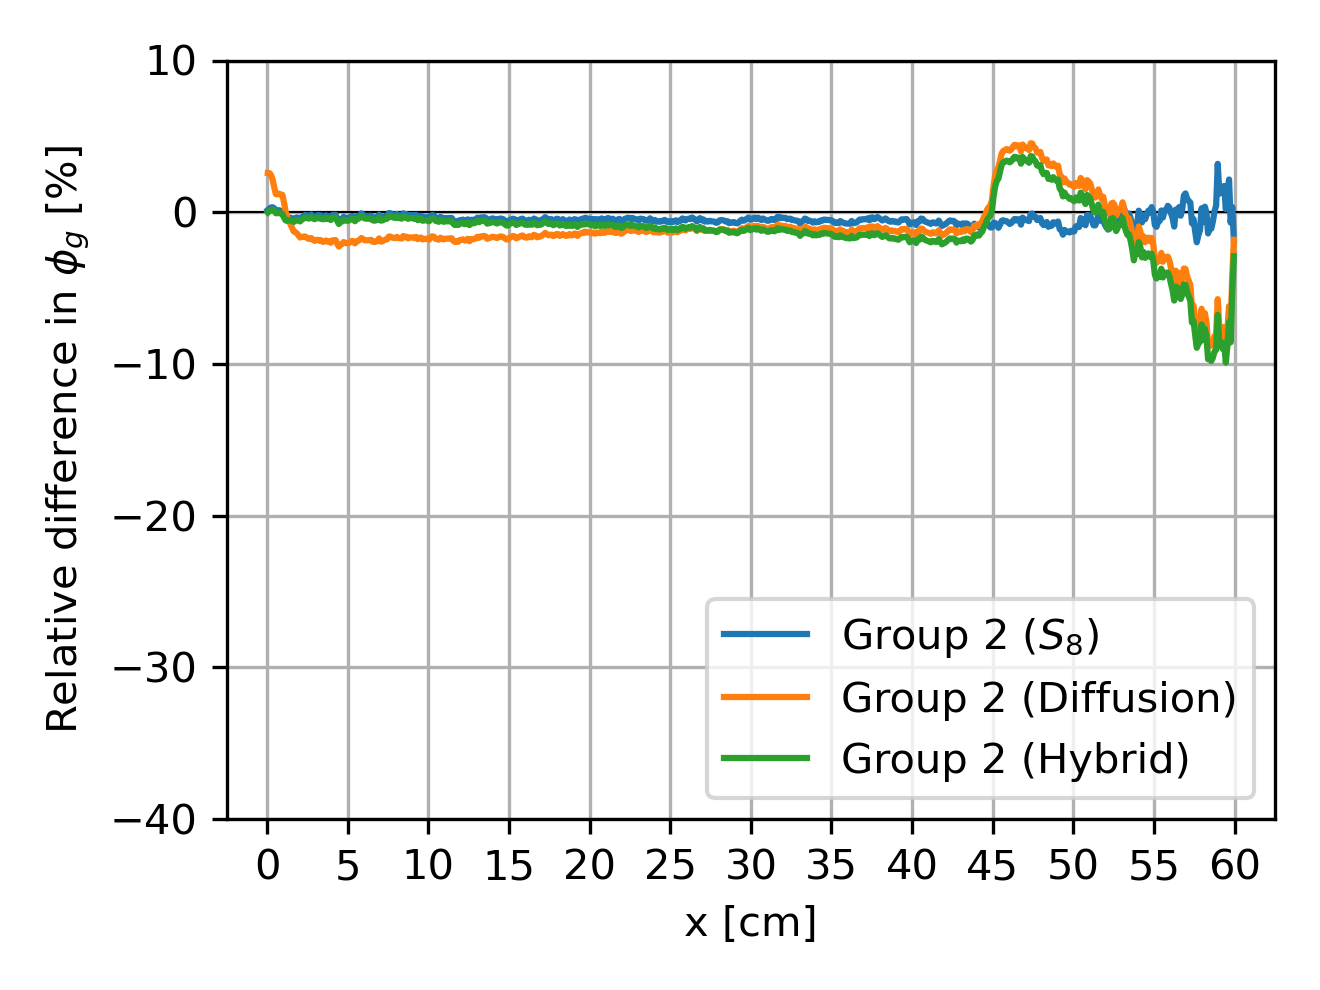
\includegraphics[width=\textwidth]{../images/case-3b-group-2-flux-error}
      \label{fig:c3bg2e}
    \end{subfigure}
    \begin{subfigure}[t]{.34\textwidth}
      \centering
      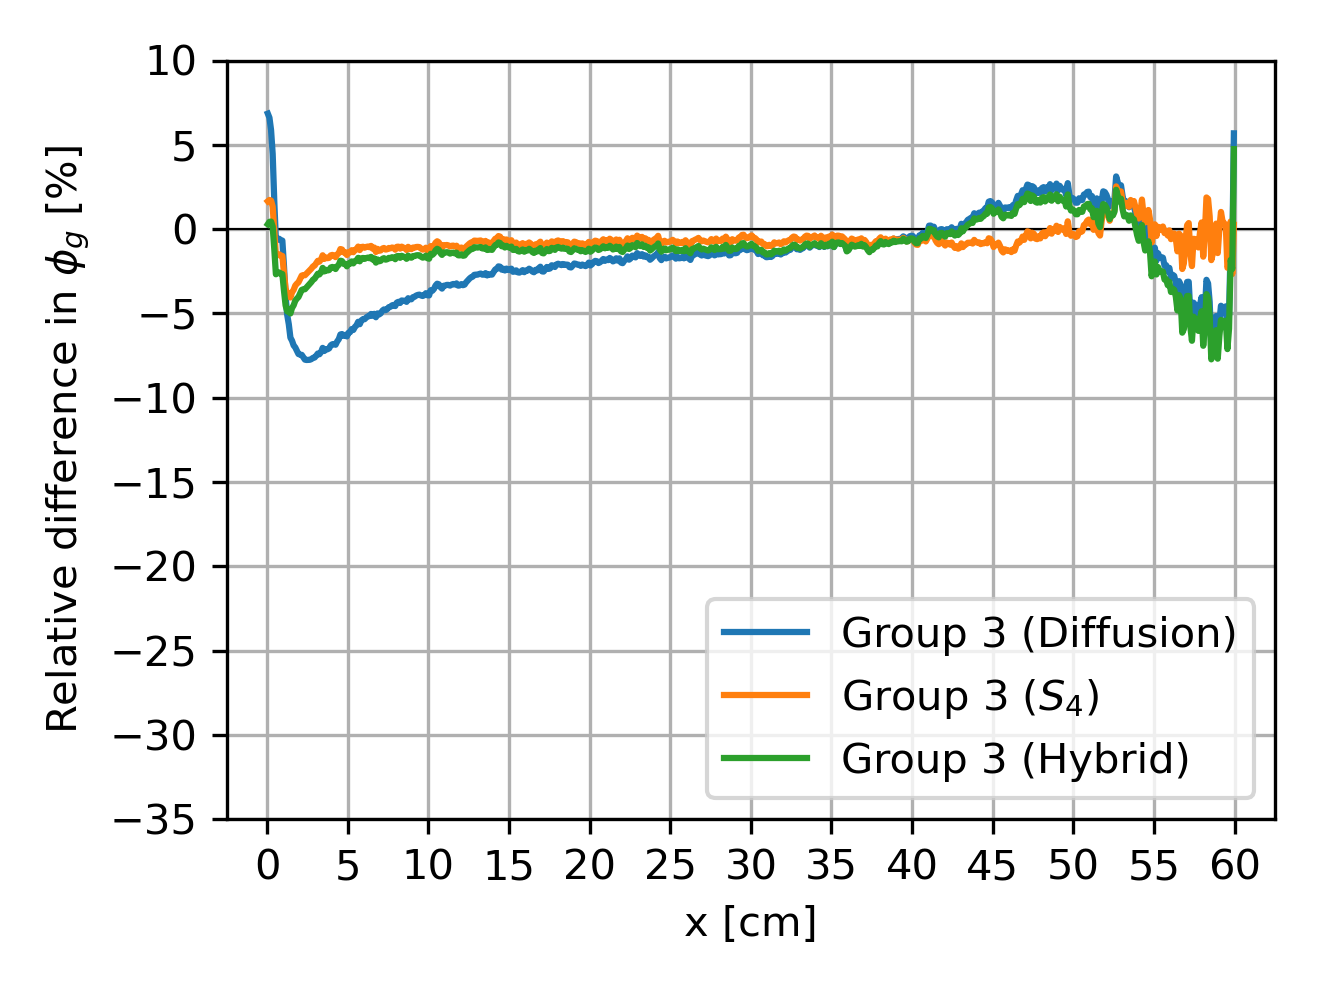
\includegraphics[width=\textwidth]{../images/case-3b-group-3-flux-error}
      \label{fig:c3bg3e}
    \end{subfigure}
    \begin{subfigure}[t]{.34\textwidth}
      \centering
      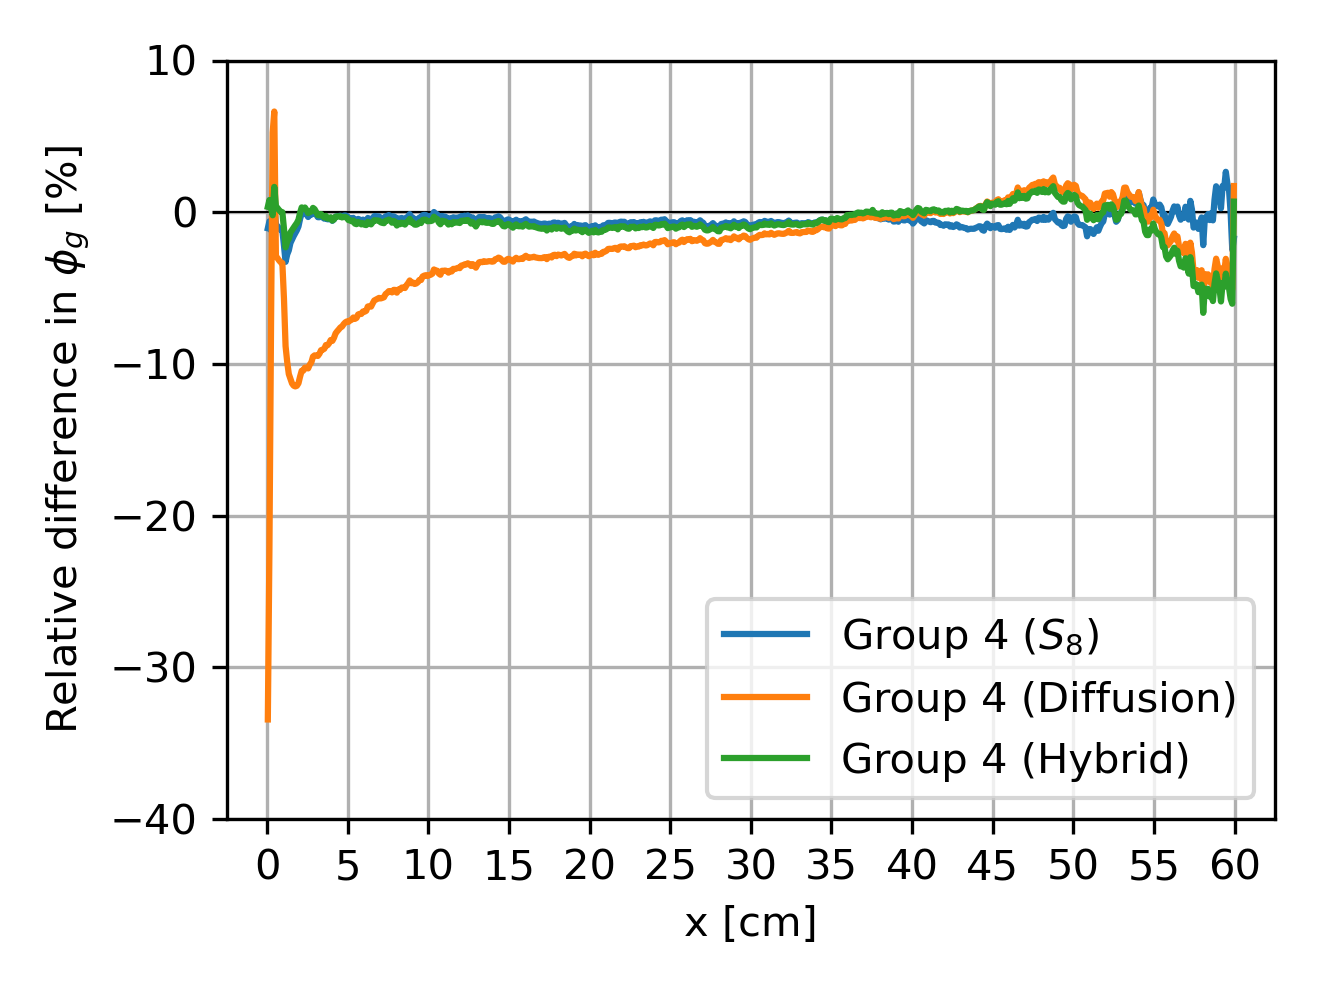
\includegraphics[width=\textwidth]{../images/case-3b-group-4-flux-error}
      \label{fig:c3bg4e}
    \end{subfigure}
    \caption{Relative differences of the neutron group flux distributions for Case 3b with respect
    to OpenMC-MG.}
    \label{fig:c3bfluxe}
  \end{figure}
\end{frame}

\begin{frame}
  \frametitle{Hybrid $S_N$-Diffusion Method: Preliminary Results}
  \begin{figure}[htb!]
    \centering
    \begin{subfigure}[t]{.35\textwidth}
      \centering
      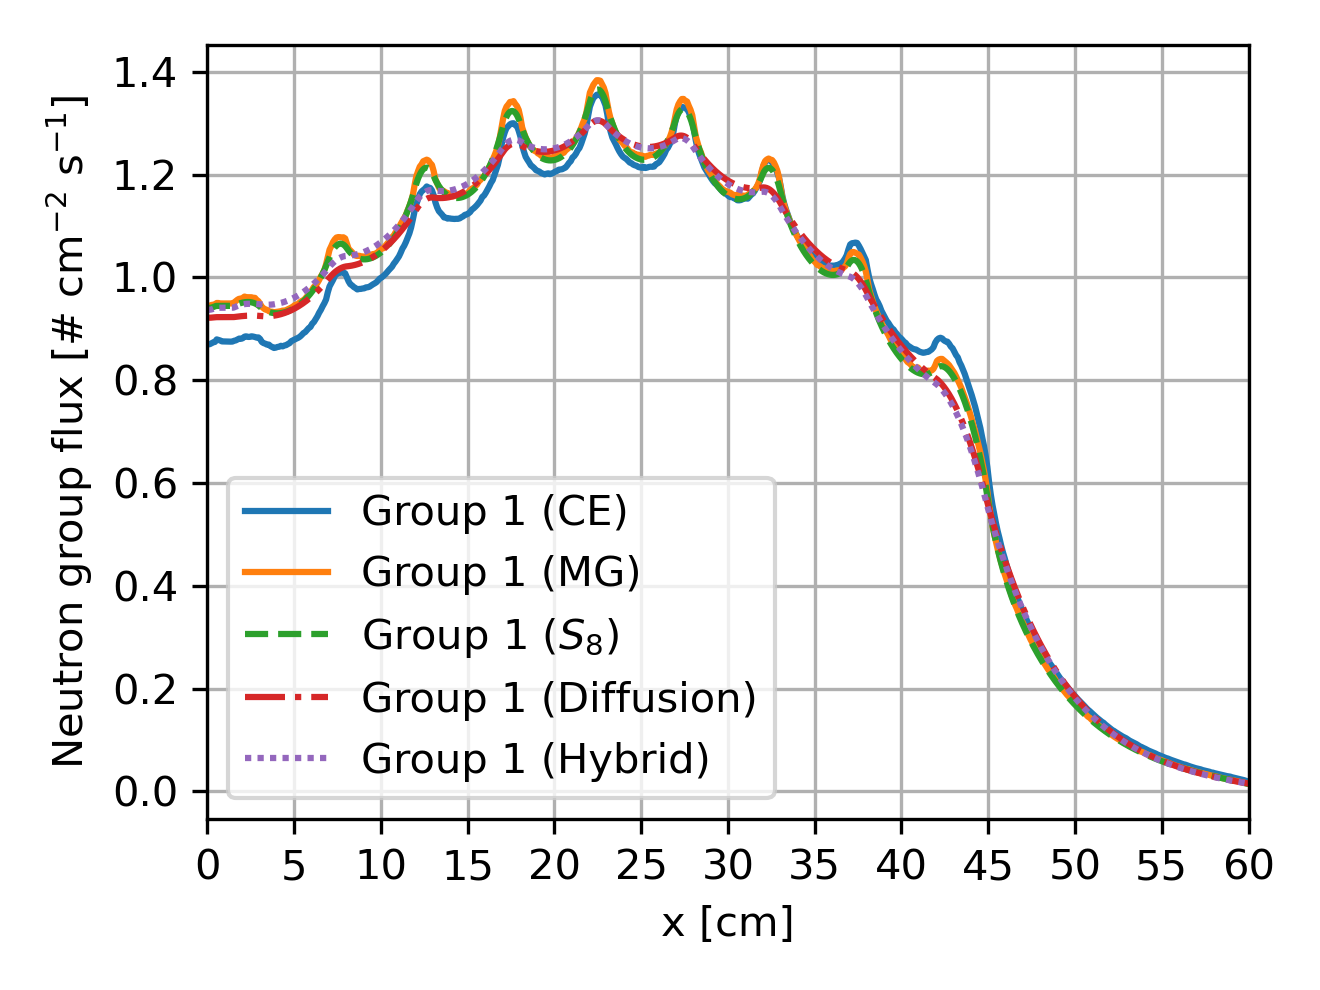
\includegraphics[width=\textwidth]{../images/case-5a-group-1-flux}
      \label{fig:c5ag1}
    \end{subfigure}
    \begin{subfigure}[t]{.35\textwidth}
      \centering
      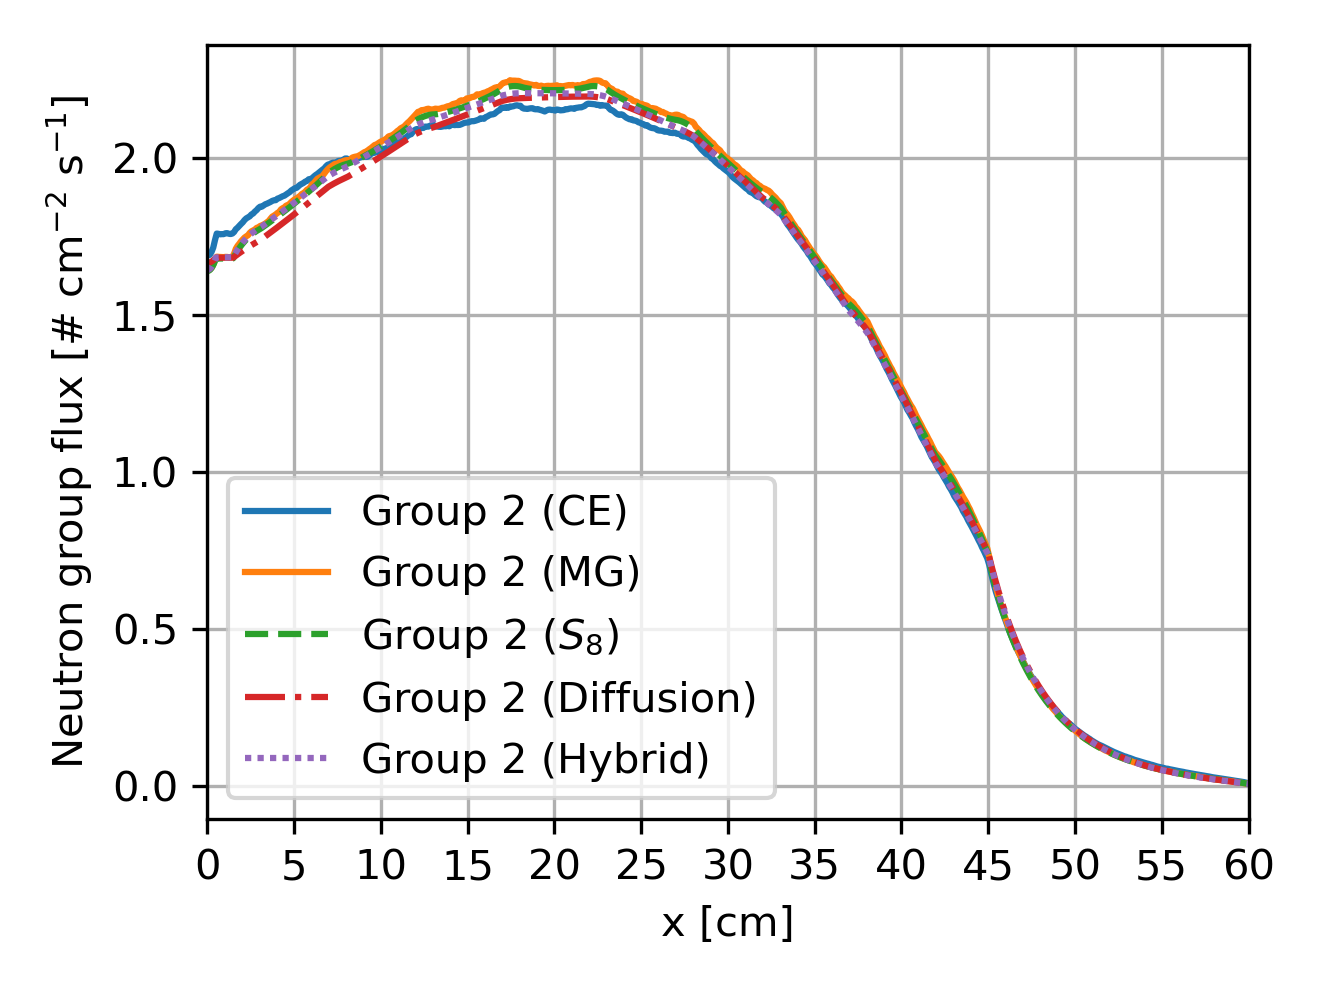
\includegraphics[width=\textwidth]{../images/case-5a-group-2-flux}
      \label{fig:c5ag2}
    \end{subfigure}
    \begin{subfigure}[t]{.35\textwidth}
      \centering
      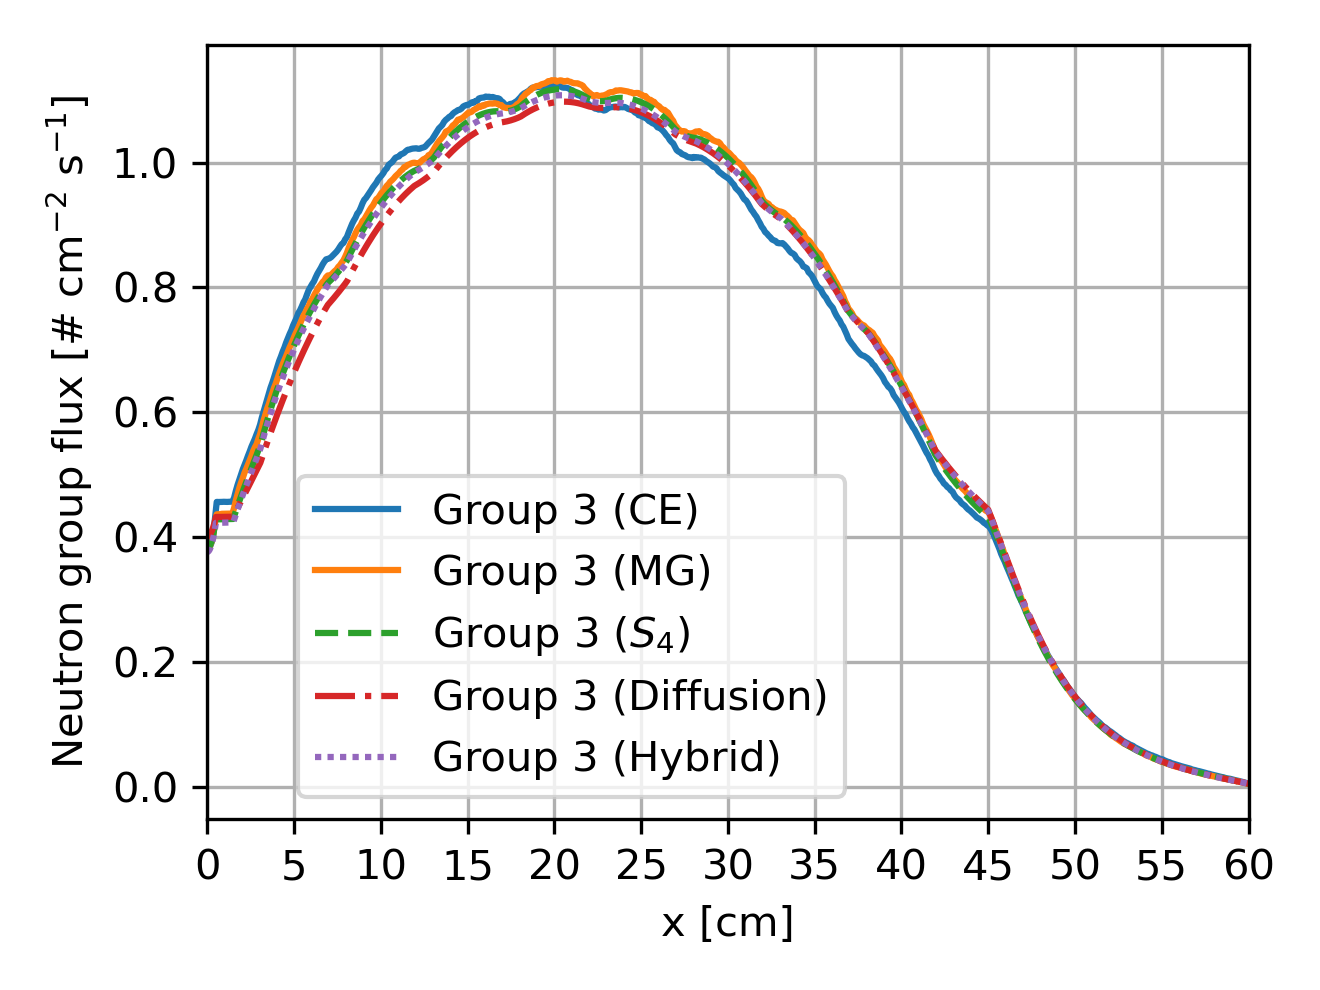
\includegraphics[width=\textwidth]{../images/case-5a-group-3-flux}
      \label{fig:c5ag3}
    \end{subfigure}
    \begin{subfigure}[t]{.35\textwidth}
      \centering
      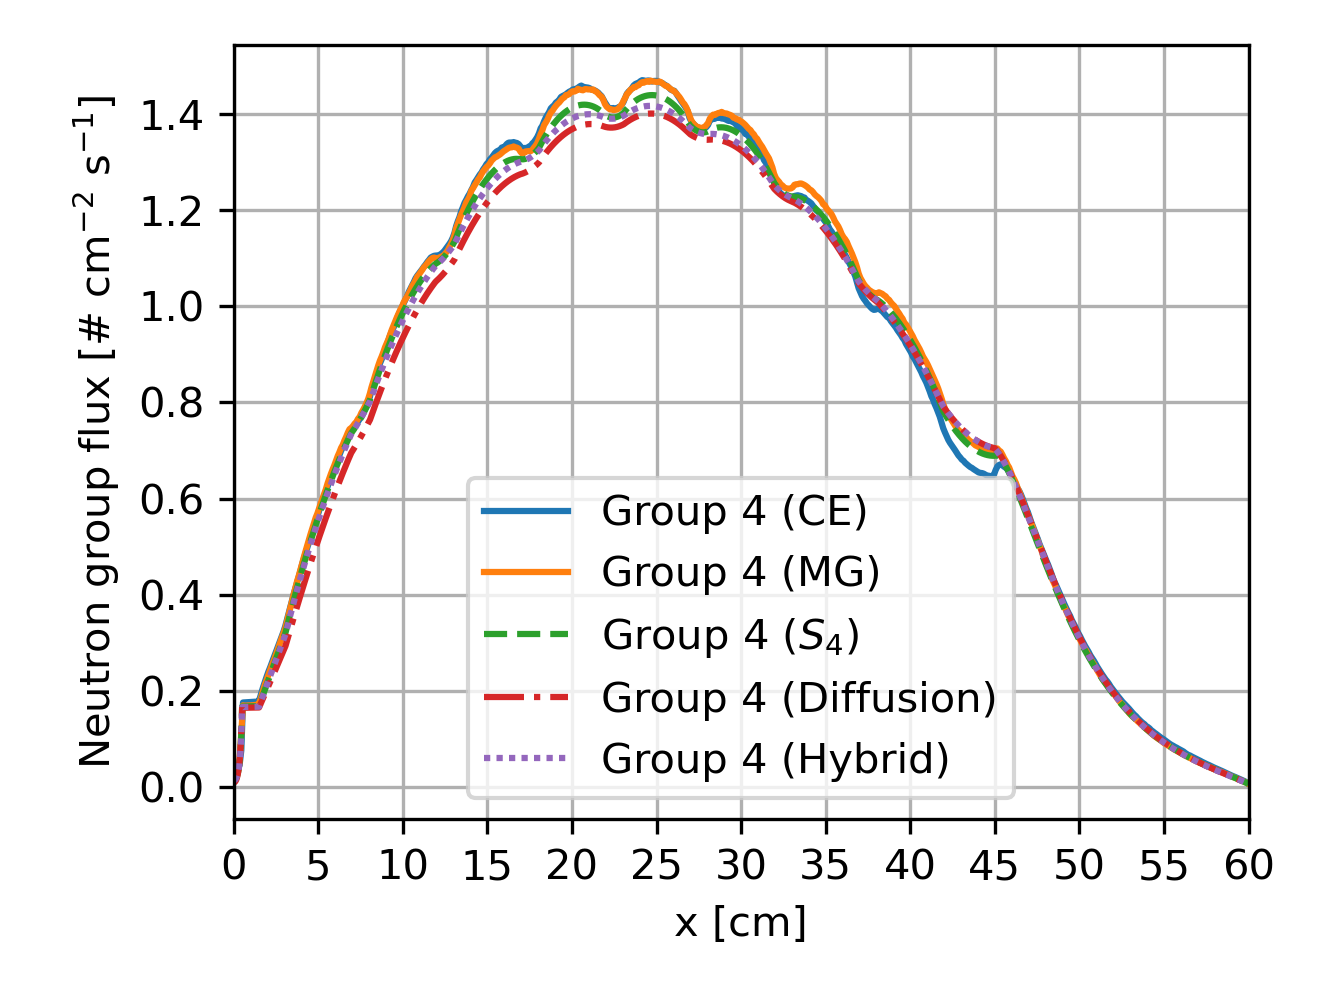
\includegraphics[width=\textwidth]{../images/case-5a-group-4-flux}
      \label{fig:c5ag4}
    \end{subfigure}
    \caption{Neutron group flux distributions for Case 5a.}
    \label{fig:c5aflux}
  \end{figure}
\end{frame}

\begin{frame}
  \frametitle{Hybrid $S_N$-Diffusion Method: Preliminary Results}
  \begin{figure}[htb!]
    \centering
    \begin{subfigure}[t]{.34\textwidth}
      \centering
      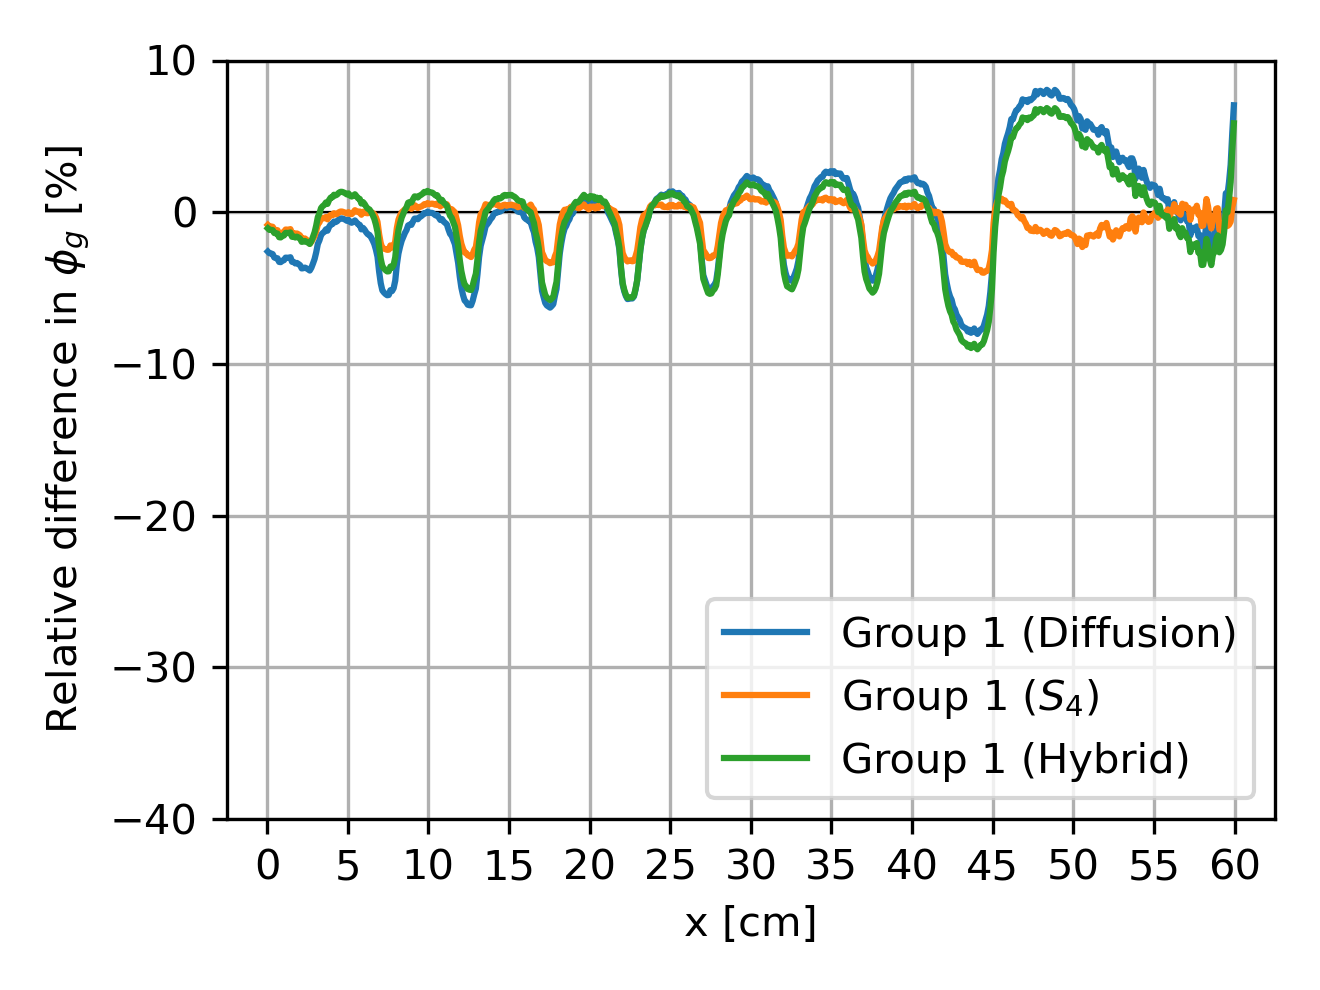
\includegraphics[width=\textwidth]{../images/case-5a-group-1-flux-error}
      \label{fig:c5ag1e}
    \end{subfigure}
    \begin{subfigure}[t]{.34\textwidth}
      \centering
      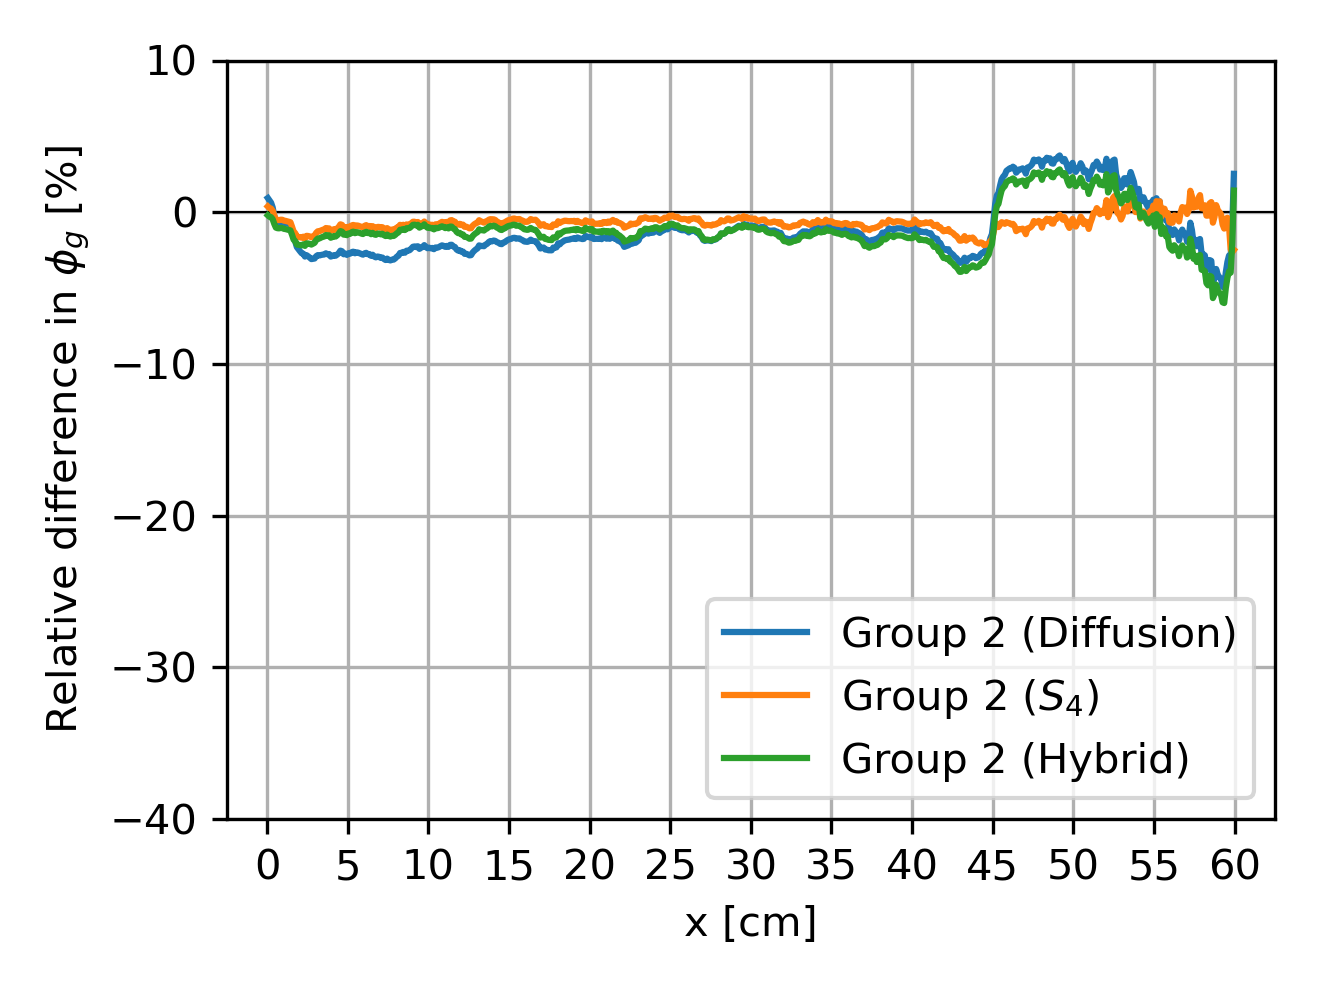
\includegraphics[width=\textwidth]{../images/case-5a-group-2-flux-error}
      \label{fig:c5ag2e}
    \end{subfigure}
    \begin{subfigure}[t]{.34\textwidth}
      \centering
      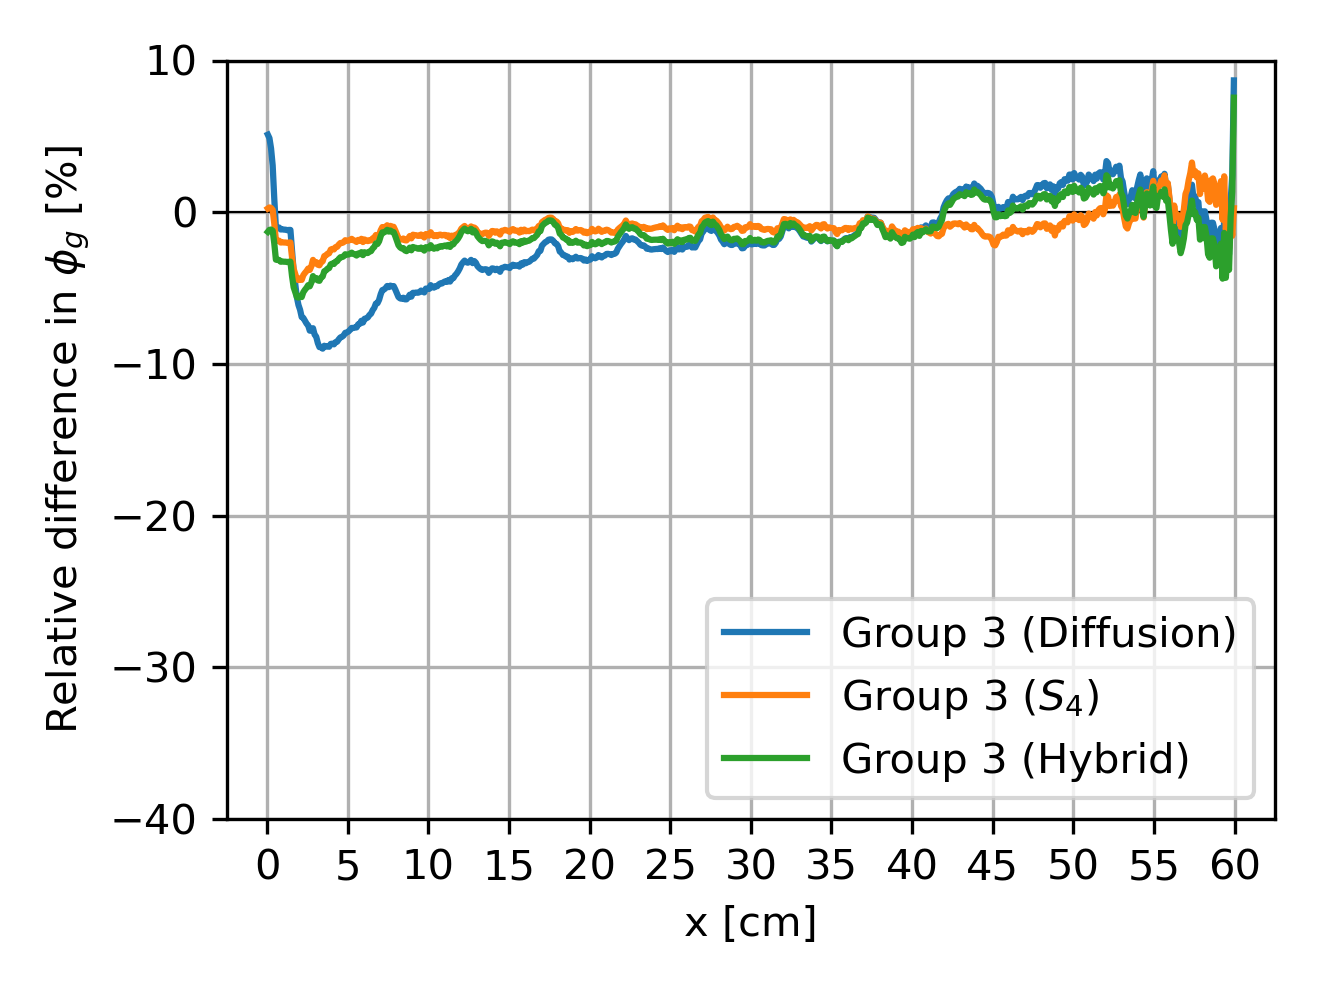
\includegraphics[width=\textwidth]{../images/case-5a-group-3-flux-error}
      \label{fig:c5ag3e}
    \end{subfigure}
    \begin{subfigure}[t]{.34\textwidth}
      \centering
      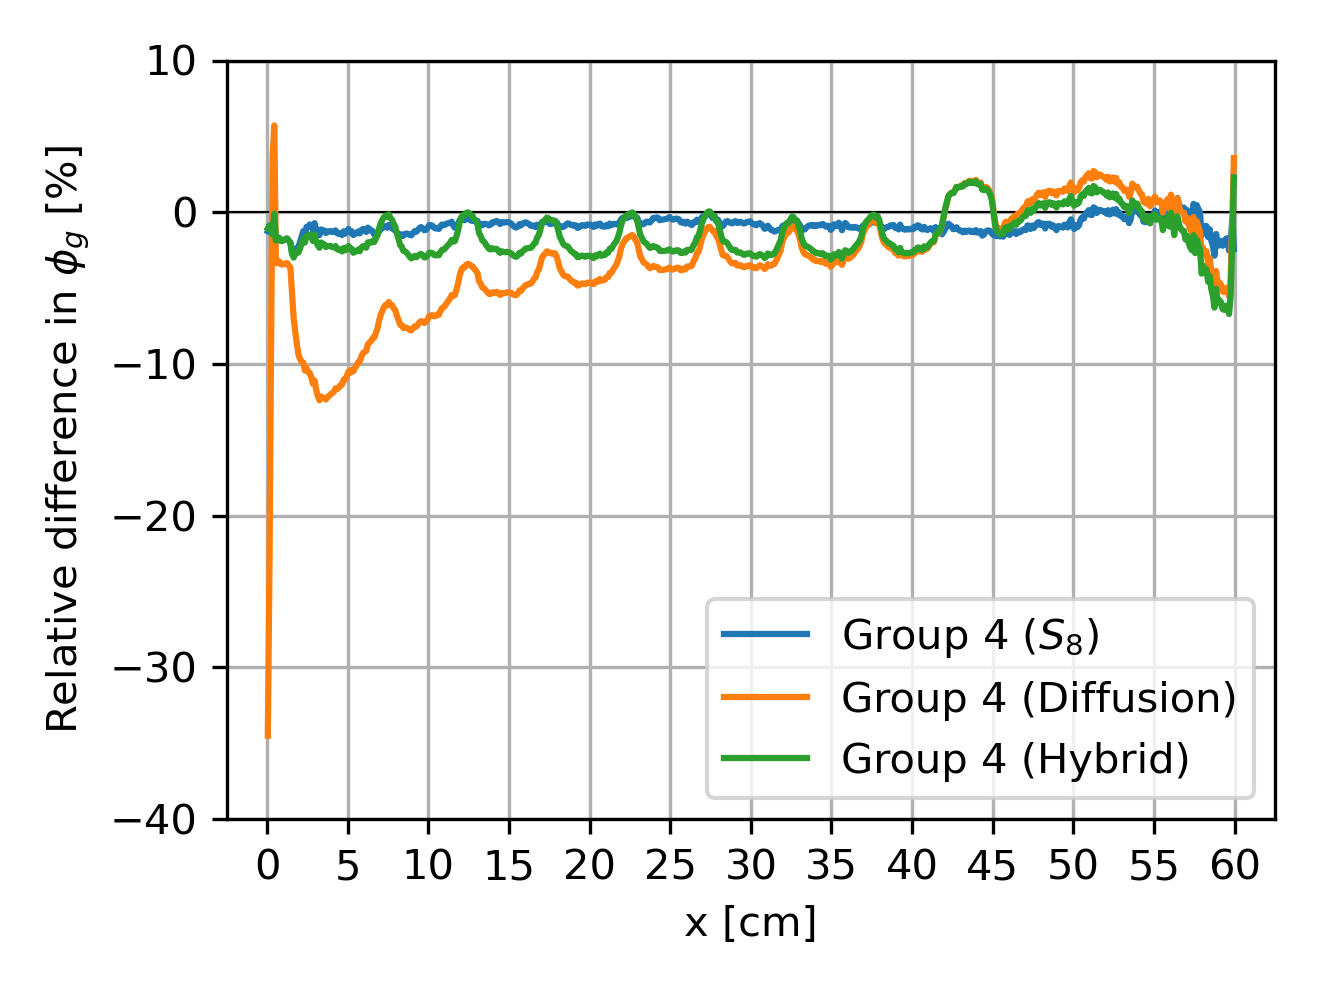
\includegraphics[width=\textwidth]{../images/case-5a-group-4-flux-error}
      \label{fig:c5ag4e}
    \end{subfigure}
    \caption{Relative differences of the neutron group flux distributions for Case 5a with respect
    to OpenMC-MG.}
    \label{fig:c5afluxe}
  \end{figure}
\end{frame}

\begin{frame}
  \frametitle{Hybrid $S_N$-Diffusion Method: Preliminary Results}
  \begin{table}
    \centering
    \footnotesize
    \caption{Normalized flux error $\varepsilon$ for Case 3b with respect to OpenMC-MG.}
    \begin{tabular}{c S S S S}
      \toprule
      {\multirow{2}{*}{\textbf{Method}}} &
      \multicolumn{4}{c}{\textbf{Normalized flux error,} $\bm{\varepsilon_g}$} \\
      \cmidrule{2-5}
      & {\textbf{Group 1}} & {\textbf{Group 2}} & {\textbf{Group 3}} &
      {\textbf{Group 4}} \\
      \midrule
      $S_8$     & 0.0066 & 0.0048 & 0.0058 & 0.0067 \\
      Diffusion & 0.0144 & 0.0147 & 0.0258 & 0.0267 \\
      Hybrid    & 0.0122 & 0.0099 & 0.0087 & 0.0084 \\
      \bottomrule
    \end{tabular}
    \label{table:c3berror}
  \end{table}
  \begin{table}
    \centering
    \footnotesize
    \caption{Normalized flux error $\varepsilon$ for Case 5a with respect to OpenMC-MG.}
    \begin{tabular}{c S S S S}
      \toprule
      {\multirow{2}{*}{\textbf{Method}}} &
      \multicolumn{4}{c}{\textbf{Normalized flux error,} $\bm{\varepsilon_g}$} \\
      \cmidrule{2-5}
      & {\textbf{Group 1}} & {\textbf{Group 2}} & {\textbf{Group 3}} &
      {\textbf{Group 4}} \\
      \midrule
      $S_8$     & 0.0078 & 0.0074 & 0.0083 & 0.0085 \\
      Diffusion & 0.0305 & 0.0202 & 0.0313 & 0.0406 \\
      Hybrid    & 0.0290 & 0.0147 & 0.0143 & 0.0216 \\
      \bottomrule
    \end{tabular}
    \label{table:c5aerror}
  \end{table}
\end{frame}

\begin{frame}
  \frametitle{Hybrid $S_N$-Diffusion Method: Preliminary Results}
  \begin{figure}
    \centering
    \begin{subfigure}[t]{.35\textwidth}
      \centering
      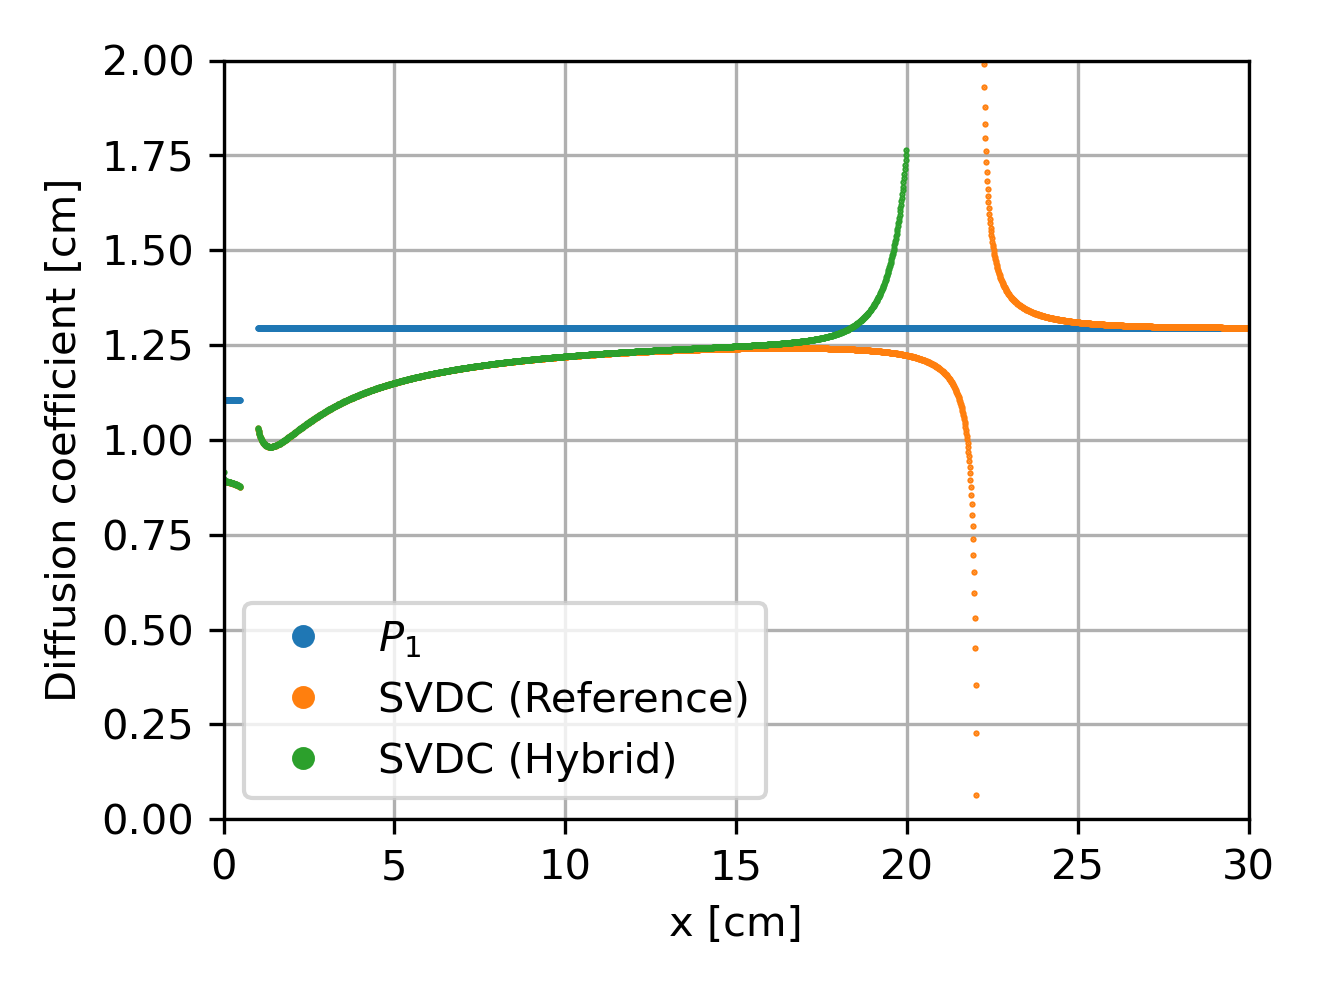
\includegraphics[width=\textwidth]{../images/case-3b-group-1-diffcoef}
      \label{fig:c3bg1dc}
    \end{subfigure}
    \begin{subfigure}[t]{.35\textwidth}
      \centering
      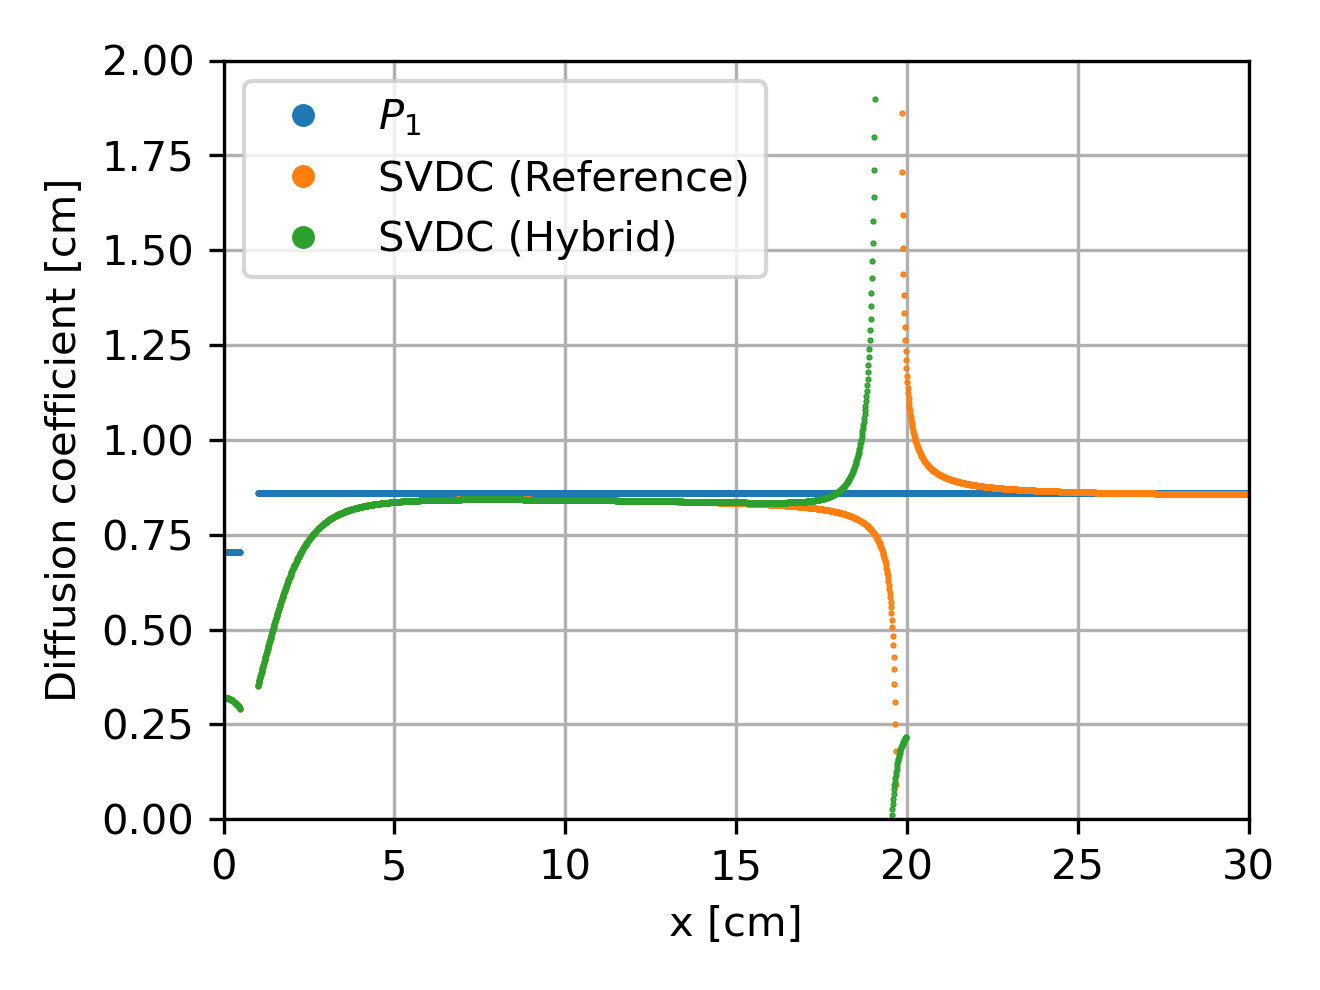
\includegraphics[width=\textwidth]{../images/case-3b-group-2-diffcoef}
      \label{fig:c3bg2dc}
    \end{subfigure}
    \begin{subfigure}[t]{.35\textwidth}
      \centering
      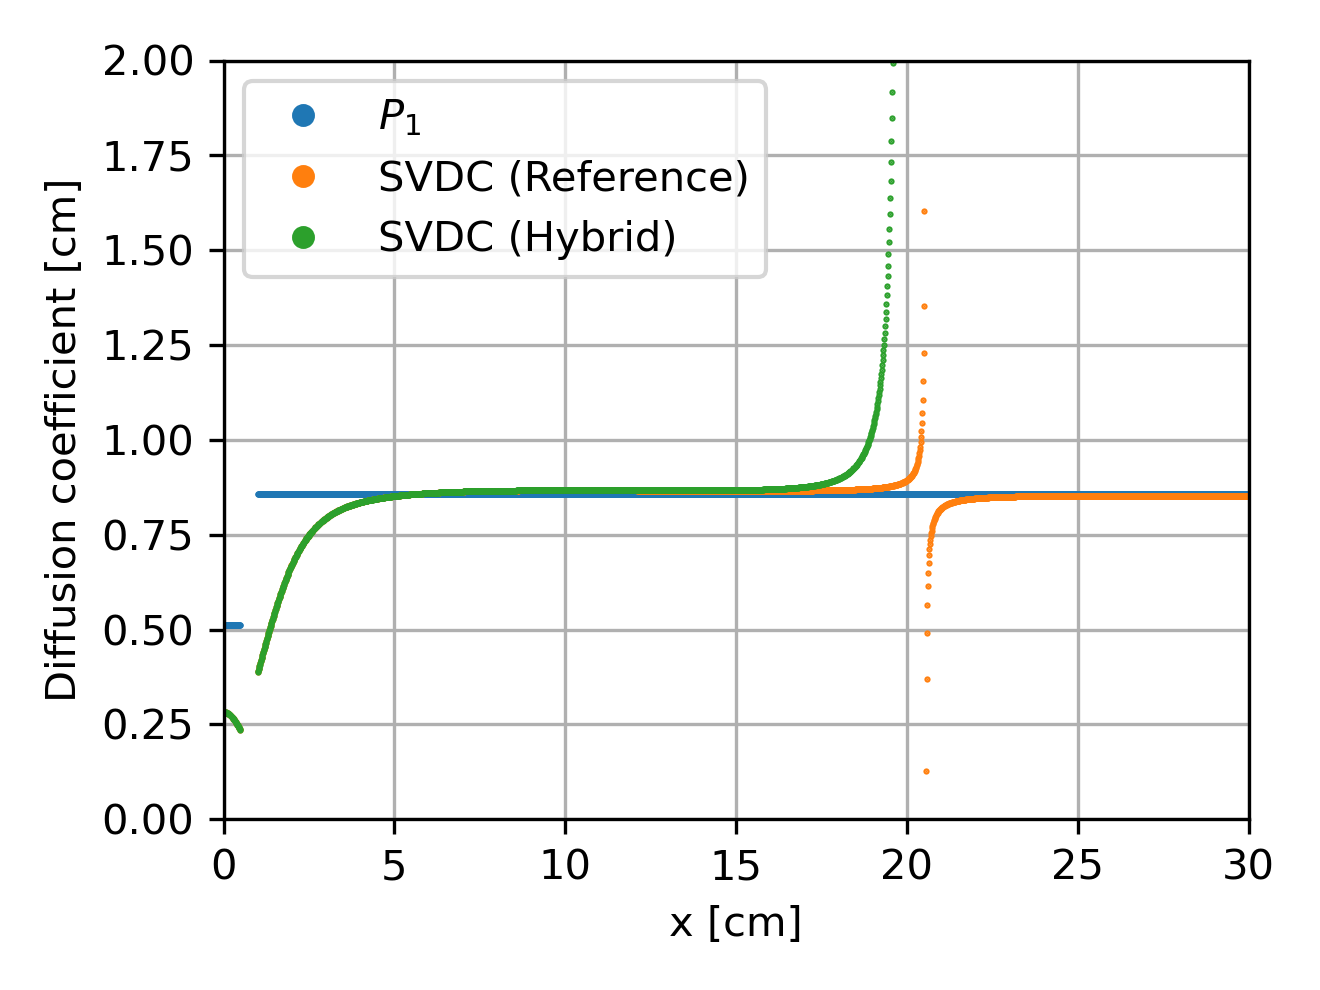
\includegraphics[width=\textwidth]{../images/case-3b-group-3-diffcoef}
      \label{fig:c3bg3dc}
    \end{subfigure}
    \begin{subfigure}[t]{.35\textwidth}
      \centering
      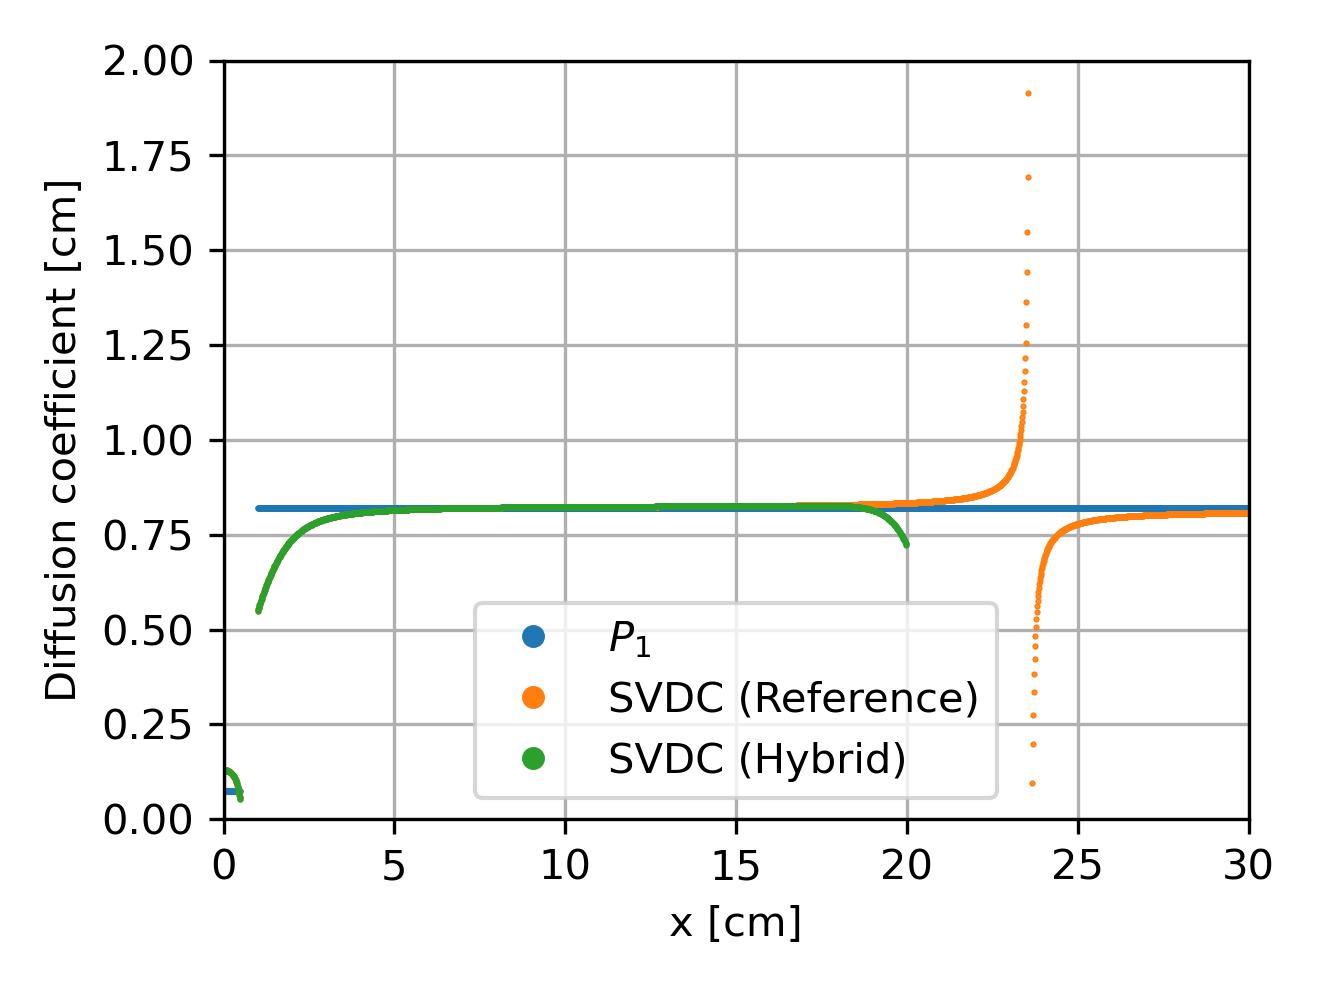
\includegraphics[width=\textwidth]{../images/case-3b-group-4-diffcoef}
      \label{fig:c3bg4dc}
    \end{subfigure}
    \caption{Diffusion coefficients for Case 3b between $x=0$ cm and $x=30$ cm.}
    \label{fig:c3bdiffcoef}
  \end{figure}
\end{frame}

\begin{frame}
  \frametitle{Hybrid $S_N$-Diffusion Method: Preliminary Results}
  \begin{figure}
    \centering
    \begin{subfigure}[t]{.35\textwidth}
      \centering
      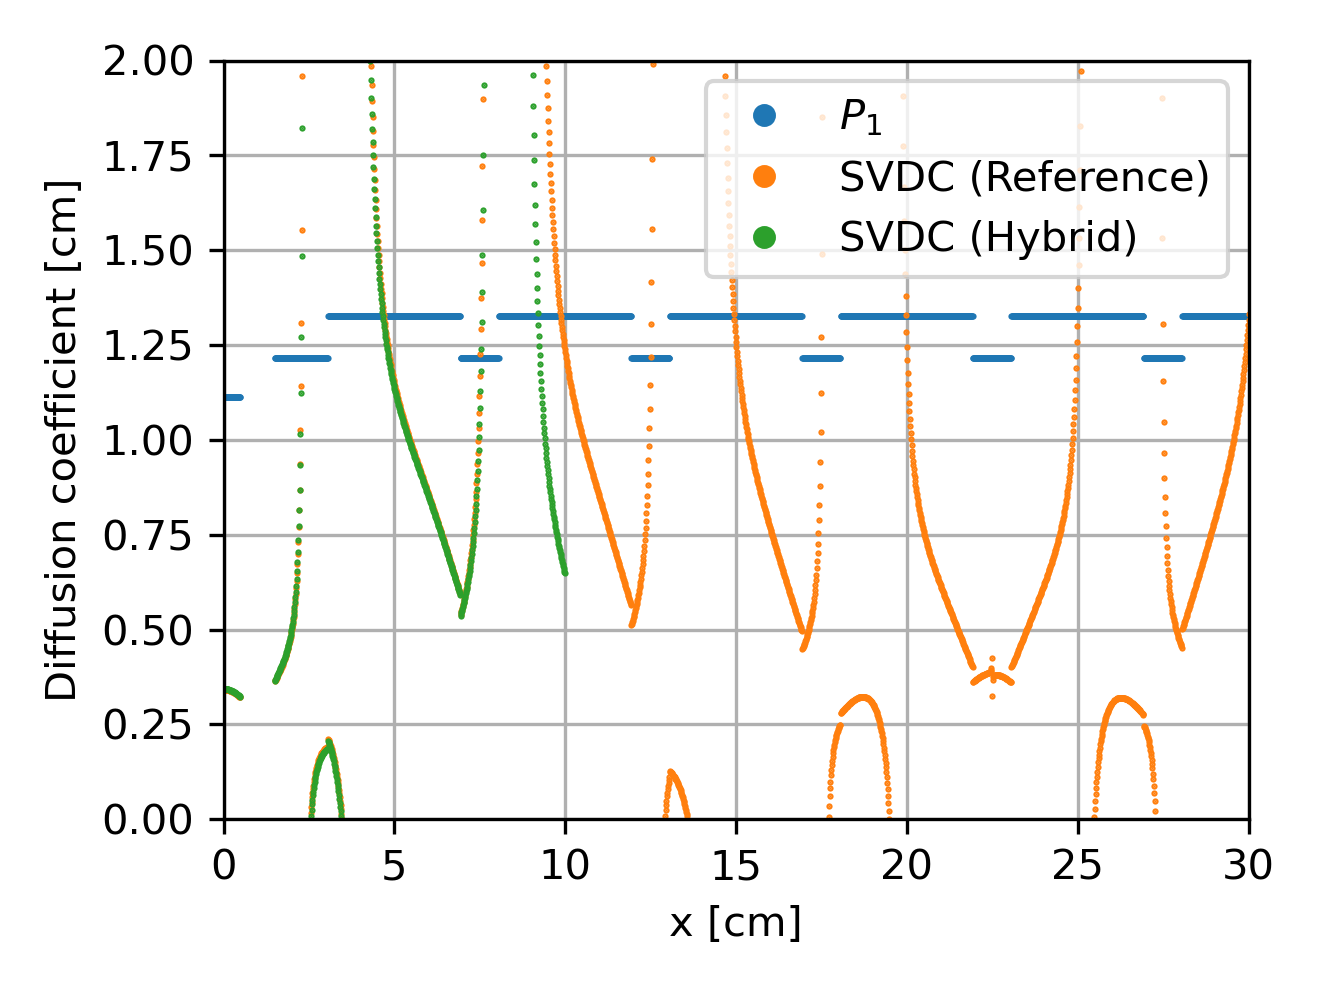
\includegraphics[width=\textwidth]{../images/case-5a-group-1-diffcoef}
      \label{fig:c5ag1dc}
    \end{subfigure}
    \begin{subfigure}[t]{.35\textwidth}
      \centering
      \includegraphics[width=\textwidth]{../images/case-5a-group-2-diffcoef}
      \label{fig:c5ag2dc}
    \end{subfigure}
    \begin{subfigure}[t]{.35\textwidth}
      \centering
      \includegraphics[width=\textwidth]{../images/case-5a-group-3-diffcoef}
      \label{fig:c5ag3dc}
    \end{subfigure}
    \begin{subfigure}[t]{.35\textwidth}
      \centering
      \includegraphics[width=\textwidth]{../images/case-5a-group-4-diffcoef}
      \label{fig:c5ag4dc}
    \end{subfigure}
    \caption{Diffusion coefficients for Case 5a between $x=0$ cm and $x=30$ cm.}
    \label{fig:c5adiffcoef}
  \end{figure}
\end{frame}

\begin{frame}
  \frametitle{Hybrid $S_N$-Diffusion Method: Preliminary Results}
  \begin{block}{\textbf{Summary}}
    \begin{itemize}
      \item The hybrid $S_N$-Diffusion method improves the multiplication factor and neutron flux
        estimates from the neutron diffusion method by introducing transport corrections from the
        $S_N$ method.
      \item The $S_N$ subsolver runs on a smaller subdomain around the control rod to reduce
        computational costs.
      \item In the $S_N$ subsolver, the SVDCs converge faster than the neutron flux.
      \item Additional work is required on:
        \begin{itemize}
          \item how to handle infinite diffusion coefficient values wherever the flux gradient
            approaches zero
          \item determining correction region and buffer zone sizes with minimal preprocessing work
        \end{itemize}
    \end{itemize}
  \end{block}
\end{frame}

\subsection{Proposed Work}
\begin{frame}
  \frametitle{Hybrid $S_N$-Diffusion Method: Proposed Work}
  \begin{block}{\textbf{Development of a Hybrid $S_N$-Diffusion Method for Control Rod Modeling}}
    \textbf{Sub-objectives}
    \begin{enumerate}
      \item Development \& Implementation of the Hybrid Method in Moltres
      \item Verification of the Hybrid Method Against Reference OpenMC Calculations
      \item Computational Performance Characterization of the Hybrid Method
    \end{enumerate}
  \end{block}
\end{frame}

\begin{frame}
  \frametitle{Hybrid $S_N$-Diffusion Method: Proposed Work}
  \textbf{Sub-objective 1: Development \& Implementation of the Hybrid Method in Moltres}
  \vspace{.2cm}

  \textbf{Implementation Details:}
  \begin{itemize}
    \item 3-D $S_N$ solver with a diffusion synthetic acceleration scheme
    \item Automate multigroup $S_N$-diffusion coupling through the MOOSE MultiApp and Action
      systems
    \item Supporting features (e.g., SVDC calculations, buffer zone calculations)
  \end{itemize}
\end{frame}

\begin{frame}
  \frametitle{Hybrid $S_N$-Diffusion Method: Proposed Work}
  \textbf{Sub-objective 1: Development \& Implementation of the Hybrid Method in Moltres}
  \vspace{.2cm}

  \textbf{\gls{SVDC} Calculation}

  The existing formulation for SVDCs are undefined at flux peaks and troughs:
  \begin{align}
    D^s_g(x) &= -J^{tr}_g(x)\bigg/\frac{d\phi^{tr}_g(x)}{dx} \nonumber
  \end{align}
  I will explore alternative formulations to avoid division by the flux gradient. For instance,
  Tomatis \& Dall'Osso \cite{tomatis_application_2011} developed the following formulation for
  additive corrections for the Ronen method:
  \begin{align}
    \delta D(x_{i+1/2},E) =& -\delta J(x_{i+1/2},E) \frac{(\Delta x_{i+1}+\Delta x_i)/2}{
    \phi(x_{i+1},E)+\phi(x_i,E)}
    \shortintertext{where}
    x_i =& \mbox{ $i$-th spatial interval,} \nonumber \\
    \delta J(x,E) =& J_{tr}(x,E) - J_D(x,E), \nonumber \\
    \Delta x_i =& \mbox{ size of $i$-th spatial interval.} \nonumber
  \end{align}
\end{frame}

\begin{frame}
  \frametitle{Hybrid $S_N$-Diffusion Method: Proposed Work}
  \textbf{Sub-objective 1: Development \& Implementation of the Hybrid Method in Moltres}
  \vspace{.2cm}
  
  \textbf{Correction Region Size}
  \vspace{.1cm}

  The correction region represents the problem domain of the $S_N$ sub-solver.
  \vspace{.2cm}
  
  I will investigate 2-D and 3-D problems derived from the MSRE design to create a set of criteria
  for the minimum required correction region size. My preliminary work showed that the:
  \begin{itemize}
    \item geometrical heterogeneity and
    \item optical thickness
  \end{itemize}
  strongly influence the \gls{SVDC} and the minimum correction region size.
\end{frame}

\begin{frame}
  \frametitle{Hybrid $S_N$-Diffusion Method: Proposed Work}
  \textbf{Sub-objective 1: Development \& Implementation the Hybrid Method in Moltres}
  \vspace{.2cm}

  \textbf{Autonomous Buffer Zone Determination}
  
\end{frame}

\begin{frame}
  \frametitle{Hybrid $S_N$-Diffusion Method: Proposed Work}
  \textbf{Sub-objective 2: Implement and extend the hybrid method for 2-D and 3-D reactor modeling
  in Moltres}
  \vspace{.2cm}

  This sub-objective involves four main tasks:
  \begin{itemize}
    \item Implement a $S_N$ solver in Moltres/MOOSE
    \item Implement a coupling framework between the $S_N$ solver and the existing neutron
      diffusion solver
    \begin{itemize}
      \item Meshing of correction region
      \item Data transfers (e.g., flux, boundary conditions)
    \end{itemize}
    \item Determination of the correction region
      \begin{itemize}
        \item Develop a set of criteria for setting up the correction region
      \end{itemize}
    \item Autonomous determination of the buffer zone
  \end{itemize}
\end{frame}

\begin{frame}
  \frametitle{Hybrid $S_N$-Diffusion Method: Proposed Work}
  \textbf{Sub-objective 4: Verify the hybrid method against reference OpenMC calculations}
  \vspace{.3cm}

  I will verify the hybrid method against reference OpenMC calculations of several toy problems,
  leading up to a 3-D model of the Molten Salt Reactor Experiment (MSRE). The verification study
  will include permutations of the following factors:
  \begin{itemize}
    \item 2-D and 3-D models
    \item Asymmetric control rod positions
    \item Static control rods at various levels of insertion
  \end{itemize}
  Stretch goal: Validate the hybrid method against the MSRE pump start-up and coast-down
  transients.
\end{frame}

\begin{frame}
  \frametitle{Hybrid $S_N$-Diffusion Method: Proposed Work}
  \textbf{Sub-objective 5: Characterize the computational performance of the hybrid method}
  \vspace{.3cm}

  The computational performance of the hybrid $S_N$-Diffusion method will be compared against the
  reference $S_N$ method. The hybrid method is expected to be faster due to:
  \begin{itemize}
    \item the small correction region size relative to the full reactor geometry
    \item faster convergence of SVDCs compared to neutron flux in $S_N$ calculations
  \end{itemize}
  Stretch goal: Explore the implementation of the hybrid method as a multischeme method,
  i.e., the $S_N$ and diffusion solvers run simultaneously.
\end{frame}


\section{Conclusion}
\section{Conclusion}

\glspl{MSR} feature significant multiphysics interactions which present
computational challenges for many existing multiphysics reactor analysis
software. This chapter presents code-to-code verification of Moltres
capabilities in modeling such multiphysics phenomena in fast-spectrum
\glspl{MSR} based on the CNRS benchmark \cite{tiberga_results_2020}.
The CNRS benchmark assesses multiphysics \gls{MSR} simulation
software through several steps involving single-physics and coupled
neutronics/thermal-hydraulics problems.

The results showed that Moltres is consistent with the participating software
presented in the CNRS benchmark paper for the modeling of important phenomena
in fast-spectrum \glspl{MSR}. The percentage discrepancies in the various
neutronics, velocity, and temperature quantities mostly fall below or within
one standard deviation of the average of the benchmark participants.
Minor deviations in the temperature in Steps 0.3 and 1.2 
stem from the discontinuous velocity
boundaries on the top corners in the lid-driven cavity flow. We have shown that
these deviations are limited to the top boundary of the domain and do not
affect the rest of the physical parameters. The results from
Moltres agree closest with the TUD-S$_2$ software package, which implements the
$S_2$ discrete ordinates method for
neutron transport on a uniform structured mesh with a \gls{DFEM}-based solver.
These features make Moltres the most similar to the TUD-$S_2$ model as compared
to the other models which employ different neutron transport models,
non-uniform meshes, and/or finite volume-based solvers.

This work verifies Moltres' capabilities for future work involving modeling and
simulation of fast-spectrum \glspl{MSR}. Fast-spectrum \glspl{MSR}
under consideration for modeling with Moltres include the European \gls{MSFR}
as a continuation of work done in \cite{park_advancement_2020}, and
TerraPower's \gls{MCFR} \cite{terrapower_terrapower_2021} from publicly
available design specifications. Moltres can play an important role in
supporting further \gls{MSR} development through enabling transient accident
safety analysis and design optimization studies on an open-source platform.
An ongoing research project involves employing Moltres as a
surrogate model for machine learning-based reactor design optimization.
We note that Moltres also supports modeling solid-fueled reactors such as the
\gls{HTGR} by disabling the precursor drift functionality as demonstrated by
\cite{fairhurst-agosta_multi-physics_2020}. Future work pertaining to
further Moltres development include introducing an intermediate-fidelity
turbulence model for highly turbulent flows in \glspl{MSR}, improving
neutronics accuracy in heterogeneous geometries, and enhancing the general
computational performance of existing features.

This work verifies Moltres' capabilities for future work involving modeling and
simulation of fast-spectrum \glspl{MSR} such as the European \gls{MSFR} and
TerraPower's \gls{MCFR} \cite{terrapower_terrapower_2021}. Notably, the CNRS
benchmark does not assess modeling capabilities for complex physics phenomena
such as turbulent flow in \glspl{MSR}. This works in favor of existing
capabilities in Moltres since Moltres doesn't currently support turbulence
modeling. However, we expect coolant loops in many \gls{MSR} designs will
experience turbulent flow under normal operation or accident scenarios.
These expectations, alongside the subpar results of pump-initiated accidents
reported in Section \ref{sec:msfr}, call for the implementation and
verification of a turbulence model in Moltres for accurate modeling of
\glspl{MSR}.

\FloatBarrier


%%--------------------------------%%
%%--------------------------------%%
\begin{frame}[allowframebreaks, noframenumbering]
  \frametitle{References}
  \bibliographystyle{IEEEtran}
  {\tiny \bibliography{../bibliography.bib} }

\end{frame}
%%--------------------------------%%

\begin{frame}[noframenumbering]
  \frametitle{Molten Salt Reactor Designs}
  \begin{columns}
    \column{3cm}
    \begin{figure}
      \centering
      \footnotesize
      \includegraphics[width=\textwidth]{./images/msre-photo}
      \caption{Graphite assembly for the Molten Salt Reactor Experiment
      \cite{ornl_first-ever_2023}.}
    \end{figure}
    \column{7cm}
    \begin{table}
      \footnotesize
      \centering
      \caption{Thermal-spectrum MSR designs under active development.}
      \begin{tabular}{l l}
        \toprule
        Reactor & Organization \\
        \midrule
        Integral Molten Salt Reactor & Terrestrial Energy \\
        TMSR-LF & CAS (China) \\
        Compact Molten Salt Reactor & Seaborg Technologies \\
        Copenhagen Atomics Waste Burner & Copenhagen Atomics \\
        \bottomrule
      \end{tabular}
    \end{table}
    \begin{table}
      \footnotesize
      \centering
      \caption{Fast-spectrum MSR designs under active development.}
      \begin{tabular}{l l}
        \toprule
        Reactor & Organization \\
        \midrule
        Molten Chloride Fast Reactor & TerraPower \\
        Molten Salt Fast Reactor & CNRS (France) \\
        Stable Salt Reactor - Wasteburner & Moltex Energy \\
        Molten Chloride Salt Fast Reactor & Elysium Industries \\
        \bottomrule
      \end{tabular}
    \end{table}
  \end{columns}
\end{frame}

\begin{frame}[noframenumbering]
  \frametitle{Motivation for MSR Multiphysics Modeling V\&V}
  \textbf{Verification and Validation}

  ``Verification for single-physics codes can be achieved for many applications, but verification
  of multi-physics codes remains a difficult task, especially when the
  coupled problem is solved by iterating different solvers, ...''
  \begin{flushright}
    Tiberga et al. \cite{tiberga_results_2020}
\end{flushright}
  Current V\&V status relating to previous work with Moltres:
  \begin{itemize}
    \item Limited to single-physics verification (e.g., neutronics)
    \item Significant disparities in fidelity between numerical solvers (e.g, Monte Carlo vs
      neutron diffusion)
    \item No validation studies yet, partly due to the lack of MSR experimental data
  \end{itemize}
  \begin{block}{\textbf{Area of Improvement for Moltres for MSR Modeling}}
    \begin{itemize}
      \item Rigorous verification and validation (V\&V) of existing multiphysics capabilities for
        MSR modeling
    \end{itemize}
  \end{block}
\end{frame}

\begin{frame}[noframenumbering]
  \frametitle{V\&V Study 1: Verification of Moltres with the CNRS Benchmark}

  Published in \textit{S.M. Park, M. Munk, "Verification of Moltres for Multiphysics Simulations of
    Fast-Spectrum Molten Salt Reactors," Annals of Nuclear Energy, vol. 173, Aug 2022.}

  \begin{columns}
    \column[t]{6.5cm}
    \begin{block}{\textbf{CNRS Benchmark \cite{tiberga_results_2020}}}
      \begin{itemize}
        \item Consists of three phases
          \begin{itemize}
            \item Phase 0: Single-physics verification
              \begin{itemize}
                \item Step 0.1: Velocity field
                \item Step 0.2: Neutronics
                \item Step 0.3: Temperature
              \end{itemize}
            \item Phase 1: Steady-state coupling
              \begin{itemize}
                \item Step 1.1: Circulating fuel
                \item Step 1.2: Power coupling
                \item Step 1.3: Buoyancy
                \item Step 1.4: Full coupling
              \end{itemize}
            \item Phase 2: Time-dependent coupling
              \begin{itemize}
                \item Step 2.1: Forced convection transient
              \end{itemize}
          \end{itemize}
      \end{itemize}
    \end{block}
    \column[t]{3.5cm}
    \begin{figure}
      \centering
      \includegraphics[width=\columnwidth]{../images/cnrs-geometry}
      \caption{CNRS benchmark problem domain \cite{tiberga_results_2020}}
    \end{figure}
  \end{columns}
\end{frame}

\begin{frame}[noframenumbering]
  \frametitle{V\&V Study 1: Verification of Moltres with the CNRS Benchmark}
  \begin{table}
      \caption{List of software packages and their corresponding model
      specifications for the CNRS Benchmark simulations
      \cite{tiberga_results_2020}.}
      \centering
      \footnotesize
      \begin{tabular}{p{1.8cm} p{3.3cm} p{1.6cm} p{1cm} p{1.1cm}}
          \toprule
          Software & Institute & Numerical method & Mesh & Neutronics model \\
          \midrule
          OpenFOAM & Centre national de la recherche scientifique (CNRS) & Finite volume & 200$\times$200 \newline Non-uniform & $SP_1$ \& $SP_3$ \\
          OpenFOAM & Politecnico di Milano (PoliMi) & Finite volume & 400$\times$400 \newline Uniform & Neutron diffusion \\
          GeN-Foam & Paul Scherrer Institute (PSI) & Finite volume & 200$\times$200 \newline Non-uniform & Neutron diffusion \\
          PHANTOM-$S_N$ DGFlows & Delft University of Technology (TUD) & Discontinuous finite \newline element & 50$\times$50 \newline Uniform & $S_2$ \& $S_6$ \\
          Moltres (This work) & University of Illinois at Urbana-Champaign (UIUC) & Continuous \& discontinuous finite element & 200$\times$200 \newline Uniform & Neutron diffusion \\
          \bottomrule
      \end{tabular}
      \label{table:software}
  \end{table}
\end{frame}

\begin{frame}[noframenumbering]
  \frametitle{V\&V Study 2: MSRE Pump Start-up \& Coast-Down Transients}
  \begin{columns}
    \column[t]{4cm}
    \begin{figure}
      \centering
      \includegraphics[width=.9\columnwidth]{../images/msre-transient}
      \caption{Control rod response to fuel pump start-up and coast-down
      \cite{prince_zero-power_1968}.}
    \end{figure}
    \hfill
    \column[t]{4cm}
    \begin{figure}
      \centering
      \includegraphics[width=.9\columnwidth]{../images/msre-rod-worth}
      \caption{Integral rod worth \cite{prince_zero-power_1968}.}
    \end{figure}
    \hfill
    \column[t]{4cm}
    \begin{figure}
      \centering
      \includegraphics[width=.9\columnwidth]{images/msre-2d}
      \caption{2-D axisymmetric model of the MSRE with fuel (gray) and graphite (white) regions.}
    \end{figure}
  \end{columns}
\end{frame}

\begin{frame}[noframenumbering]
  \frametitle{Turbulence Models}
  Numerous types of turbulence models exist at various levels of fidelity. From lowest to highest
  computational complexity:
  \begin{itemize}
      \item RANS-based models
      \begin{itemize}
          \item Eddy viscosity models
          \begin{itemize}
              \item Algebraic models
              \item One-equation
              \item Two-equation models
          \end{itemize}
          \item \gls{RSM}
      \end{itemize}
      \item \gls{DES}
      \item \gls{LES}
      \item \gls{DNS}
  \end{itemize}
\end{frame}

\begin{frame}[noframenumbering]
  \frametitle{Turbulence Models}
  \gls{RANS}-based models are based on the RANS equations obtained by applying time-averaging on
  the fluid flow equations:
  \begin{gather}
      \frac{\partial U_i}{\partial t} + U_j \frac{\partial u_i}{\partial x_j} =
      -\frac{1}{\rho} \frac{\partial P}{\partial x_i} + \nu \nabla^2 U_i -
      \frac{\partial \langle u_i u_j \rangle}{x_j}
      \shortintertext{where}
      U = \mbox{ mean component,} \qquad u = \mbox{ fluctuating component.} \nonumber
  \end{gather}
  Eddy viscosity models operate on the eddy viscosity hypothesis:
  \begin{align}
      \langle u_iu_j \rangle =& \frac{2}{3}k \delta_{ij} - \nu_T \left(
      \frac{\partial U_i}{\partial x_j} + \frac{\partial U_j}{\partial x_i}
      \right)
      \shortintertext{where}
        \nu_T =& \mbox{ eddy viscosity.} \nonumber
  \end{align}
  The various eddy viscosity models mainly differ in their approach to the closure problem of
  calculating the eddy viscosity.
\end{frame}

\begin{frame}[noframenumbering]
  \frametitle{Control Rods in MSRs}
  \begin{table}
    \centering
    \footnotesize
    \caption{List of MSR designs which contain control rods.}
    \begin{tabular}{l l}
      \toprule
      Reactor & Spectrum \\
      \midrule
      Molten Salt Reactor Experiment & Thermal \\
      Integral Molten Salt Reactor & Thermal \\
      TMSR-LF1 & Thermal \\
      Liquid Fluoride Thorium Reactor & Thermal \\
      Compact Molten Salt Reactor* & Thermal \\
      Stable Salt Reactor - Wasteburner* & Fast \\
      ThorCon Reactor* & Thermal \\
      \bottomrule
    \end{tabular}
  \end{table}
  Asterisks indicate MSR designs with ``control'' rods labeled as ``shutdown'' rods.
\end{frame}

\begin{frame}[noframenumbering]
  \frametitle{Hybrid $S_N$-Diffusion Method: Literature Review}
  \textbf{Absorber Blackness} \\
  Encompasses a broad class of procedures for generating boundary conditions to match approximate
  solutions of low-order methods to more accurate solutions of high-order methods
  \cite{davison_influence_1951, spinks_extrapolation_1965, pellaud_extrapolation_1968,
  mendelson_two-dimensional_1969}. \\
  The boundary conditions are generalizations of the Marshak boundary condition, which in 1-D are
  of the form:
  %
  \begin{align}
    \frac{\phi(x)}{d\phi(x)/dx} =& \lambda \label{eq:marshak}
    \shortintertext{where}
    \phi =& \mbox{ neutron scalar flux,} \nonumber \\
    \lambda =& \mbox{ linear extrapolation length.} \nonumber
  \end{align}
  %
  Alternatively, the internal boundary conditions may be replaced with ``effective'' diffusion
  coefficients and absorption cross sections \cite{bretscher_computing_1997}.
\end{frame}

\begin{frame}[noframenumbering]
  \frametitle{Hybrid $S_N$-Diffusion Method: Literature Review}
  \textbf{Method of Equivalent Cross Sections (MECS)}
  \begin{columns}
    \column[t]{7cm}
    Implemented in the CITATION nodal diffusion code for control rod modeling in High-Temperature
    Gas-Cooled Reactors (HTGR). \\
    \textbf{Methodology}
    \begin{enumerate}
      \item Run a high-fidelity 1-D neutron transport calculation on a representative supercell of
        the control rod and its vicinity
      \item Match the net leakage rates from the transport solver to the diffusion solver using an
        analytic formula
      \item Solve for the equivalent diffusion coefficients
    \end{enumerate}
    \textbf{Limitations}
    \begin{enumerate}
      \item The solving procedure places geometric constraints on the geometry nodalization
      \item Incompatible with reactor geometries which contain control rods that are too close
      \item Only applicable for coarse-mesh diffusion solvers
    \end{enumerate}
    \column[t]{4cm}
    \begin{figure}
      \centering
      \includegraphics[width=.75\columnwidth]{../images/mecs-geometry}
      \caption{Geometry of the supercell (top) and the diffusion solver mesh (bottom)
        \cite{fen_modelling_1992}.}
    \end{figure}
  \end{columns}
\end{frame}

\begin{frame}[noframenumbering]
  \frametitle{Hybrid $S_N$-Diffusion Method: Literature Review}
  \textbf{Response-Based Methods}
  \vspace{.3cm}

  Another technique applied to modeling control rods in HTGRs with nodal diffusion codes. \\
  Uses neutron transport solutions to generate response functions, which relate flux-based
  quantities (e.g., incident partial currents $\Rightarrow$ average nodal flux and outgoing partial
  currents)
  \vspace{.3cm}

  \textbf{Examples}
  \begin{enumerate}
    \item Fen et al. \cite{fen_modelling_1992} developed the Response Matrix Method which generates
      boundary conditions from response functions.
    \item Rahnema et al. \cite{rahnema_advanced_2011} developed the integrated diffusion/transport
      (IDT) method which generates coupling coefficients used in nodal diffusion calculations.
  \end{enumerate}
\end{frame}

\begin{frame}[noframenumbering]
  \frametitle{Hybrid $S_N$-Diffusion Method: Preliminary Results}
  \textbf{Differences in Neutron Multiplication Factor, $k$}
  \begin{columns}
    \column{12cm}
  \begin{table}[htb!]
    \centering
    \scriptsize
    \caption{Differences in $k$ estimates for Cases 1a, 1b, 2a, 2b, 3a, and 3b for the $S_8$ neutron
      transport, neutron diffusion, and Hybrid $S_N$-Diffusion methods relative to OpenMC-MG.}
    \begin{tabular}{c S[table-format=+1.5(2)] S[table-format=+1.5(2)] S[table-format=+1.5(2)]
        S[table-format=+1.5(2)] S[table-format=+1.5(2)] S[table-format=+1.5(2)]}
      \toprule
      \multirow{2}{*}{\textbf{Method}} & \multicolumn{6}{c}{$\bm{k-k_{MG}}$} \\
      \cmidrule{2-7}
      & {\textbf{Case 1a}} & {\textbf{Case 1b}} & {\textbf{Case 2a}} &
      {\textbf{Case 2b}} & {\textbf{Case 3a}} & {\textbf{Case 3b}} \\
      \midrule
      $S_8$     & +0.00020(33) & -0.00036(54) & +0.00026(66) & -0.00069(50) & -0.00008(48) & -0.00078(50) \\
      Diffusion & +0.00021(33) & -0.00172(54) & -0.00861(66) & -0.01265(50) & -0.00912(48) & -0.01280(50) \\
      Hybrid    & {N/A}        & {N/A}        & +0.00060(66) & -0.00152(50) & +0.00028(48) & -0.00162(50) \\
      \bottomrule
    \end{tabular}
    \label{table:ckdiff1}
  \end{table}
  %
  \begin{table}[htb!]
    \centering
    \scriptsize
    \caption{Differences in $k$ estimates for Cases 4a, 4b, 5a, and 5b for the $S_8$ neutron
      transport, neutron diffusion, and Hybrid $S_N$-Diffusion methods relative to OpenMC-MG.}
    \begin{tabular}{c S[table-format=+1.5(2)] S[table-format=+1.5(2)] S[table-format=+1.5(2)]
      S[table-format=+1.5(2)]}
      \toprule
      \multirow{2}{*}{\textbf{Method}} & \multicolumn{4}{c}{$\bm{k-k_{MG}}$} \\
      \cmidrule{2-5}
      & {\textbf{Case 4a}} & {\textbf{Case 4b}} & {\textbf{Case 5a}} &
      {\textbf{Case 5b}} \\
      \midrule
      $S_8$     & +0.00021(37) & +0.00006(63) & -0.00017(50) & -0.00027(53) \\
      Diffusion & +0.00000(37) & +0.00073(63) & -0.00872(50) & +0.00277(53) \\
      Hybrid    & {N/A}        & {N/A}        & +0.00070(50) & {N/A}    \\
      \bottomrule
    \end{tabular}
    \label{table:ckdiff2}
  \end{table}
  %
\end{columns}
\end{frame}

%\begin{frame}[noframenumbering]
%  \frametitle{Hybrid $S_N$-Diffusion Method: Proposed Work}
%  \textbf{Investigate and rectify potential rod cusping errors}
%  \vspace{.2cm}
%  \begin{columns}
%    \column[t]{6.5cm}
%    Rod cusping occurs when the control rod boundary does not align perfectly with the mesh element
%    boundaries when modeling time-dependent control rod insertion/withdrawal.
%    \vspace{.1cm}
%  
%    Potential solutions:
%    \begin{itemize}
%      \item Adaptive meshing
%      \item Approximate flux-volume weighting of cross sections
%      \item Projection-based cusping treatment \cite{schunert_control_2019}
%      \begin{itemize}
%        \item Projection of piecewise constant cross sections onto a set of Legendre polynomials
%        \item Exact integration of the FEM weak form is achieved
%      \end{itemize}
%    \end{itemize}
%    \column[t]{5.5cm}
%    \begin{figure}
%      \centering
%      \includegraphics[width=.65\columnwidth]{images/cusping}
%      \caption{Illustration of control rod cusping effect.}
%      \includegraphics[width=.65\columnwidth]{images/control-drum}
%      \caption{Adaptive meshing of a rotating control drum.}
%    \end{figure}
%  \end{columns}
%\end{frame}



\end{document}

